\documentclass{article}
 
\usepackage{authblk}
\usepackage{oldgerm}
\usepackage{mathpartir}
\usepackage{calc}
\usepackage{kpfonts}
\usepackage{esvect}
\usepackage{mathtools}
\usepackage{enumerate}
\usepackage[a4paper]{geometry}
\usepackage{url}
\usepackage[english]{babel}
\usepackage[utf8]{inputenc}
\usepackage{amsmath,amsfonts,amsthm,stmaryrd}
\usepackage{thmtools}
\usepackage[bookmarks,
            pagebackref,
            colorlinks,
            linkcolor={red!50!black},
            citecolor={blue!50!black},
            urlcolor={blue!80!black}]{hyperref}

\hypersetup{
  pdfauthor={Lars Birkedal and Ale\v{s} Bizjak},
  pdftitle={Lecture Notes on Iris: Higher-Order Concurrent Separation Logic}
}

\usepackage[usenames,dvipsnames]{xcolor}

\usepackage{pftools}

% iris specific macros
\usepackage{iris}
\usepackage{heaplang}

\usepackage{tikz}
\usepackage{tikz-cd}

\usepackage{verbatim}

\usepackage{calc}
\usetikzlibrary{positioning}
\usetikzlibrary{decorations.pathreplacing}

\newenvironment{invdrawing}{
  \begin{tikzpicture}
    \tikzstyle{nn} = [inner sep=0pt,outer sep=0pt, text width=30pt, align=center, text height=15pt]
    \tikzstyle{braceunder} = [decoration={brace,amplitude=10pt,mirror,raise=2pt},decorate,thick]
    \tikzstyle{braceover} = [decoration={brace,amplitude=10pt,raise=2pt},decorate,thick]
    \colorlet{c1}{olive!50}
    \colorlet{c2}{red!70}
    \colorlet{c3}{blue!40}
  }
  {\end{tikzpicture}}

\declaretheorem[style=plain,numberwithin=section]{theorem}
\declaretheorem[style=plain,sibling=theorem]{lemma}
\declaretheorem[style=plain,sibling=theorem]{proposition}
\declaretheorem[style=plain,sibling=theorem]{corollary}

\declaretheorem[style=definition,qed=$\blacksquare$,sibling=theorem]{definition}
\declaretheorem[style=definition,qed=$\blacksquare$,sibling=theorem]{example}
\declaretheorem[style=definition,qed=$\blacksquare$,sibling=theorem]{remark}
\declaretheorem[style=definition,qed=$\diamondsuit$,sibling=theorem]{exercise}


\renewcommand{\implies}{\Rightarrow}
\newcommand{\kleeneeq}{\ensuremath{\simeq}}
\newcommand{\partfun}{\ensuremath{\rightharpoonup}}
\newcommand{\finparmap}{\overset{\text{fin}}{\rightharpoonup}}
\newcommand{\id}[1]{\ensuremath{\text{id}_{#1}}}
\newcommand{\NN}{\ensuremath{\mathbb{N}}}
\newcommand{\QQ}{\ensuremath{\mathbb{Q}}}
\newcommand{\RR}{\ensuremath{\mathbb{R}}}
\newcommand{\HH}{\ensuremath{\mathbb{H}}}
\newcommand{\seqn}[1]{\ensuremath{\left(#1\right)_{n=0}^{\infty}}}
\newcommand{\seqns}[1]{\ensuremath{\left\{#1\right\}_{n=0}^{\infty}}}
\newcommand{\sequen}[3]{\ensuremath{{#1 \isetsep #2 \vdash #3}}}
\newcommand{\hastype}[3]{\ensuremath{{#1 \vdash #2 : #3}}}
\newcommand{\closure}[1]{\ensuremath{\text{Cl}\left(#1\right)}}

\newcommand{\timelessjudg}[1]{\proves #1\ \textlog{timeless}}

% semantics
\newcommand{\den}[1]{\ensuremath{\left\llbracket #1 \right\rrbracket}}
\newcommand{\nequal}[1]{\ensuremath{\overset{#1}{=}}}
\newcommand{\cut}[2]{\ensuremath{\left\lfloor #2 \right\rfloor_{#1}}}

\renewcommand{\phi}{\varphi}
\renewcommand{\theta}{\vartheta}
\newcommand{\eps}{\varepsilon}
\renewcommand{\epsilon}{\varepsilon}

\renewcommand{\hom}[3]{\ensuremath{\text{Hom}_{#1}\left(#2,#3\right)}}
\newcommand{\iso}{\cong}
\newcommand{\riso}{\overset{\approx}{\rightarrow}}

\newenvironment{diagram}{\begin{tikzcd}[row sep=1.5cm,column sep=1.5cm]}{\end{tikzcd}}
\newenvironment{largediagram}{\begin{tikzcd}[row sep=2.6cm,column sep=2.6cm]}{\end{tikzcd}}
\newenvironment{smalldiagram}{\begin{tikzcd}[row sep=1cm,column sep=1cm]}{\end{tikzcd}}

% various categories
\newcommand{\CAT}{\ensuremath{\mathbf{Cat}}}
\newcommand{\sets}{\ensuremath{\mathbf{Set}}}
\newcommand{\heyt}{\ensuremath{\mathbf{Heyt}}}
\newcommand{\PSh}[1]{\ensuremath{\text{PSh}\left(#1\right)}}
\newcommand{\subobj}[1]{\ensuremath{\mathbf{Sub}\left(#1\right)}}
\newcommand{\subobjf}[2]{\ensuremath{\mathbf{Sub}_{#1}\left(#2\right)}}

\newcommand{\BB}{\ensuremath{\mathbb{B}}}
\newcommand{\Cc}{\ensuremath{\mathbf{C}}}
\newcommand{\El}{\ensuremath{\mathcal{E}}}
\newcommand{\Sl}{\ensuremath{\mathcal{S}}}
\newcommand{\Ul}{\ensuremath{\mathcal{U}}}
\newcommand{\Dl}{\ensuremath{\mathcal{D}}}
\newcommand{\Fl}{\ensuremath{\mathcal{F}}}
\newcommand{\Pl}{\ensuremath{\mathcal{P}}}
\newcommand{\Tl}{\ensuremath{\mathcal{T}}}
\newcommand{\CC}{\ensuremath{\mathbb{C}}}
\newcommand{\KK}{\ensuremath{\mathbb{K}}}
\newcommand{\PP}{\ensuremath{\mathbb{P}}}
\newcommand{\VV}{\ensuremath{\mathbb{V}}}
\newcommand{\UU}{\ensuremath{\mathbb{U}}}
\newcommand{\DD}{\ensuremath{\mathbb{D}}}
\newcommand{\Ml}{\ensuremath{\mathcal{M}}}
\newcommand{\Vl}{\ensuremath{\mathcal{V}}}
\newcommand{\Il}{\ensuremath{\mathcal{I}}}
\newcommand{\Cl}{\ensuremath{\mathcal{C}}}
\newcommand{\Bl}{\ensuremath{\mathcal{B}}}
\newcommand{\Al}{\ensuremath{\mathcal{A}}}
\newcommand{\Gl}{\ensuremath{\mathcal{G}}}
\newcommand{\Nl}{\ensuremath{\mathcal{N}}}
\newcommand{\AAA}{\ensuremath{\mathbb{A}}}
\newcommand{\EE}{\ensuremath{\mathbb{E}}}

% separators
\newcommand{\isetsep}{\;\ifnum\currentgrouptype=16 \middle\fi|\;}

% other notations
\newcommand{\powerset}[1]{\ensuremath{\mathcal{P}\left(#1\right)}}
\newcommand{\upred}[1]{\ensuremath{\mathbf{UPred}\left(#1\right)}}
\newcommand{\powup}[1]{\ensuremath{\mathcal{P}^{\uparrow}\left(#1\right)}}
\newcommand{\powdown}[1]{\ensuremath{\mathcal{P}^{\downarrow}\left(#1\right)}}
\newcommand{\restr}[2]{\ensuremath{\mathbf{r}_{#2}^{#1}}}
\newcommand{\reindex}[1]{\ensuremath{#1^*}}
\newcommand{\limit}{\varprojlim}
\newcommand{\colimit}{\varinjlim}
\newcommand{\blackbox}{\blacksquare}
\newcommand{\blackdiamond}{\blacklozenge}

% text macros
\newcommand{\ie}{\emph{i.e.,}}
\newcommand{\eg}{\emph{e.g.,}}
\newcommand{\etc}{\emph{etc.}}


% programming language
\newcommand{\proglang}{$\lambda_{\mathrm{ref},\mathrm{conc}}$}
% basic steps of the operational semantics
\newcommand{\stepstopure}{\overset{\mathrm{pure}}{\rightsquigarrow}}
\newcommand{\stepsto}{\rightsquigarrow}
% One-step reduction of thread pools (configurations)
\newcommand{\cstepsto}{\rightarrow}

\newcommand{\Heap}{\textdom{Heap}}
\newcommand{\ECtx}{\textdom{ECtx}}
\newcommand{\TPool}{\textdom{TPool}}
\newcommand{\Config}{\textdom{Config}}

\newcommand{\inl}{\operatorname{inl}}
\newcommand{\inr}{\operatorname{inr}}
\newcommand{\case}[5]{\operatorname{case}(#1,#2.#3,#4.#5)}

% parallel composition operator
\newcommand{\parcomp}{\ensuremath{\mathbin{||}}}

\newcommand{\freevars}[1]{\ensuremath{\text{FV}\left(#1\right)}}

\newcommand{\Iris}{Iris}
\newcommand{\Coq}{Coq}

%% Macros for constructing iterated inference rules with similar labels
% Constructs a rule with name #2, label #3 (with postfix #1; default empty),
% hypotheses #4 and conclusion #5
% ex: \rulegenhref[-app]{$\ast$-weak}{star-weak}{ }{P_1 \ast P_2 \proves P_1}
\newcommand{\rulegenhref}[5][]{\inferhref{#2}{#3#1}{#4}{#5}}
% Variant for constructing bi-inference rules
\newcommand{\rulegenhrefb}[5][]{\inferhrefB{#2}{#3#1}{#4}{#5}}
% Variant where name and label coincide
\newcommand{\rulegen}[4][]{\rulegenhref[#1]{#2}{#2}{#3}{#4}}
% Variant of bi-inference where name and label coincide
\newcommand{\rulegenb}[4][]{\rulegenhrefb[#1]{#2}{#2}{#3}{#4}}

% Hoare post condition ignore-arg blank (_.)
\newcommand{\ignarg}{\_\,.\,}

%% TODO: Upstream these in the iris.sty file
\newcommand{\pointsto}{\mapsto}
\newcommand{\persistently}{\always}

\newcommand{\option}[1]{\maybe{#1}}
\newcommand{\Some}{\operatorname{Some}}
\newcommand{\None}{\operatorname{None}}

% types
\newcommand{\tvar}{X}
\newcommand{\tvarB}{Y}
\newcommand{\TVar}{\textdom{Tvar}}

\newcommand{\typ}{\tau}
\newcommand{\typB}{\rho}
\newcommand{\Tunit}{1}
\newcommand{\Tbool}{\mathbb{B}}
\newcommand{\Tnat}{\mathbb{N}}
\newcommand{\Tarr}{\ra}
\newcommand{\TLam}{\Lambda\spac}
\def\Tall #1.{\forall #1.\spac}%
\def\Tmu #1.{\mu #1.\spac}%
\def\Tref(#1){\textlang{ref}(#1)}

\newcommand{\Tenv}{\Xi}
\newcommand{\env}{\Gamma}
\newcommand{\typed}[4]{#1 ~|~ #2 \vdash #3 : #4}
\newcommand{\semtyped}[4]{#1 ~|~ #2 \vDash #3 : #4}

% logical relations
\newcommand{\semenv}{\Delta}

\renewcommand{\Prop}{\mProp}

% Multiple argument macros with consistent spacing
\newcommand{\twoArgMacro}[2]{\newcommand{#1}[2]{#2 ##1 \spac ##2}}
\twoArgMacro{\isList}{\operatorname{isList}}
\twoArgMacro{\map}{\operatorname{map}}
\twoArgMacro{\listFilter}{\operatorname{listFilter}}
\twoArgMacro{\all}{\operatorname{all}}

%%% Local Variables:
%%% mode: latex
%%% TeX-master: "main"
%%% End:


%%%%%%%%%%%%%%%%%%%%%%%%%%%%%%%%%%%%%%%%%%%%%%%%%%%%%%%%%%%%%%%%
% hoare proof typesetting (from setup.sty)

\usepackage{array}\extrarowheight=\jot	% else, arrays are scrunched compared to, say, aligned
\newcolumntype{.}{@{}}
\usepackage{tabu}
\usepackage{rotating}
\usepackage{xstring}
\usepackage{xspace}
\usepackage{semantic}
\usepackage{csquotes}
\usepackage{cleveref}

\newcommand{\tabubox}[2][]{%
  \begin{tabu}{@{#1}X[1,l,m]@{}}%
    #2 %
  \end{tabu}%
}
\newcommand{\hproofnospace}[1]{\noindent\parbox{\linewidth}{#1}} %
\newcommand{\hproof}[1]{\vspace{0.5em}\hproofnospace{#1}\vspace{0.5em}} %
\newcommand\psub[2]{%
  \begin{tabu}{ m{0.9em} | X[1,l,m] }%
    \begin{sideways}#1\end{sideways} &%
    \tabubox{#2}%
  \end{tabu}%
}%

\newcommand\pind[1]{\tabubox[\hspace{1em}]{#1}}
\newcommand{\mline}[1]{\ensuremath{#1}}
\newcommand{\pline}[2][\empty]{\ensuremath{\left\{{#2\mathstrut}\right\}_{#1}}}
\newcommand{\pmline}[2][\empty]{\ensuremath{\left\{\begin{inbox}#2\end{inbox}\right\}_{#1}}}
\newcommand{\aline}[2][\empty]{\ensuremath{{\stretchleftright[450]{\langle}{#2\mathstrut}{\rangle}}_{#1}}}
\newcommand{\amline}[2][\empty]{\ensuremath{{\stretchleftright[450]{\langle}{\begin{inbox}#2\end{inbox}}{\rangle}}_{#1}}}
\definecolor{code_color}{rgb}{0, 0, 0.6}
\newcommand{\cdline}[1]{\ensuremath{\textcolor{code_color}{#1}}}
\definecolor{commentcolor}{rgb}{0, 0.6, 0}
\newcommand{\comline}[1]{\textcolor{commentcolor}{#1}}
\newcommand{\letline}[1]{\LET \ensuremath{#1}}

\newcommand{\mdoubleplus}{\ensuremath{\mathbin{+\mkern-7mu+}}}

\definecolor{interp_p_backgr}{rgb}{0.8, 0.8, 1.0}
\definecolor{interp_q_backgr}{rgb}{0.8, 1.0, 0.8}


\renewcommand{\qedsymbol}{{\frakfamily QED}}


\title{\vfill Lecture Notes on\\ Iris: Higher-Order Concurrent Separation Logic}
\author{Lars Birkedal$^1$}
\author{Ale\v{s} Bizjak$^2$}
\affil{
  $^1$ \href{mailto:birkedal@cs.au.dk}{birkedal@cs.au.dk}\\
  $^2$ \href{ales@alesb.com}{ales@alesb.com}\\
  \vspace{2.5mm}
  Aarhus University}

\date{\today\vfill}

\begin{document}

\maketitle
\thispagestyle{empty}

\begin{minipage}{\textwidth-2cm}
  \textbf{With contributions by:}
  Kristoffer Just Andersen (Aarhus University),
  Johan Bay (Aarhus University),
  Daniel Gratzer (Carnegie Mellon University / Aarhus University),
  Dan Frumin (Radboud University Nijmegen),
  Mathias H{\o}ier (Aarhus University),
  Robbert Krebbers (Aarhus University / Delft University of Technology),
  Marit Edna Ohlenbusch (Aarhus University),
  Amin Timany (KU Leuven / Aarhus University),
  Simon Friis Vindum (Aarhus University),
  Felix Wiemuth (Aarhus University),
  Jonas Kastberg Hinrichsen (Aarhus University),
  Dorian Lesbre (ENS Paris / Aarhus University).
\end{minipage}

\newpage

\pagestyle{empty}
\setcounter{tocdepth}{2}
\tableofcontents

\newpage

\pagestyle{plain}
\setcounter{page}{1}
\input{sections/preface.tex}

\newpage

\input{sections/introduction.tex}

\input{sections/setup.tex}

\section{The Logic of Resources}
\label{sec:sep-logic}

%% The rules for basic resource logics
\newcommand{\etaunitrule}[1][]
{\rulegenhref[#1]{unit-$\eta$}{unit-eta}
  {\Gamma \proves t : 1}
  {\Gamma \proves t \equiv ()}}
\newcommand{\lambdabetarule}[1][]
{\rulegenhref[#1]{$\lambda-\beta$}{lambda-beta}
  { }{\Gamma \proves (\Lam x : \tau. e_1)(e_2) \equiv e_1[e_2/x]}}
\newcommand{\lambdaetarule}[1][]
{\rulegenhref[#1]{$\lambda-\eta$}{lambda-eta}
  {x \text{ not free in } e \and \Gamma \proves e : \tau_1 \to \tau_2}
  {\Gamma \proves (\lambda x . e(x)) \equiv e}}
\newcommand{\pibetarule}[1][]
{\rulegenhref[#1]{$\pi-\beta$}{pi-beta}
  { }{\Gamma \proves \pi_i(e_1, e_2) \equiv e_i}}
\newcommand{\pietarule}[1][]
{\rulegenhref[#1]{$\pi-\eta$}{pi-eta}
  {\Gamma \proves e : \tau_1 \times \tau_2}
  {\Gamma \proves e \equiv (\pi_1 e, \pi_2 e)}}
\newcommand{\inlbetarule}[1][]
{\rulegenhref[#1]{inl-$\beta$}{inl-beta}
  { }
  {\Gamma \proves \case{\inl e}{x}{e_1}{y}{e_2} \equiv e_1[e/x]}}
\newcommand{\inrbetarule}[1][]
{\rulegenhref[#1]{inr-$\beta$}{inr-beta}
  { }
  {\Gamma \proves \case{\inr e}{x}{e_1}{y}{e_2} \equiv e_2[e/y]}}
\newcommand{\caseetarule}[1][]
{\rulegenhref[#1]{case-$\eta$}{case-eta}
  {\Gamma \proves e : \tau + \sigma \and \Gamma, z : \tau + \sigma \proves e_1 : \rho }
  {\Gamma \proves \case{e}{x}{e_1[\inl x/z]}{y}{e_1[\inr y/z]} \equiv e_1[e/z]}}

\newcommand{\logicwtrule}[1][]
{\rulegen[#1]{W-T}
  {\vctx\mid \prop \proves \propB}
  {\vctx,\var : \type\mid \prop \proves \propB}}
\newcommand{\logicetrule}[1][]
{\rulegen[#1]{E-T}
  {\vctx,\var : \type,\varB :\typeB\mid \prop \proves \propB}
  {\vctx,\varB : \typeB, \var :\type\mid \prop \proves \propB}}
\newcommand{\logicctrule}[1][]
{\rulegen[#1]{C-T}
  {\vctx,\var : \type,\varB :\type\mid \prop \proves \propB}
  {\vctx,\var : \type\mid \prop[\var/\varB] \proves \propB[\var/\varB]}}
\newcommand{\logicsubstrule}[1][]
{\rulegen[#1]{Subst}
  {\vctx \proves \wtt\term\type\\ \vctx, \var:\type \mid \prop \proves \propB}
  {\vctx \mid \prop[\term/\var] \proves \propB[\term/\var]}}
\newcommand{\logicasmrule}[1][]
{\rulegen[#1]{Asm}
  { }
  {P \proves P}}
\newcommand{\logictransrule}[1][]
{\rulegen[#1]{Trans}
  {P \proves Q \and Q \proves R}
  {P \proves R}}
\newcommand{\logiceqrule}[1][]
{\rulegen[#1]{Eq}
  {\vctx,\var:\type \proves \wtt\propB\Prop \\ \vctx\mid\prop \proves \propB[\term/\var] \\ \vctx\mid\prop \proves \term =_\type \term'}
  {\vctx\mid\prop \proves \propB[\term'/\var]}}
\newcommand{\logiceqreflrule}[1][]
{\rulegen[#1]{Eq-Refl}
  { }
  {P \proves \term =_\type \term}}
\newcommand{\logiceqsymmrule}[1][]
{\rulegen[#1]{Eq-Symm}
  {P \proves \term =_\type \termB}
  {P \proves \termB =_\type \term}}
\newcommand{\logiceqtransrule}[1][]
{\rulegen[#1]{Eq-Trans}
  {P \proves \term_1 =_\type \term_2 \\ P \proves \term_2 =_\type \term_3}
  {P \proves \term_1 =_\type \term_3}}
\newcommand{\logicbotelimrule}[1][]
{\rulegenhref[#1]{$\bot$E}{false-E}
  {Q \proves \FALSE}
  {Q \proves \prop}}
\newcommand{\logictopintrorule}[1][]
{\rulegenhref[#1]{$\top$I}{true-I}
  {}
  {Q \proves \TRUE}}
\newcommand{\logicandintrorule}[1][]
{\rulegenhref[#1]{$\wedge$I}{and-I}
  {R \proves \prop \\ R \proves \propB}
  {R \proves \prop \wedge \propB}}
\newcommand{\logicandelimleftrule}[1][]
{\rulegenhref[#1]{$\wedge$EL}{and-EL}
  {R \proves \prop \wedge \propB}
  {R \proves \prop}}
\newcommand{\logicandelimrightrule}[1][]
{\rulegenhref[#1]{$\wedge$ER}{and-ER}
  {R \proves \prop \wedge \propB}
  {R \proves \propB}}
\newcommand{\logicorintroleftrule}[1][]
{\rulegenhref[#1]{$\vee$IL}{or-IL}
  {R \proves \prop }
  {R \proves \prop \vee \propB}}
\newcommand{\logicorintrorightrule}[1][]
{\rulegenhref[#1]{$\vee$IR}{or-IR}
  {R \proves \propB}
  {R \proves \prop \vee \propB}}
\newcommand{\logicorelimrule}[1][]
{\rulegenhref[#1]{$\vee$E}{or-I}
  {S \proves \prop \vee \propB \\
   S \land \prop \proves \propC \\
   S \land \propB \proves \propC}
  {S \proves \propC}}
\newcommand{\logicimplintrorule}[1][]
{\rulegenhref[#1]{$\Ra$I}{impl-I}
  {R \land \prop \proves \propB}
  {R \proves \prop \Ra \propB}}
\newcommand{\logicimplelimrule}[1][]
{\rulegenhref[#1]{$\Ra$E}{impl-E}
  {R \proves \prop \Ra \propB \\ R \proves \prop}
  {R \proves \propB}}
\newcommand{\logicforallintrorule}[1][]
{\rulegenhref[#1]{$\forall$I}{forall-I}
  {\vctx,\var : \type\mid Q \proves \prop}
  {\vctx\mid Q \proves \forall \var: \type.\; \prop}}
\newcommand{\logicforallelimrule}[1][]
{\rulegenhref[#1]{$\forall$E}{forall-E}
  {\vctx\mid Q \proves \forall \var :\type.\; \prop \\
   \vctx \proves \wtt\term\type}
  {\vctx\mid Q \proves \prop[\term/\var]}}
\newcommand{\logicexistsintrorule}[1][]
{\rulegenhref[#1]{$\exists$I}{exists-I}
  {\vctx\mid Q  \proves \prop[\term/\var] \\
   \vctx \proves \wtt\term\type}
  {\vctx\mid Q \proves \exists \var: \type. \prop}}
\newcommand{\logicexistselimrule}[1][]
{\rulegenhref[#1]{$\exists$E}{exists-E}
  {\vctx\mid R \proves \exists \var: \type.\; \prop \\
   \vctx,\var : \type\mid R \land \prop \proves \propB}
  {\vctx\mid R \proves \propB}}

\newcommand{\logicstarweakrule}[1][]
{\rulegenhref[#1]{$\ast$-weak}{star-weak}
  { }
  {P_1 \ast P_2 \proves P_1}}
\newcommand{\logicstarassocrule}[1][]
{\rulegenhref[#1]{$\ast$-assoc}{star-assoc}
  { }
  {P_1 \ast (P_2 \ast P_3) \provesIff (P_1 \ast P_2) \ast P_3}}
\newcommand{\logicstarcommrule}[1][]
{\rulegenhref[#1]{$\ast$-comm}{star-comm}
  { }
  {P_1 \ast P_2 \provesIff P_2 \ast P_1}}
\newcommand{\logicstarintrorule}[1][]
{\rulegenhref[#1]{$\ast$I}{star-I}
  {P_1 \proves Q_1 \and P_2 \proves Q_2 }
  {P_1 \ast P_2 \proves Q_1 \ast Q_2 }}
\newcommand{\logicwandintrorule}[1][]
{\rulegenhref[#1]{$\wand$I}{wand-I}
  {R \ast \prop \proves \propB}
  {R \proves \prop \wand \propB}}
\newcommand{\logicwandelimrule}[1][]
{\rulegenhref[#1]{$\wand$E}{wand-E}
  {R_1 \proves \prop \wand \propB \and R_2 \proves \prop}
  {R_1 \ast R_2 \proves \propB}}

\newcommand{\logicwandelimaltrule}[1][]
{\rulegenhref[#1]{$\wand$E'}{wand-E'}
  {P \proves Q \wand R}{P \ast Q \proves R}}
\newcommand{\logicstarorcommrule}[1][]
{\rulegenhref[#1]{$\ast$-$\vee$-comm}{star-or-comm}
  { }{P \ast (Q \lor R) \provesIff P \ast Q \lor P \ast R}}
\newcommand{\logicstarexistscommrule}[1][]
{\rulegenhref[#1]{$\ast$-$\exists$-comm}{star-exists-comm}
  {x \notin \freevars{P}}{P \ast \Exists x . \Phi \provesIff \Exists x . P \ast \Phi}}
\newcommand{\logicandexistscommrule}[1][]
{\rulegenhref[#1]{$\wedge$-$\exists$-comm}{and-exists-comm}
  {x \notin \freevars{P}}{P \land \Exists x . \Phi \provesIff \Exists x . P \land \Phi}}

Iris is a higher-order logic.
A logic is used to state and prove properties of ``things''.
For instance, a natural number is such a ``thing'', as is a list of natural numbers, a value of a programming language, etc.
These things need to be written in some language.
In the case of Iris the underlying language of ``things'' is \emph{simple type theory} with a number of basic constants.
These basic constants are given by the \emph{signature} $\Sig$.

Note that this language of ``things'' is different from the \emph{programming language} introduced in Section~\ref{sec:setup}.
In fact terms of the programming language are one of the ``things'' we reason about.
It is regrettable that the notation is often very similar, \eg{}, both the language of terms of Iris as well as the programming language have lambda abstraction, pairs, sums.
We hope the reader will get used to the distinction.

We introduce the different notions of Iris step by step, starting with a minimal separation logic useful for a sequential language.
\paragraph{Syntax.}
Iris syntax is built up from a signature $\Sig$ and a countably infinite set $\textdom{Var}$ of variables (ranged over by metavariables $x$, $y$, $z$).
The signature in particular contains a list of function symbols $\SigFn$ with their arities, \ie{} their types.
For a function symbol $\sigfn$ we write $\sigfn : \type_1, \dots, \type_n \to \type_{n+1} \in \SigFn$ to mean that it can be applied to a tuple of terms of types $\type_1, \dots, \type_n$, and the result is of type $\type_{n+1}$.
An example of a function symbol is addition of integers.
Its arity is $\mathbb{Z}, \mathbb{Z} \to \mathbb{Z}$ where $\mathbb{Z}$ is the type of integers.

The types of Iris are built up from the following grammar, where $\sigtype$ stands for additional base types which we will add later, $\Val$ and $\Expr$ are types of values and expressions in the language, and $\Prop$ is the type of Iris propositions.
\begin{align*}
  \type \bnfdef{}
  &
    \sigtype \mid
    \integer \mid
    \Val \mid
    \Expr \mid
    \Prop \mid
    1 \mid
    \type + \type \mid
    \type \times \type \mid
    \type \to \type
\end{align*}%
%
The corresponding terms of Iris are defined below.
They will be extended later when we introduce new concepts of Iris,
and some of the terms that we treat as primitive now will turn out to be defined concepts.
\begin{align*}
  \term, \prop \bnfdef{}
  &
    \var \mid n \mid v \mid e \mid \sigfn(\term_1, \dots, \term_n) \mid
  \\&    
    () \mid
    (\term, \term) \mid
    \pi_i\; \term \mid
    \Lam \var:\type.\term \mid
      \term(\term)  \mid
  \\&
      \inl\term \mid
      \inr\term \mid
      \case{\term}{x}{\term}{y}{\term}\mid
  \\&
    \FALSE \mid
    \TRUE \mid
    \term =_\type \term \mid
    \prop \Ra \prop \mid
    \prop \land \prop \mid
    \prop \lor \prop \mid
    \prop \ast\prop \mid
    \prop \wand \prop \mid
  \\&
    \Exists \var:\type. \prop \mid
    \All \var:\type. \prop \mid
  \\&
    \persistently\prop \mid
    {\later\prop} \mid
  \\&
    \hoare{\prop}{\term}{\prop} \mid
  \\& 
    t \pointsto t
\end{align*}
where $x$ are variables, $n$ are integers, $v$ and $e$ range over values of the language (\ie{} they are primitive terms of types $\Val$ and $\Expr$), and $F$ ranges over the function symbols in the signature $\Sig$.

The term $()$ is the only term of the unit type $1$, $(t,t)$ are pairs, $\pi_i t$ is the projection, $\Lam \var : \type.\term$ is the lambda abstraction and $t(t)$ denotes function application.
Next there are introduction forms for sums ($\inl$ and $\inr$) and the corresponding elimination form $\operatorname{case}$.

The rest of the terms are logical constructs.
Most of them are standard propositional connectives.
The additional constructs are separating conjunction ($\ast$) and magic wand ($\wand$), which will be explained in Section~\ref{sec:sep-logic}.
Then there are the later modality $\later P$, explained in Section~\ref{sec:introducing-later}, and the persistently modality $\persistently P$, explained in Section~\ref{sec:introducing-persistently}.
Finally we have the Hoare triples $\hoare{P}{t}{P}$ and the points-to predicate $t \pointsto t$, which are explained in Section~\ref{sec:basic-separation-logic}.

The typing rules of the language of terms are shown in Figure~\ref{fig:type-rules-logic}.
The judgments take the form $\vctx \proves_\Sig \wtt{\term}{\type}$ and express when a term $\term$ has type $\type$ in context $\vctx$, given signature $\Sig$.
The variable context $\vctx$ assigns types to variables of the logic.
It is a list of pairs of a variable $x$ and a type $\tau$ such that all the variables are distinct.
We write contexts in the usual way, \eg{} $x_1 : \tau_1, x_2 : \tau_2$ is a context.

\newcommand{\typingrules}{
  \centering
\judgment[Well-typed terms of the basic logic]{\vctx \proves_\Sig \wtt{\term}{\type}}
\begin{mathparpagebreakable}
%%% variables and function symbols
	\infer{ }{x : \type \proves \wtt{x}{\type}}
\and
	\infer{\vctx \proves \wtt{\term}{\type}}
		{\vctx, x:\type' \proves \wtt{\term}{\type}}
\and
	\infer{\vctx, x:\type', y:\type' \proves \wtt{\term}{\type}}
		{\vctx, x:\type' \proves \wtt{\term[x/y]}{\type}}
\and
	\infer{\vctx_1, x:\type', y:\type'', \vctx_2 \proves \wtt{\term}{\type}}
		{\vctx_1, x:\type'', y:\type', \vctx_2 \proves \wtt{\term[y/x,x/y]}{\type}}
\and
	\infer{
		\vctx \proves \wtt{\term_1}{\type_1} \and
		\cdots \and
		\vctx \proves \wtt{\term_n}{\type_n} \and
		\sigfn : \type_1, \dots, \type_n \to \type_{n+1} \in \SigFn
	}{
		\vctx \proves \wtt {\sigfn(\term_1, \dots, \term_n)} {\type_{n+1}}
	}
%%% values and expressions
\and
    \infer{v \in \Val}{\vctx \proves \wtt{v}{\Val}}
\and
    \infer{e \in \Expr}{\vctx \proves \wtt{e}{\Expr}}
%%% products
\and
	\infer{ }{\vctx \proves \wtt{()}{1}}
\and
	\infer{\vctx \proves \wtt{\term}{\type_1} \and \vctx \proves \wtt{\termB}{\type_2}}
		{\vctx \proves \wtt{(\term,\termB)}{\type_1 \times \type_2}}
\and
	\infer{\vctx \proves \wtt{\term}{\type_1 \times \type_2} \and i \in \{1, 2\}}
		{\vctx \proves \wtt{\pi_i\,\term}{\type_i}}
%%% functions
\and
	\infer{\vctx, x:\type \proves \wtt{\term}{\type'}}
		{\vctx \proves \wtt{\Lam x. \term}{\type \to \type'}}
\and
	\infer
	{\vctx \proves \wtt{\term}{\type \to \type'} \and \wtt{\termB}{\type}}
	{\vctx \proves \wtt{\term(\termB)}{\type'}}
\\
	\infer{ }{\vctx \proves \wtt{\FALSE}{\Prop}}
\and
	\infer{ }{\vctx \proves \wtt{\TRUE}{\Prop}}
\and
	\infer{\vctx \proves \wtt{\term}{\type} \and \vctx \proves \wtt{\termB}{\type}}
		{\vctx \proves \wtt{\term =_\type \termB}{\Prop}}
\and
	\infer{\vctx \proves \wtt{\prop}{\Prop} \and \vctx \proves \wtt{\propB}{\Prop}}
		{\vctx \proves \wtt{\prop \Ra \propB}{\Prop}}
\and
	\infer{\vctx \proves \wtt{\prop}{\Prop} \and \vctx \proves \wtt{\propB}{\Prop}}
		{\vctx \proves \wtt{\prop \land \propB}{\Prop}}
\and
	\infer{\vctx \proves \wtt{\prop}{\Prop} \and \vctx \proves \wtt{\propB}{\Prop}}
		{\vctx \proves \wtt{\prop \lor \propB}{\Prop}}
\and
	\infer{\vctx \proves \wtt{\prop}{\Prop} \and \vctx \proves \wtt{\propB}{\Prop}}
		{\vctx \proves \wtt{\prop \ast\propB}{\Prop}}
\and
	\infer{\vctx \proves \wtt{\prop}{\Prop} \and \vctx \proves \wtt{\propB}{\Prop}}
		{\vctx \proves \wtt{\prop \wand \propB}{\Prop}}
\and
	\infer{\vctx, x:\type \proves \wtt{\prop}{\Prop}}
		{\vctx \proves \wtt{\Exists x:\type. \prop}{\Prop}}
\and
	\infer{\vctx, x:\type \proves \wtt{\prop}{\Prop}}
		{\vctx \proves \wtt{\All x:\type. \prop}{\Prop}}
\end{mathparpagebreakable}
}

\begin{figure}[htbp]
  \typingrules
  \caption{Typing Rules for Terms of the Logic}
  \label{fig:type-rules-logic}
\end{figure}

\subsection{Propositions and entailment}
\label{sec:propositions-and-entailment}

The entailment rules of the logic are of the form
\begin{align*}
  \vctx \mid P \proves Q
\end{align*}
and, as usual, intuitively express that $Q$ is provable from assumption $P$.
Here $P$ and $Q$ are supposed to be well-typed propositions, \ie{} $\vctx \proves \wtt{P}{\Prop}$ and $\vctx \proves \wtt{Q}{\Prop}$.

When stating the rules of the logic we omit the context $\Gamma$ if it does not change from premises to the conclusion of the rule.
Moreover if there are multiple premises then we assume that the omitted context $\Gamma$ is the same in all of them.
The rules can be found in Figure~\ref{fig:logic-entailment}.
The first set of rules are the standard entailment rules of intuitionistic%
\footnote{Intuitionistic refers to the fact that we \emph{do not} assume the law of excluded middle $\TRUE \proves P \lor \lnot P$.
  This law is incompatible with some of the features of the logic we introduce later.} higher-order logic.
In addition, we have rules for the new logical connectives $\ast$ and $\wand$.
We explain the new rules in the following.

In Figure~\ref{fig:laws-interaction-of-connectives} on page~\pageref{fig:laws-interaction-of-connectives} we list additional rules which state how different connectives interact.
These rules are derivable.

\paragraph{Terminology}
A word about terminology.
We generally use ``proposition'' for terms of type $\Prop$ and ``predicate'' for terms of type $\tau \to \Prop$ for types $\tau$.
However the distinction is not so clear since, if $P : \tau \to \Prop$ is a predicate and $x : \tau$, then $P x$ is a proposition.
Moreover, propositions can be thought of as nullary predicates, that is, predicates on the type $1$.
Thus the decision of when to use which term is largely a matter of convention and is not significant.

\paragraph{Intuition for Iris propositions}
Intuitively, an Iris proposition describes a set of resources.
A canonical example of a resource is a heap fragment.
So far we have not introduced any primitives for talking about resources.
One such primitive is the ``points-to'' predicate $x \pointsto v$,
which we will use extensively in Section~\ref{sec:basic-separation-logic} in connection with Hoare triples.
For now it is enough to think of $x\pointsto v$ as follows.
It describes the set of all heap fragments that map location $x$ to
value $v$ (in particular location $x$ needs to exist in the heap).

In addition there is another reading, another intuition, for Iris propositions.
Propositions \emph{assert ownership of resources}.
For example, $x \pointsto v$ asserts that we have the sole authority, \ie{} exclusive ownership, of the portion of the heap which contains the location $x$.
This means that we are free to read and modify the value stored at $x$.
This intuition will become clearer in connection with Hoare triples, and the ownership reading of propositions will become particularly useful when programs contain multiple threads.

With this intuition the proposition $P\ast Q$ describes the set of resources which can be split up into two disjoint parts, with one part described by $P$ and the other part described by $Q$.

For example, $x\pointsto u \ast y \pointsto v$ describes the set of heaps with two \emph{disjoint} locations $x$ and $y$, the first stores $u$ and the second $v$.

The proposition $P\wand Q$ describes those resources $r$ which satisfy
that, if we combine $r$ with a disjoint resource described $r'$ by
$P$, then we get a resource described by $Q$.
For example, the proposition
\begin{align*}
  x\pointsto u\wand \left(x\pointsto u \ast y\pointsto v\right)
\end{align*}
describes those heap fragments that map $y$ to $v$, because when we combine it with a heap fragment mapping $x$ to $u$, then we get a heap fragment mapping $x$ to $u$ and $y$ to $v$.

In the following section it suffices to think of resources as heap fragments.
Later on, we will see much more sophisticated notions of resource and
much more refined notions of ownership, including shared ownership,
than that captured by simple points-to predicate.
When $r$ is a resource described by $P$, we also say that $r$
\emph{satisfies} $P$ or that $r$ \emph{is in} $P$. 

\paragraph{Entailment relation}
Entailment rules are often presented using a sequence of formulas together with a number of structural rules, which manipulate such sequences of assumptions.
Here instead, the assumption of the entailment rules consists of only a single formula, and the structural rules are replaced by appropriate uses of transitivity of entailment together with properties of conjunction and separating conjunction, such as associativity, commutativity, and weakening.
We have chosen this single-assumption style of presentation because otherwise we would have needed two ways of extending the sequence of formulas, one corresponding to ordinary conjunction and one corresponding to separating conjunction.
The intuition reading of an entailment $P\proves Q$ is that, for all
resources $r$, if $r$ is in $P$, then $r$ is also in $Q$. 

\subsection{Rules for separating conjunction and magic wand}

We now explain the logical entailments for separating conjunction and the magic wand based on the resource reading of propositions.
First recall that we read the proposition $P \ast Q$ as containing those resources $r$ which can be split into two resources $r_1$ and $r_2$, with $r_1$ satisfying $P$ and $r_2$ satisfying $Q$.
What it means to split a resource is dependent on the particular notion of a resource.
For example, if the resources are heap fragments then splitting means splitting the heap: some locations go to one subheap, the others to the other.

\paragraph{Weakening}
The rule
\begin{mathpar}
  \logicstarweakrule[-inline]
\end{mathpar}
states that we can forget about resources.
This makes Iris an \emph{affine} separation logic.\footnote{Sometimes called intuitionistic separation logic, but that terminology is ambiguous since it can also refer to the absence of the law of excluded middle or other classical axioms.}
With the resource reading of propositions this rule restricts the kind of sets that can be allowed as sets of resources.

For instance, if resources are heaps then the points-to predicate $x \pointsto v$ contains those heaps which map $x$ to $v$, but other locations can contain values as well.
Then, for instance, the rule
\[x\pointsto u \ast y \pointsto v \proves x\pointsto u\] is clear:
On the left-hand side we have heaps which map the location $x$ to $u$ and the location $y$ to $v$.
Any such heap in particular maps $x$ to $u$, so is in the set of resources described by the right-hand side.

The associativity and commutativity rules 
\begin{mathpar}
  \logicstarassocrule[-inline]
  \and
  \logicstarcommrule[-inline]
\end{mathpar}
are basic structural rules. The symbol $\provesIff$ is 
used to indicate that the rule can be used in both directions (so that
we do not have to write two separate rules for associativity). 
The above rules hold because ``to separate'' is a commutative and associative operation.

\paragraph{Separating conjunction introduction}
The introduction rule
\begin{mathpar}
  \logicstarintrorule[-inline]
\end{mathpar}
states that to prove a separating conjunction $Q_1 \ast Q_2$ we
need to split the assumptions as well and decide which ones to use to
prove $Q_1$ and which ones to use to prove $Q_2$.
Compared to the introduction rule for ordinary conjunction ($\wedge$I), this splitting of assumptions restricts the basic structural properties of $\ast$.
For instance, $P \proves P \ast P$ is not provable in general.
However, this ``limitation'' allows us to state additional properties in combination with primitive resource assertions.
For instance, if resources are heaps then we have the following basic property of the points-to predicate
\begin{align*}
  x \pointsto v \ast x \pointsto u \proves \FALSE.
\end{align*}
Note that if we used ordinary conjunction in the above axiom, then we would be able to derive $\lnot (x \pointsto v)$ for all $x$ and $v$, making the points-to predicate useless.

\paragraph{Magic wand introduction and elimination}
\begin{mathpar}
  \logicwandintrorule[-inline]
  \and
  \logicwandelimrule[-inline]
\end{mathpar}
The magic wand $P \wand Q$ is akin to the difference of resources in $Q$ and those in $P$: it is the set of all those resources which when combined with any resource in $P$ are in $Q$.
With this intuition the introduction rule should be intuitively clear.

The elimination rule is similar to the elimination rule for
implication ($\Ra$E), except that we need to split the assumptions and decide which ones to use to prove the magic wand and which ones to use to prove the premise of the magic wand.

\begin{figure}[htbp]
  \centering
\paragraph{We have the usual $\eta$ and $\beta$ laws for projections, $\lambda$ and $\mu$.}\leavevmode
\begin{mathparpagebreakable}
  \etaunitrule
  \and
  \lambdabetarule
  \and
  \lambdaetarule
  \and
  \pibetarule
  \and
  \pietarule
  \and
  \inlbetarule
   \and
  \inrbetarule
  \and
  \caseetarule
\end{mathparpagebreakable}
  
\paragraph{Laws of intuitionistic higher-order logic with equality.}
Standard rules.

\begin{mathparpagebreakable}
\logicwtrule
\and
\logicetrule
\and
\logicctrule
\and
\logicsubstrule
\end{mathparpagebreakable}
\begin{mathparpagebreakable}
\logicasmrule
\and
\logictransrule
\and
\logiceqrule
\and
\logiceqreflrule
\and
\logiceqsymmrule
\and
\logiceqtransrule
\and
\logicbotelimrule
\and
\logictopintrorule
\and
\logicandintrorule
\and
\logicandelimleftrule
\and
\logicandelimrightrule
\and
\logicorintroleftrule
\and
\logicorintrorightrule
\and
\logicorelimrule
\and
\logicimplintrorule
\and
\logicimplelimrule
\and
\logicforallintrorule
\and
\logicforallelimrule
\and
\logicexistsintrorule
\and
\logicexistselimrule
\end{mathparpagebreakable}

\paragraph{Laws of (affine) bunched implications.}

\begin{mathpar}
  \logicstarweakrule
  \and
  \logicstarassocrule
  \and
  \logicstarcommrule
  \and
  \logicstarintrorule
  \and
  \logicwandintrorule
  \and
  \logicwandelimrule
\end{mathpar}

\caption{Logical entailment}
\label{fig:logic-entailment}
\end{figure}

\begin{figure}[htbp]
  \centering
  \begin{mathpar}
    \logicwandelimaltrule
    \and
    \logicstarorcommrule
    \and
    \logicstarexistscommrule
    \and
    \logicandexistscommrule
  \end{mathpar}
  \caption{Derivable rules for interaction of connectives.}
  \label{fig:laws-interaction-of-connectives}
\end{figure}

\paragraph*{Example derivation of a derivable rule}

We show one derivation of a derivable rule here to illustrate how the rules for separating conjunction and magic wand are used, and how these connectives interact.
We leave the others as exercise for the reader.
\begin{example}
  We show
  \begin{mathpar}
    \logicstarorcommrule[-inline]
  \end{mathpar}
  The direction from right to left is immediate since we have $P \ast Q \proves P \ast (Q \lor R)$ and $P \ast R \proves P \ast (Q \lor R)$ by monotonicity of $\ast$ and $\lor$-introduction.

  The direction from left to right relies on the existence of the wand.\footnote{
  Indeed, for those familiar with adjoint functors, it is a consequence of the general categorical fact that left adjoints preserve colimits.}

  Consider the following proof tree (where we omit use of structural rules such as commutativity of $\ast$)
  \begin{mathpar}
    \infer{
      \infer
      {\infer
        {\infer
          {P \ast Q \proves P \ast Q}
          {P \ast Q \proves P \ast Q \lor P \ast R}}
        {Q \proves P \wand \left(P \ast Q \lor P \ast R\right)}
        \and
        \infer
        {\infer
          {P \ast R \proves P \ast R}
          {P \ast R \proves P \ast Q \lor P \ast R}}
        {R \proves P \wand \left(P \ast Q \lor P \ast R\right)}}
      {Q \lor R \proves P \wand \left(P \ast Q \lor P \ast R\right)}
    }
    {P \ast (Q \lor R) \proves P \ast Q \lor P \ast R}.
  \end{mathpar}
  Notice we made essential use of the following two rules
  \begin{mathpar}
    \logicwandintrorule[-example]
    \and
    \logicwandelimaltrule[-example]
  \end{mathpar}
  The first is the introduction rule for $\wand$, and the second one is easily derivable.
  We make use of the $\wand$ to ``move'' the part of the context into the conclusion.
  This allows us to use the elimination rule for disjunction.
\end{example}

The other rules are derivable in an analogous way.
\begin{exercise}
  Following the example above derive the following two rules: 
  \begin{mathpar}
    \logicstarexistscommrule[-inline]
    \and
    \logicandexistscommrule[-inline]
  \end{mathpar}
\end{exercise}


\subsection{Basic mathematical constructions in Iris}
\label{sec:basic-constructions-in-iris}

Reasoning about programs involves translating effectful behaviour into mathematical specifications, \eg{} a program manipulating linked lists will be specified by using operations on mathematical sequences.
For this reason we need to define and reason about such mathematical objects in the logic.
For the purposes of these lecture notes we will assume that we can define and reason about such objects as in ordinary mathematics.
This is justified since it is known that in a higher-order logic with a type of natural numbers and suitable induction and recursion principles for it, most mathematical concepts, such as lists, trees, integers, arithmetic, rational, real, and complex numbers, are definable.
The encoding is beyond the scope of these notes, so we omit it.

%%% Local Variables:
%%% mode: latex
%%% TeX-master: "../main.tex"
%%% End:


\section{Separation Logic for Sequential Programs}
\label{sec:basic-separation-logic}

%% Generic command for constructing variations of the consequence rule
\newcommand{\htcsqgen}[4][]
{\rulegen[#1]{Ht-csq#2}
  { S \text{ persistent } \and
  S \proves \prop #3 \prop' \and
  S \proves \hoare{\prop'}{\expr}{\Ret\val.\propB'}[#4] \and
  S \proves \All u. \propB'[u/v] #3 \propB[u/v]}
  {S \proves \hoare{\prop}{\expr}{\Ret\val.\propB}[#4]}}

%% Primitive program logic rules
\newcommand{\htframe}[1][]
{\rulegen[#1]{Ht-frame}
{ S \proves \hoare{P}{e}{v.Q}}
{ S \proves \hoare{P \ast R}{e}{v.Q \ast R}}}
\newcommand{\htfalse}[1][]
{\rulegen[#1]{Ht-False}
{ }
{S \proves \hoare{\FALSE}{e}{v.Q}}}
\newcommand{\htret}[1][]
{\rulegen[#1]{Ht-ret}
{w \text{ is a value }}
{ S \proves \hoare{\TRUE}{\valB}{v. v = \valB}}}
\newcommand{\htbind}[1][]
{\rulegen[#1]{Ht-bind}
{ \text{$\lctx$ is an eval. context} \and
  S \proves \hoare{\prop}{\expr}{\Ret\val. \propB} \and
  S \proves \All \val. \hoare{\propB}{\lctx[\val]}{\Ret\valB.\propC}}
{ S \proves \hoare{\prop}{\lctx[\expr]}{\Ret\valB.\propC}}}
\newcommand{\htcsq}[1][]
{\htcsqgen[#1]{}{\Rightarrow}{}}
\newcommand{\htdisj}[1][]
{\rulegenb[#1]{Ht-disj}
{ S \proves \hoare{\prop}{\expr}{\Ret\val.\propC} \and
  S \proves \hoare{\propB}{\expr}{\Ret\val.\propC}}
{ S \proves \hoare{\prop \lor \propB}{\expr}{\Ret\val.\propC}}}
\newcommand{\htexist}[1][]
{\rulegenb[#1]{Ht-exist}
{x \notin \freevars{Q} \and S \proves \All \var. \hoare{\prop}{\expr}{\Ret\val.\propB}}
{x \notin \freevars{Q} \and  S \proves \hoare{\Exists \var.\prop}{\expr}{\Ret\val.\propB}}}
\newcommand{\htop}[1][]
{\rulegen[#1]{Ht-op}
  {v''= v \binop v'}
  {\hoare{\TRUE}{v \binop v'}{r.r = v''}}}
\newcommand{\htloadgen}[2][]
{\rulegen[#1]{Ht-load}
  { }
  { S \proves \hoare{#2 \ell \pointsto u}{\deref \ell}{v . v = u \land \ell \pointsto u}}}
\newcommand{\htloadtemp}[1][]
{\htloadgen[-temp#1]{ }}
\newcommand{\htalloc}[1][]
{\rulegen[#1]{Ht-alloc}
  { }
  { S \proves \hoare{\TRUE}{\Ref(u)}{v . \Exists \ell . v = \ell\land \ell \pointsto u}}}
\newcommand{\htstoregen}[2][]
{\rulegen[#1]{Ht-store}
  { }
  { S \proves \hoare{#2 \ell \pointsto -}{\ell \gets w }{v . v = \TT \land \ell \pointsto w}}}
\newcommand{\htstoretemp}[1][]
{\htstoregen[-temp#1]{ }}
\newcommand{\htrecgen}[2][]
{\rulegen[#1]{Ht-Rec}
  { \Gamma, g : \Val \mid S \land \All y . \All v. \hoare{P}{g v}{u.Q } \proves \All y . \All v. \hoare{P}{e[g/f,v/x]}{u.Q}}
  { \Gamma \mid S \proves \All y . \All v. \hoare{#2 P}{(\Rec{f} x = e) v}{u.Q}}}
\newcommand{\htrectemp}[1][]
{\htrecgen[-temp#1]{ }}
\newcommand{\htproj}[1][]
{\rulegen[#1]{Ht-Proj}
  { }
  { S \proves \hoare{\TRUE }{\Proj{i} (v_1,v_2) }{v . v = v_i}}}
\newcommand{\htmatchgen}[2][]
{\rulegen[#1]{Ht-Match}
  { S \proves \hoare{P}{e_i\left[u/x_i\right]}{v.Q}}
  { S \proves \hoare{#2 P}{\Match{\Inj{i} u}with{\Inj{1}x_1}=>{e_1}|{\Inj{2}x_2}=>{e_2}end}{v.Q}}}
\newcommand{\htmatchtemp}[1][]
{\htmatchgen[-temp#1]{ }}
\newcommand{\htifgen}[2][]
{\rulegen[#1]{Ht-If}
  { \hoare{P * b = \True}{e_2}{u.Q} \and
    \hoare{P * b = \False}{e_3}{u.Q} }
  { \hoare{#2 P}{\If b then e_2 \Else e_3}{u.Q} }}
\newcommand{\htiftemp}[1][]
{\htifgen[-temp#1]{ }}
\newcommand{\hteq}[1][]
{\rulegen[#1]{Ht-Eq}
  {S \land t =_\tau t' \proves \hoare{P}{\expr}{v.Q}}
  {S \proves \hoare{P \land t =_\tau t'}{\expr}{v.Q}}}
\newcommand{\htht}[1][]
{\rulegen[#1]{Ht-Ht}
  {S \land \hoare{P_1}{\expr_1}{v.Q_1} \proves \hoare{P_2}{\expr_2}{v.Q_2}}
  {S \proves \hoare{P_2 \land \hoare{P_1}{\expr_1}{v.Q_1}}{\expr_2}{v.Q_2}}}

%% Derived program logic rules
\newcommand{\htletgen}[2][]
{\rulegen[#1]{Ht-let}
{ S \proves \hoare{P}{e_1}{x. #2 Q} \and
  S \proves \All v.\hoare{Q[v/x]}{e_2\left[v/x\right]}{u.R}}
{S \proves \hoare{P}{\Let x=e_1 in e_2}{u.R}}}
\newcommand{\htlettemp}[1][]
{\htletgen[-temp#1]{ }}
\newcommand{\htletdetgen}[2][]
{\rulegen[#1]{Ht-let-det}
  {S \proves \hoare{P}{e_1}{x . #2 x = v \land #2 Q} \and
      S \proves \hoare{Q[v/x]}{e_2\left[v/x\right]}{u.R}}
    {S \proves \hoare{P}{\Let x=e_1 in e_2}{u.R}}}
\newcommand{\htletdettemp}[1][]
{\htletdetgen[-temp#1]{ }}
\newcommand{\htseqgen}[2][]
{\rulegen[#1]{Ht-seq}
  { S \proves \hoare{P}{e_1}{v. #2 Q} \and
    S \proves \hoare{\Exists x. Q}{e_2}{u.R}}
  { S \proves \hoare{P}{e_1 ; e_2}{u.R}}}
\newcommand{\htseqtemp}[1][]
{\htseqgen[-temp#1]{ }}
\newcommand{\htbetagen}[3][]
{\rulegen[#1]{Ht-beta}
  {S \proves \hoare{P}{e\left[v/x\right]}{u.Q}[#3]}
  {S \proves \hoare{#2 P}{(\lambda x . e) v}{u.Q}[#3]}}
\newcommand{\htbeta}[1][]{\htbetagen[#1]{ }{ }}

To get basic separation logic we extend the basic logic of resources with two new predicates: Hoare triples and the points-to predicate.
Hoare triples are basic predicates about programs (terms of type $\Expr$) and the points-to predicate $x \pointsto v$ is a basic proposition about resources, which at this stage can be thought of as heap fragments.

The new constructs satisfy the following typing rules.
\begin{mathpar}
  \infer{\vctx \proves \wtt{P}{\Prop} \and \vctx \proves \wtt{e}{\Expr} \and \vctx \proves \wtt{\Phi}{\Val \to \Prop}}
  {\vctx \proves \wtt{\hoare{P}{e}{\Phi}}{\Prop}}
  \and
  \infer{\vctx \proves \wtt{\ell}{\Val} \and \vctx \proves \wtt{v}{\Val}}
  {\vctx \proves \wtt{\ell \pointsto v}{\Prop}}
\end{mathpar}

The intuitive reading of the Hoare triple $\hoare{P}{e}{\Phi}$ is that
if the program $e$ is run in a heap $h$ satisfying $P$, then the
computation does not get stuck and, moreover, if it terminates with a
value $v$ and a heap $h'$, then $h'$ satisfies $\Phi(v)$.
Note that $\Phi$ has two purposes.
It describes the value $v$, \eg{} it could contain the proposition $v = 3$, and it describes the resources after the execution of the program, \eg{} it could contain $x \pointsto 15$.
At this stage the precondition $P$ must describe the set of resources necessary for $e$ to run safely, if we are to prove the triple.
Informally, we sometimes say that $P$ must include the \emph{footprint} of $e$, those resources needed for $e$ to run safely.
For example, if the expression $e$ uses a location during evaluation (either reads to or writes from it), then any heap fragment in $P$ must contain a value at that location.
As a consequence, if the expression is run in a heap with location $\ell$, which is not mentioned by $P$, then the value at that location will not be altered.
This is one intuition for why the frame rule below is sound.

Later on, in Section~\ref{sec:invar-ghost-state}, not all resources needed to execute $e$ will need to be in the precondition.
Resources shared by different threads will instead be in \emph{invariants}, and only resources that are \emph{local} to the thread will be in preconditions.
But that is for later.

\paragraph{Laws for the points-to predicate}
As we described above the basic predicate $x \pointsto v$ describes those heap fragments that map the location $x$ to the value $v$.

The essential properties of the points-to predicate are that (1) it is
\emph{not} duplicable, which means that
\begin{mathpar}
  \ell \pointsto v \ast \ell \pointsto v' \proves \FALSE
\end{mathpar}
and (2) that it is a partial function in the sense that
\begin{mathpar}
  \ell \pointsto v \land \ell \pointsto v' \proves v =_{\Val} v'.
\end{mathpar}

Other properties of the points-to predicate come into play in connection with Hoare triples and language constructs which manipulate state.

\paragraph{Laws for Hoare triples}
The basic axioms for Hoare triples are listed in Figure~\ref{fig:hoare-triple-rules-sequential} on page~\pageref{fig:hoare-triple-rules-sequential}.
They are split into three groups.
First there are structural rules.
These deal with transforming pre- and postconditions but do not change the program.
Next, for each elimination form and basic heap operation of the language, there is a rule stating how the primitive operation transform pre- and postconditions.
In the third group we list two more structural rules which allow us to move persistent propositions, that is, propositions which do not depend on any resources, in and out of preconditions.

In postconditions we use $v.Q$ to mean $\lambda v.Q$.

In most rules there is an arbitrary proposition/assumption $S$.
Some structural rules, such as \ruleref{Ht-Eq} do change it, but in most rules it remains unchanged.
This proposition is necessary.
It will contain, \eg{} equalities or inequalities between natural numbers, and other facts about terms appearing in triples.
We now explain the rules.

\paragraph{The frame rule}
The frame rule
\begin{align*}
\htframe[-inline]
\end{align*}
expresses that if an expression $e$ satisfies a Hoare triple, then it
will preserve any resources described by a ``frame'' (\ie{}
environment resources not touched by the evaluation of the term) $R$
disjoint from the resources described by the precondition $P$.
Intuitively, this frame rule is sound since the precondition $P$ of a
Hoare triple $\hoare{P}{e}{v.Q}$ describes the whole footprint of $e$,
which is to say that $e$ does not touch any other resources disjoint
from those in $P$.
The frame rule is essential for giving ``small footprint'' specifications of programs.
We need only mention those resources in the pre- and post-conditions which are needed and affected by the program.

For example, a method that swaps the values stored at two locations can be
specified by only mentioning those two locations.  Then, when the
specification is used, there will typically be a frame $R$, asserting
facts about other resources.  Since the swap function does
not rely on them nor does it alter them, the frame $R$ will be
preserved.

In original Hoare logic without separating conjunction such a rule was not expressible.
Note that the use of separating conjunction as opposed to conjunction is essential.
The rule
\begin{align*}
  \infer[Ht-frame-invalid]
  { S \proves \hoare{P}{e}{v.Q}}
  { S \proves \hoare{P \land R}{e}{v.Q \land R}}
\end{align*}
is not sound.

\begin{exercise}
  Come up with a counterexample to the above rule.
\end{exercise}

\begin{exercise}
  Prove 
  \begin{displaymath}
    S \proves \left(\hoare{\prop}{e}{v.\propB} \implies \forall \propC:\Prop, \hoare{\prop*\propC}{e}{v.\propB*\propC}\right) \qedhere
  \end{displaymath}
\end{exercise}

\paragraph{False precondition}
The following rule
\begin{align*}
\htfalse[-inline]
\end{align*}
is trivially sound since there are no resources satisfying $\FALSE$.

\paragraph{Value and evaluation context rules}
\begin{mathpar}
\htret[-inline]
  \and
\htbind[-inline]
\end{mathpar}
The \ruleref{Ht-ret} rule is simple:
Since a computation consisting of a value does not compute further, it does not require any resources
and the return value is just the value itself.

The rule \ruleref{Ht-bind} is more interesting and will be used
extensively in order to transform the verification of a big program
$\lctx[e]$ to the verification of individual steps for which we have basic
axioms for Hoare triples. To illustrate consider the following example.

Suppose we are to prove (using let expressions, which are definable in the language)
\begin{align*}
  \hoare{\prop}{\Let x = e in e_2}{v.R}
\end{align*}
and suppose we have already proved
\begin{align*}
  \hoare{P}{e}{v.Q}
\end{align*}
for some $Q$.
The rule \ruleref{Ht-bind} states that we only need to verify
\begin{align*}
  \hoare{Q[u/v]}{\Let x = u in e_2}{v.R}
\end{align*}
for all values $u$.
Typically, $Q$ will restrict the set of values; 
it will be those values which are possible results of evaluating $e$.

\begin{exercise}
  Use \ruleref{Ht-bind} to show $\hoare{\TRUE}{3+4+5}{v. v = 12}$.
\end{exercise}

\paragraph{Persistent propositions}

Some of the propositions, namely Hoare triples and equality, do not
rely on any exclusive resources, exclusive in the sense that they cannot be shared.
We call such propositions \emph{persistent} and we will see
more examples, and a more uniform treatment, later on.  For now the
essential properties of persistent propositions are the rules
\ruleref{Ht-Eq} and \ruleref{Ht-Ht}, together with the following axiom
for any \emph{persistent propositions} $P$ and \emph{any proposition} $Q$.
\begin{align*}
  P \land Q \proves P \ast Q\qquad\text{if $P$ is persistent}.
\end{align*}
Intuitively, if $P$ is persistent, then it does not depend on any exclusive resources.
Thus if $P \land Q$ holds, then $r \in P \land Q$ is shareable, thus can be shared between $P$ and $Q$, \ie{} $r$ in $P \ast Q$.
Later on this intuition will be slightly refined and we will see exactly what shareable means in Iris.

Note that we always have the entailment
\begin{align*}
  P \ast Q \proves P \land Q
\end{align*}
and thus, if one of the propositions is \emph{persistent},  then  there is no difference between conjunction and separating conjunction.

\begin{exercise}
  Prove the derived rule $P \ast Q \proves P \land Q$ for any propositions $P$ and $Q$.
\end{exercise}


\paragraph{The rule of consequence}
\begin{mathpar}
\htcsq[-inline]
\end{mathpar}
The rule of consequence states that we can strengthen the precondition
and weaken the postcondition.  It is important that the context in
which strengthening and weakening occur is persistent, that is, that
it does not rely on any resources (hence the context 
must not contain predicates such as the points-to predicate).
The rule of consequence is used very often, most of the time implicitly.

\paragraph{Elimination of disjunction and existential quantification}
The rules
\begin{mathpar}
\htdisj[-inline]
  \and
\htexist[-inline]
\end{mathpar}
allow us to make use of disjunction and existential quantification in the precondition.
\begin{exercise}
  Use the intuitive reading of Hoare triples to explain why the above rules are sound.
  \footnote{Note that each of those two rules is two ordinary rules, one where the top is the premise and the bottom the conclusion, and one where the bottom is the premise and top the conclusion.}
\end{exercise}

\newcommand{\sepfigcontent}[1][]{
  \begin{mathparpagebreakable}
    \textbf{Structural rules.}\\
    \htframe[#1]
    \and
    \htfalse[#1]
    \and
    \htret[#1]
    \and
    \htbind[#1]
    \and
    \htcsq[#1]
    \and
    \htdisj[#1]
    \and
    \htexist[#1]\\
    \textbf{Rules for basic constructs of the language.}\\
    \htop[#1]
    \and
    \htloadtemp[#1]
    \and
    \htalloc[#1]
    \and
    \htstoretemp[#1]
    \and
    \htrectemp[#1]
    \and
    \htproj[#1]
    \and
    \htmatchtemp[#1]
    \and
    \htiftemp[#1]\\
    \textbf{The following two rules allow us to move persistent propositions in and out of preconditions.}\\
    \hteq[#1]
    \and
    \htht[#1]
  \end{mathparpagebreakable}  
}

\begin{figure}[htbp]
  \centering
  \sepfigcontent
  \caption{Rules for Hoare triples.}
  \label{fig:hoare-triple-rules-sequential}
\end{figure}


\paragraph{Rules for basic constructs of the language.}

The first rule appearing is the rule \ruleref{Ht-op} internalising the operational semantics of binary operations.

Next is the rule for reading a memory location.
\begin{mathpar}
\htloadtemp[-inline]
\end{mathpar}
To read we need resources: we need to know 
that the location $\ell$ we wish to read from exists and, moreover, that a value $u$ is
stored at that location. 
After reading we get the exact value and we still have the resources we started with.
Note that it is crucial that the postcondition still contains $\ell \pointsto u$.
Otherwise it would be impossible to use the same location more than once if we wished to verify a program.

Allocation does not require any resources, \ie{} it is safe to run
$\Ref(u)$ in any heap.
Hence the precondition for allocation is $\TRUE$.
\begin{mathpar}
\htalloc[-inline]
\end{mathpar}
We get back an $\ell \pointsto u$ resource.  That is, after executing
$\Ref(u)$ we know there exists some location $\ell$ which contains
$u$.  Note that we cannot choose which location we get -- the exact
location will depend on which locations are already allocated in the
heap in which we run $\Ref(u)$ -- hence the existential quantification
in the postcondition.

Writing to location $\ell$
\begin{mathpar}
\htstoretemp[-inline]
\end{mathpar}
requires resources.
Namely that the location exists in the heap ($\ell \pointsto -$ is
shorthand for $\exists u . \ell \pointsto u$).
Note that with the ownership reading of Iris propositions the requirement that $\ell$ points-to some value means that we \emph{own} the location.
Hence we can change the value stored at it (without violating 
assumptions of other modules or concurrently running threads). 

\begin{remark}
  Note that it is essential that $\ell \pointsto -$ is in the precondition of the \ruleref{Ht-store-temp}, even though we do not care what is stored at the location.
  A rule such as
  \begin{displaymath}
    \infer
    { }
    { S \proves \hoare{\TRUE}{\ell \gets w }{v . v = \TT \land \ell \pointsto w}}
  \end{displaymath}
  would lead to inconsistency together with the frame rule.

  A conceptual reason why such a rule is inconsistent is that the resources required by the program to run should be in the precondition.
  This ensures that the program is safe to run, \ie{} it will not get stuck.
  And since the program will get stuck storing a value to a location if the location is not allocated, we should not be able to give it a specification that allows it to be run in such a heap, \ie{} with precondition $\TRUE$.
\end{remark}

The rule for the conditional expression \ruleref{Ht-If-temp} is as expected.
\begin{mathpar}
\htiftemp[-inline]
\end{mathpar}
It mimics the intuitive meaning of the conditional expression.
%
The rules for eliminating values of the product and sum types
\begin{mathpar}
\htproj[-inline]
  \and
\htmatchtemp[-inline]
\end{mathpar}
are straightforward from the operational semantics of the language.

Finally, the recursion rule is interesting.
\begin{mathpar}
\htrectemp[-inline]
\end{mathpar}
It states that to prove that the recursive function application satisfies some specification it suffices to prove that the body of the recursive function satisfies the specification \emph{under the assumption} that all recursive calls satisfy it.
The variable $v$ is the programming language value to which the function is applied.
The variable $y$ is the logical variable, which will typically be connected to the programming language value $v$ in the precondition $P$.
As an example, which we will see in detail later on, the value $v$ could be a pointer to a linked list, and the variable $y$ could be the list of values stored in the linked list.
What type precisely $y$ ranges over depends on the precise application in mind.
In some examples we will not need the variable $y$, \ie{} we shall use the rule
\begin{align}
  \label{eq:simplified-ht-rec-no-logical-variable}
  \infer
  { \Gamma, g : \Val \mid S \land \All v. \hoare{P}{g v}{u.Q } \proves \All v. \hoare{P}{e[g/f,v/x]}{u.Q}}
  { \Gamma \mid S \proves \All v. \hoare{P}{(\Rec{f} x = e) v}{u.Q}}
\end{align}
This rule is derivable from the rule \ruleref{Ht-Rec} by choosing the variable $y$ to range over the singleton type $1$ using the logical equivalence
$\All y : 1 . \Phi \iff \Phi$, provided $y$ does not appear in $\Phi$.

\begin{example}
  The recursion rule perhaps looks somewhat intimidating.
  To illustrate how it is used we use it to verify a very simple program, the program computing the factorial.
  The factorial function can be implemented in our language as follows.
  \begin{align*}
    \Rec{\langkw{fac}} n = \If n = 0 then 1 \Else n * \langkw{fac}(n-1).
  \end{align*}
  
  The specification we wish to give it is, of course,
  \begin{align*}
    \forall n. \hoare{n \geq 0}{\langkw{fac} \, n}{\Ret\val. \val =_{\Val} n!}
  \end{align*}
  where $n!$ is the factorial of the number $n$.

  Let us now sketch a proof of it.
  There is no logical variable $y$, so we will use the simplified rule~\eqref{eq:simplified-ht-rec-no-logical-variable}.
  Using the rule we see that we must show the entailment (the context $S$ is empty)
  \begin{align*}
    \All n. \hoare{n \geq 0}{f n}{\Ret\val. \val =_{\Val} n!} \proves \All n. \hoare{n \geq 0}{\If n = 0 then 1 \Else n * f(n-1)}{\Ret\val. \val =_{\Val} n!}
  \end{align*}
  So let us assume
  \begin{align}
    \label{eq:factorial-assumption-IH}
    \All n.\hoare{n \geq 0}{f n}{\Ret\val.\val =_{\Val} n!}.
  \end{align}
  To prove $\All n.\hoare{n \geq 0}{\If n = 0 then 1 \Else n * f(n-1)}{\Ret\val.\val =_{\Val} n!}$ we start by using the \ruleref{Ht-If-temp} rule.
  Thus we have to prove two triples
  \begin{align*}
    &\hoare{n \geq 0 \ast (n = 0) =_{\Val} \True}{1}{\Ret\val.\val =_{\Val} n!}\\
    &\hoare{n \geq 0 \ast (n = 0) =_{\Val} \False}{n * f(n-1)}{\Ret\val.\val =_{\Val} n!}
  \end{align*}
  We leave the first one as an exercise and focus on the second.
  Using the \ruleref{Ht-bind} with the evaluation context being $n * -$ and the intermediate assertion $Q$ being $Q \equiv v = (n-1)!$ we have to prove the following two triples
  \begin{align*}
    &\hoare{n \geq 0 \ast (n = 0) =_{\Val} \False}{f (n - 1)}{v. v =_{\Val} (n-1)!}\\
    &\All v.\hoare{v = (n-1)!}{n * v}{u.u=_{\Val}n!}
  \end{align*}
  The first triple follows by the rule of consequence and the assumption~\eqref{eq:factorial-assumption-IH}.
  Indeed $n \geq 0 \ast (n = 0) =_{\Val} \False$ implies $n - 1 \geq 0$, and instantiating the assumption~\eqref{eq:factorial-assumption-IH} with $n-1$ we get
  \begin{align*}
    \hoare{n - 1 \geq 0}{f (n-1)}{\Ret\val.\val =_{\Val} (n-1)!}
  \end{align*}
  as needed.
  The second triple follows easily by \ruleref{Ht-Eq} and basic properties of equality and the factorial function.
\end{example}

Notice that rules above are stated in very basic form with values wherever possible, which means they are often needlessly cumbersome to use in their basic form.
The following exercises develop some derived rules.
\begin{exercise}
  Prove the following derived rule.
  For any \emph{value} $u$ and expression $e$ we have
  \begin{align*}
    \infer
    {S \proves \hoare{P}{e}{v.Q}}
    {S \proves \hoare{P}{\pi_1(e,u)}{v.Q}}.
  \end{align*}
  It is important that the second component is a value.
  Show that the following rule is not valid in general if $e_1$ is allowed to be an arbitrary expression.
  \begin{align*}
    \infer
    {S \proves \hoare{P}{e}{v.Q}}
    {S \proves \hoare{P}{\pi_1(e,e_1)}{v.Q}}.
  \end{align*}
  Hint: What if $e$ and $e_1$ read or write to the same location?

  The problem is that we know nothing about the behaviour of $e_1$.
  But we can specify its behaviour using Hoare triples.
  Come up with some propositions $P_1$ and $P_2$ or some conditions on $P_1$ and $P_2$ such that the following rule
  \begin{align*}
    \infer
    {S \proves \hoare{P}{e}{v.Q} \and S \proves \hoare{P_1}{e_1}{v.P_2}}
    {S \proves \hoare{P}{\pi_1(e,e_1)}{v.Q}}.
  \end{align*}
  is derivable.
\end{exercise}

\begin{exercise}
  From \ruleref{Ht-If-temp} we can derive two, perhaps more natural, rules, which are simpler to use.
  They require us to only prove a specification of the branch which will be taken.
  \begin{mathpar}
    \inferH{Ht-If-True}
    { \hoare{P * v = \True}{e_2}{u.Q}}
    { \hoare{P * v = \True}{\If v then e_2 \Else e_3}{u.Q} }\and
    \inferH{Ht-If-False}
    { \hoare{P * v = \False}{e_3}{u.Q}}
    { \hoare{P * v = \False}{\If v then e_2 \Else e_3}{u.Q} }
  \end{mathpar}
  Derive \ruleref{Ht-If-True} and \ruleref{Ht-If-False} from \ruleref{Ht-If-temp}.
\end{exercise}

\begin{exercise}\label{exercise:derived-match-rule}
  Show the following derived rule for any expression $e$ and $i \in \{1,2\}$.
  \begin{align*}
    \infer
    { S \proves \hoare{P}{e}{v.v = \Inj{i} u \ast Q} \and
      S \proves \hoare{Q\left[\Inj{i} u / v\right]}{e_i\left[u/x_i\right]}{v.R}}
    { S \proves \hoare{P}{\Match{e}with{\Inj{1}x_1}=>{e_1}|{\Inj{2}x_2}=>{e_2}end}{v.R}}
  \end{align*}
\end{exercise}

\subsection{Derived rules for Hoare triples}

The following exercises develop some basic building blocks which will be extensively used in proofs later on.
They are for the most part simple applications or special cases of the rules in Figure~\ref{fig:hoare-triple-rules-sequential} and doing the exercises is good practice to get used to the rules.

\begin{exercise}
  \label{exercise:using-equality-in-the-precondition}
  Show the following derived rule
  \begin{mathpar}
    \inferH{Ht-Pre-Eq}
    {\Gamma \mid S \proves \hoare{P[v/x]}{e[v/x]}{u.Q[v/x]}}
    {\Gamma, x : \Val \mid S \proves \hoare{x = v \land P}{e}{u.Q}}
  \end{mathpar}
\end{exercise}

\begin{exercise}
  \label{exercise:derived-rule-let-expression-sequencing}
  Recall we define the let expression $\Let x=e_1 in e_2$ using abstraction and application.
  Show the following derived rule
  \begin{mathpar}
    \htlettemp
  \end{mathpar}
  Using this rule is perhaps a bit inconvenient since most of the time the result of evaluating $e_1$ will be a single value and the postcondition $Q$ will be of the form $x = v \land Q'$ for some value $v$.
  
  The following rule, a special case of the above rule reflects this common case.
  Derive the rule from the rule \ruleref{Ht-let-temp}.
  \begin{mathpar}
    \htletdettemp
  \end{mathpar}

  Define the sequencing expression $e_1 ; e_2$ such that when this expression is run first $e_1$ is evaluated to a value, the value is discarded, and then $e_2$ is evaluated.
  Show the following specifications for the defined construct.
  \begin{mathpar}
    \htseqtemp
    \and
    \infer
    { S \proves \hoare{P}{e_1}{\_.Q} \and
      S \proves \hoare{Q}{e_2}{u.R}}
    { S \proves \hoare{P}{e_1 ; e_2}{u.R}}
  \end{mathpar}
  where $\_.Q$ means that $Q$ does not mention the return value.
\end{exercise}

\begin{exercise}
  \label{exercise:derived-rule-lambda}
  Recall we defined $\lambda x. e$ to be $\Rec{f} x = e$ where $f$ is some fresh variable.
  Show the following derived rule.
  \begin{mathpar}
    \htbeta
  \end{mathpar}
\end{exercise}

\begin{exercise}
  Derive the following rule.
  \begin{mathpar}
    \inferH{Ht-bind-det}
    {\text{$\lctx$ is an eval. context} \and S \proves \hoare{\prop}{\expr}{x. x = u \land Q} \\
      S \proves \hoare{Q[u/x]}{\lctx[u]}{\Ret\valB.\propC}}
    { S \proves \hoare{\prop}{\lctx[\expr]}{\Ret\valB.\propC}}
  \end{mathpar}
\end{exercise}

When proving examples, one constantly uses the rule of consequence
\ruleref{Ht-csq}, the bind rule \ruleref{Ht-bind} and its derived
versions, such as \ruleref{Ht-bind-det}, and the frame rule
\ruleref{Ht-frame}.  We now prove a specification of a
simple program in detail to show how these structural rules are used.
In subsequent examples in the following we will use these rules implicitly
most of the time.
\begin{example}
  We want to show the following triple
  \begin{align*}
    \hoare{y \pointsto -}{\Let x = 3 in~y \gets x + 2}{v . v = \TT \land y \pointsto 5}.
  \end{align*}

  We start by using the rule \ruleref{Ht-let-det-temp} which means we have to show two triples (recalling that equality is a persistent proposition)
\begin{mathpar}
    \hoare{y \pointsto -}{3}{x. x = 3 \ast Q}
    \and
    \hoare{Q[3/x]}{\left(y \gets x + 2\right)[3/x]}{v.v = \TT \ast y \pointsto 5}
\end{mathpar}
for some intermediate proposition $Q$.  We choose $Q$ to be
$y \pointsto -$ and using the frame rule \ruleref{Ht-frame} and the
value rule \ruleref{Ht-ret} we have the first triple.

For the second triple we use the deterministic bind rule
\ruleref{Ht-bind-det} together with the frame rule.  First we prove
  \begin{align*}
    \hoare{y \pointsto -}{3 + 2}{v.v=5 \ast y \pointsto -}
  \end{align*}
  and then use the rule \ruleref{Ht-store-temp} to prove
  \begin{displaymath}
    \hoare{y \pointsto -}{y \gets 5}{v.v=\TT \ast y \pointsto 5}. \qedhere
  \end{displaymath}
\end{example}

In the following we will not show all the individual steps of proofs since
then proofs become very long and tedious.
Instead our basic steps will involve Hoare triples at the level of
granularity exemplified by the following exercise.
\begin{exercise}
  \label{exercise:basic-building-blocks}
  Show the following triples and entailments in detail.
  \begin{itemize}
  \item
    \begin{align*}
      \hoare{R \ast \ell \pointsto m}{\ell \gets \deref \ell + 5}{v.R \ast v=\TT \ast \ell \pointsto (m + 5)}
    \end{align*}
  \item 
    \begin{align*}
      \hoare{P}{e[m+5/x]}{v.Q}
      \proves
      \hoare{P \ast \ell \pointsto m}{\Let x = \deref\ell + 5 in e}{v.Q \ast \ell \pointsto m}
    \end{align*}
  \item Assuming $u$ does not appear in $P$ and $Q$ show the following entailment.
    \begin{displaymath}
      \hoare{P}{e[v_1/x]}{v.Q}
      \proves
      \hoare{u = (v_1,v_2) \ast P}{\Let x = \Proj{1}u in e}{v.Q}
      \qedhere
    \end{displaymath}
  \end{itemize}
\end{exercise}

\begin{example}
  \label{example:swap}
  A slightly more involved example involving memory locations involves the following function.
  Let
  \begin{align*}
    \langkw{swap} = \lambda x~y. \Let z = \deref x in x \gets \deref y ; y \gets z
  \end{align*}
  be the function which swaps the value at two locations.

  We would like to specify that this function indeed swaps the values at two locations given.
  One possible formalisation of this is the following specification.
  \begin{mathpar}
    \hoare{\ell_1 \pointsto v_1 \ast \ell_2 \pointsto v_2}{\langkw{swap} \ \ell_1\,\ell_2}{v. v = \TT \land
      \ell_1 \pointsto v_2 \ast \ell_2 \pointsto v_1}.
  \end{mathpar}

  To prove it, we will use \ruleref{Ht-let-det-temp} and hence we need to
  prove the following two triples:.
  \begin{mathpar}
    \hoare{\ell_1 \pointsto v_1 \ast \ell_2 \pointsto v_2}
    {\deref \ell_1}
    {v.v = v_1 \land \ell_1 \pointsto v_1 \ast \ell_2 \pointsto v_2}\\
    \hoare{\ell_1 \pointsto v_1 \ast \ell_2 \pointsto v_2}{\ell_1 \gets !\ell_2 ; \ell_2 \gets v_1}{v.v = \TT \land \ell_1 \pointsto v_2 \ast \ell_2 \pointsto v_1}
  \end{mathpar}
  The first one follows immediately from \ruleref{Ht-frame} and \ruleref{Ht-load-temp}.
  For the second we use the sequencing rule \ruleref{Ht-seq-temp}, and hence
  we need to show the following two triples:
  \begin{mathpar}
    \hoare{\ell_1 \pointsto v_1 \ast \ell_2 \pointsto v_2}
               {\ell_1 \gets \deref\ell_2}
               {\_.\ell_1 \pointsto v_2 \ast \ell_2 \pointsto v_2}
    \and
    \hoare{\ell_1 \pointsto v_2 \ast \ell_2 \pointsto v_2}
               {\ell_2 \gets v_1}
               {v.v = \TT \land \ell_1 \pointsto v_2 \ast \ell_2 \pointsto v_1}
  \end{mathpar}
  Recall that $\ell_2 \pointsto v_2$ implies $\ell_2 \pointsto -$.
  Hence the second specification follows by \ruleref{Ht-frame},
  \ruleref{Ht-csq} and \ruleref{Ht-store-temp}.

  For the first we need to again use the deterministic bind rule \ruleref{Ht-bind-det}.
  After that the proof consists of parts analogous to the parts we already explained.
\end{example}

\begin{remark}
  Note that $\langkw{swap}$ will work even if the locations $\ell_1$ and $\ell_2$ are the same.
  Hence another specification of $\langkw{swap}$ is
  \begin{mathpar}
    \hoare{\ell_1 \pointsto v_1 \land \ell_2 \pointsto v_2}{\langkw{swap} \ \ell_1\,\ell_2}{v. v = \TT \land
      \ell_1 \pointsto v_2 \land \ell_2 \pointsto v_1}.
  \end{mathpar}
  This specification is incomparable (neither of them is derivable from the other) with the previous one with the rules we have.
  In fact, with the rules we have, we are not able to show this specification.
\end{remark}

\subsection{Reasoning about Mutable Data Structures}

In the following examples we will work with linked lists -- chains of
reference cells with forward links.  In order to specify their
behaviour we assume (as explained in
Section~\ref{sec:basic-constructions-in-iris}) that we have sequences
and operations on sequences in our logic together with their expected
properties.  We write $[]$ for the empty sequence and $x::xs$ for the
sequence consisting of an element $x$ and a sequence $xs$. 
We define a predicate $\operatorname{isList}$
to tie concrete program values to logical sequences.  Our
representation of linked lists will mimic that of inductively defined
lists, which are either empty ($\langkw{inj}_1 ()$) or a pointer to a
pair of a value and another list ($\langkw{inj}_2 \ell$ where
$\ell \pointsto (h,t)$).  Notice, however, that this is \emph{not} an
inductively defined data structure in the sense known from statically
typed funtional languages like ML or Coq -- it mimics the shape, but
nothing inherently prevents the formation of, \eg{} cyclical lists.

The $\isList {l} {xs}$ predicate relates 
values $l$ to sequences $xs$; it is 
defined by induction on $xs$:
\begin{align*}
  &\isList {l} {[]} \equiv l = \langkw{inj}_1()\\
  &\isList {l} {(x::xs)} \equiv \Exists hd, l'. l = \langkw{inj}_2(hd) * hd \pointsto (x,l') * \isList {l'} {xs}
\end{align*}
%
Notice that while our data representation in itself does not 
ensure the absence of, \eg{}
cyclic lists, the $\isList {l} {xs}$ predicate above 
does ensure that the list $l$ is acyclic, because of
separation of the $hd$ pointer and the inductive
occurrence of the predicate.

\begin{exercise}
  Explain why the separating conjunction ensures lists are acyclic.
  What goes wrong if we used ordinary conjunction?
\end{exercise}

To specify the next example we assume the $\operatorname{map}$ function on sequences in the logic.
It is the logical function from sequences to sequences that applies $f$ at every index of the sequence:
it is defined by the following two equations
\begin{align*}
  &\map{f}{[]} \equiv []\\
  &\map{f}{(x::xs)} \equiv f x :: \map{f}{xs}
\end{align*}


\begin{example}
  We now have all the ingredients to write and specify a simple program on linked lists.
  Let $\langkw{inc}$ denote the following program that increments all values in a linked list of integers:
  \begin{displaymath}
    \Rec{\langkw{inc}} l =
    \MatchML{l}with{\Inj{1} x_1}=>{()}|{\Inj{2} x_2}=>{\begin{array}[t]{l}\Let h = \Proj{1} \deref x_2 in\\ \Let t = \Proj{2} \deref x_2 in\\ x_2 \gets (h+1,t) ;\\ \langkw{inc}\ t\end{array}}end{}
  \end{displaymath}
  We wish to give it the following specification:
  \begin{mathpar}
    \forall xs.\forall l.
    \hoare{\isList {l} {xs}}%
                {\langkw{inc}\, l}%
                {v.v=() \wedge \isList {l} {(\map {(1+)} {xs})}}
\end{mathpar}
%
We proceed by the \ruleref{Ht-Rec} rule and we consider two cases: we
use the fact that the sequence $xs$ is either empty $[]$ or has a head
$x$ followed by another sequence $xs'$.
  
In the first case we need to show
\begin{mathpar}
  \forall l.\hoare{\isList {l} {[]}}{\langkw{match}\, l\, \langkw{with} ...}{v.v=() \wedge \isList {l} {(\map {(1+)} {[]})}}
\end{mathpar}
and in the second
\begin{mathpar}
\forall x,xs'.\forall l.\hoare{\isList {l} {(x::xs')}}{\langkw{match}\, l\, \langkw{with} ...}{v.v=() \wedge \isList {l} {(\map {(1+)} {(x::xs')})}}
\end{mathpar}
where in the body we have replaced $\langkw{inc}$ with the function
$f$ for which we assume the triple (the assumption of the premise of
the \ruleref{Ht-Rec} rule)
\begin{align}
  \label{eq:list-inc-recursion-hyp}
  \forall xs.\forall l.
  \hoare{\isList {l} {xs}}{f l}{v.v=() \wedge \isList {l} {(\map {(1+)} {xs})}}.
\end{align}
%
In both cases we proceed by the derived match rule from
Exercise~\ref{exercise:derived-match-rule}, as the $\operatorname{isList}$
predicate tells us enough information to determine the chosen branch
of the match statement.

In the first case we have
$\isList {l} {[]} \equiv l = \langkw{inj}_1()$, and thus we
easily prove
\begin{mathpar}
  \hoare{\isList {l} {[]}}{l}{v.v=\Inj1() * \isList {l} {[]}}
\end{mathpar}
by \ruleref{Ht-frame} and \ruleref{Ht-Pre-Eq} followed by \ruleref{Ht-ret}.

Thus we know the first branch is taken and so according to the derived match rule from Exercise~\ref{exercise:derived-match-rule} we need to show the following triple.
\begin{mathpar}
  \hoare{\isList {l} {[]}}{()}{v.v=() * \isList {l} {(\map {(+1)} {[]})}} 
\end{mathpar}
which follows by \ruleref{Ht-ret} after framing away $\isList {l} {[]}$, which is allowed as $\map {(+1)} {[]} \equiv []$.

In the case where the sequence is not empty we have that
\begin{align*}
  \isList {l} {(x::xs)} \equiv \exists hd, l'. l = \Inj2 hd * hd \pointsto (x,l') * \isList {l'} {xs'}
\end{align*}
and thus we can prove
\begin{align*}
  \hoareV
  { l = \Inj2 hd * hd \pointsto (x,l') * \isList {l'} {xs'}}
  {l}
  {r.r=\Inj2 hd * l = \Inj2 hd * hd \pointsto (x,l') * \isList {l'} {xs'}}
\end{align*}
for some $l'$ and $hd$, using the rule \ruleref{Ht-exist}, the frame rule, the \ruleref{Ht-Pre-Eq} rule, and the \ruleref{Ht-ret} rule.
\begin{exercise}
  \label{exercise:isList-second-case}
  Prove this Hoare triple in detail using the rules just mentioned.
\end{exercise}
This is enough to determine that the match takes the second branch, and using the derived match rule from Exercise~\ref{exercise:derived-match-rule} we proceed to verify the body of the second branch.
Using the rules \ruleref{Ht-let-det-temp} and \ruleref{Ht-Proj} repeatedly we quickly prove 
\begin{align*}
  \hoareV{ l = \Inj2 hd * hd \pointsto (x,l') * \isList {l'} {xs'}}
  {\begin{array}{l}
     \Let h = \Proj1 !hd in\\
     \Let t = \Proj2 !hd in\\
     hd \gets (h + 1, t)
   \end{array}}
  {l = \Inj2 hd * hd \pointsto (x + 1,l') * \isList {l'} {xs'} * t = l' * h = x}
\end{align*}
Now
\begin{align*}
  l = \Inj2 hd * hd \pointsto (x + 1,l') * \isList {l'} {xs'} * t = l' * h = x
\end{align*}
clearly implies
\begin{align*}
  l = \Inj2 hd * hd \pointsto (x + 1,l') * \isList {t} {xs'}
\end{align*}
and thus, by the sequencing rule \ruleref{Ht-seq-temp} and the rule of
consequence \ruleref{Ht-csq}, we are left with proving
\begin{align*}
  \hoareV
  {l = \Inj2 hd * hd \pointsto (x + 1,l') * \isList {t} {xs'}}
  {f t}
  {r.r= () * \isList {l} {(\map {(+1)} {(x::xs')})}}
\end{align*}
which follows from the induction hypothesis~\eqref{eq:list-inc-recursion-hyp}, and the definition of the $\operatorname{isList}$ predicate.
\end{example}

\begin{remark}[About functions taking multiple arguments]
  The programming language \proglang\ only
  has primitive functions which take a single argument.  Functions
  taking multiple arguments can be encoded as either higher-order
  functions returning functions, or as functions taking tuples as
  arguments.

  Therefore we use some syntactic sugar to write functions taking
  multiple arguments in a more readable way.  We write
  \begin{displaymath}
    \Rec{f} x, y = e
  \end{displaymath}
  for the following term
  \begin{displaymath}
    \Rec{f} p = \Let x = \Proj{1} p in \Let y = \Proj{2} p in e.
  \end{displaymath}
  This notation is generalised in an analogous way to three and more arguments.
  The corresponding derived Hoare rule is the following
  \begin{mathpar}
    \inferH{Ht-Rec-multi}
    { \Gamma, g : \Val \mid S \land \All z . \All v_1. \All v_2. \hoare{P}{g (v_1,v_2)}{u.Q } \proves \All z . \All v_1. \All v_2 . \hoare{P}{e[g/f,v_1/x,v_2/y]}{u.Q}}
    { \Gamma \mid S \proves \All z . \All v. \hoare{\Exists v_1, v_2 . v = (v_1,v_2) \land P}{(\Rec{f} x, y = e)v}{u.\Exists v_1, v_2 . v = (v_1,v_2) \land Q}}
  \end{mathpar}
  where we assume that the variable $v$ is fresh for $P$ and $Q$.
\end{remark}
\begin{exercise}
  Derive the rule~\ruleref{Ht-Rec-multi}.
\end{exercise}

\begin{exercise}
  \label{exercise:append}
  Let $\langkw{append}$ be the following function, which
  takes two linked lists as arguments and returns 
  a list which is the concatenation of the two.
  \begin{displaymath}
    \Rec{\ \langkw{append}} l, l' =
    \MatchML{l}with{\Inj{1} x_1}=>{l'}|{\Inj{2} x_2}=>{\begin{array}[t]{l}\Let p = \deref x_2 in\\
                                                         \Let r = \langkw{append}\, (\Proj{2} p)\, l' in\\
                                                         x_2 \gets (\Proj{1} p, r);\\
                                                         \Inj{2} x_2
                                                       \end{array}}end{}
  \end{displaymath}
  We wish to give it the following specification where $\mdoubleplus$ is append on mathematical sequences.
  \begin{displaymath}
    \forall xs, ys, l, l'.\hoare{\isList {l} {xs} \ast \isList {l'} {ys}}{\langkw{append}\,l\,l'}{v.\isList {v} {(xs \mdoubleplus ys)}}.
  \end{displaymath}

  \begin{itemize}
  \item Prove the specification.
  \item Is the following specification also valid?
    \begin{align*}
      \forall xs, ys, l, l'.\hoare{\isList {l} {xs} \land \isList {l'} {ys}}{\langkw{append}\,l\,l'}{v.\isList {v} {(xs \mdoubleplus ys)}}
    \end{align*}
    Hint: Think about what is the result of $\langkw{append}\,l\,l$.
  \end{itemize}
\end{exercise}

\begin{exercise}
  The \langkw{append} function in the previous exercise
  is not tail recursive and hence its space consumption is
  linear in the length of the first list.
  A better implementation of append for linked lists is the following.
  %  
  \begin{align*}
    \langkw{append'}\ l\ l' ={} &\Let go = \Rec{f} {h\,p} =
    \MatchML{h}with{\Inj{1} x_1}=>{p \gets (\Proj{1}(\deref p), l')}|{\Inj{2} x_2}=>{f\, (\Proj{2}(\deref x_2))\, x_2}end{}\\
    &in \MatchML{l}with{\Inj{1} x_1}=>{l'}|{\Inj{2} x_2}=>{\begin{array}[t]{l}go\ l\ x_2 ;\\ l\end{array}}end{}
  \end{align*}
  In the function $go$ the value $p$ is the last node of the list $l$ we have seen while traversing $l$.
  Thus $go$ traverses the first list and once it reaches the end it updates the tail pointer in the last node to point to the second list, $l'$.

  Prove for $\langkw{append'}$ the same specification as for $\langkw{append}$ above.
  You need to come up with a strong enough invariant for the function $go$, relating $h$, $p$ and $xs$ and $ys$.
\end{exercise}

\begin{exercise}
  Implement, specify and prove correct a \langkw{length} function for linked lists.
\end{exercise}

\begin{exercise}
  Using the above specifications, construct a program using \langkw{append} and \langkw{length}, give it a reasonable specification and prove it.
\end{exercise}

For the following example, we need to relate a linked list to the
reversal of a mathematical sequence. The reverse function on sequences
is defined as follows:
\begin{align*}
  \operatorname{reverse} [] &\equiv []\\
  \operatorname{reverse} (x::xs) &\equiv \operatorname{reverse} xs \mdoubleplus [x]  
\end{align*}

\begin{example}
  Consider the following program which performs the in-place reversal of a linked list using an accumulator to remember the last element which the function visited:
  \begin{displaymath}
    \Rec{\langkw{rev}} l, acc =
    \MatchML{l}with{\Inj{1} x_1}=>{acc}|{\Inj{2} x_2}=>{\begin{array}[t]{l}\Let h = \Proj{1} \deref x_2 in\\ \Let t = \Proj{2} \deref x_2 in\\ x_2 \gets (h,acc) ;\\ \langkw{rev}(t,l)\end{array}}end{}
  \end{displaymath}
  Intuitively we wish to give it the following specification:
  \begin{mathpar}
    \forall vs.\forall hd.
    \hoare{\isList {hd} {vs}}{\langkw{rev}(hd,\Inj1 ())}{r. \isList {r} {(\operatorname{reverse} vs)}}
  \end{mathpar}

  The resulting induction hypothesis is, however, not strong enough,
  and we need to \emph{strengthen} the specification. On the one hand,
  we are now proving a stronger statement, which requires more
  work. On the other, we get to leverage a much stronger induction
  hypothesis, eventually allowing the proof to go through.
  
  We generalize the specification of \langkw{rev} to the following specification:
  \begin{mathpar}
    \forall vs, us.\forall hd,acc.\hoare{\isList {hd} {vs} * \isList {acc} {us} }{\langkw{rev}(hd,acc)}{r. \isList {r} {(\operatorname{reverse} vs \mdoubleplus us)}}
  \end{mathpar}

  \begin{exercise}
    Consider a tail recursive implementation of reverse on mathematical sequences, as defined by the following equations:
    \begin{align*}
      &\operatorname{reverse'} [] acc \equiv acc\\
      &\operatorname{reverse'} (x::xs) acc \equiv \operatorname{reverse'} xs (x::acc)
    \end{align*}
    Convince yourself that $\forall xs. \operatorname{reverse'} xs [] \equiv \operatorname{reverse}{xs}$ is not directly provable by induction as the resulting induction hypothesis is too weak. 
  \end{exercise}
  
  
  \begin{exercise}
    Prove that in-place reversing twice yields the original list.
  \end{exercise}
  

  We here proceed with the proof of the general specification. The
  strategy is the same as in the case of the \langkw{inc} function: we
  use the \ruleref{Ht-Rec} rule and case analysis on the sequence $vs$,
  followed by the derived match rule.

  If $vs=[]$, we argue that
  \begin{mathpar}
    \hoare{\isList {l} {[]} * \isList {acc} {us}}{l}{r.r=\Inj1() * \isList {acc} {us}}
  \end{mathpar}
  and thus by using the derived rule for match from Exercise~\ref{exercise:derived-match-rule} we need to show the following triple for the first branch of the match.
  \begin{mathpar}
    \hoare{\isList {acc} {us}}{acc}{r.\isList {r} {(\operatorname{reverse} [] \mdoubleplus us)}}
  \end{mathpar}
  This is easily seen to hold as $\operatorname{reverse} [] \mdoubleplus us \equiv us$.

  If $vs=v::vs'$ for some $v$ and $vs'$, then we see, by unfolding the
  $\operatorname{isList}$ predicate, that there exists $l',hd$ such
  that
  \begin{mathpar}
    \hoareV{\isList {l} {(v::vs')} * \isList {acc} {us}}{l}{r.r=\Inj2 hd * l = r * hd\pointsto(v,l') * \isList {l'} {vs'} * \isList {acc} {us}}
  \end{mathpar}
  and we are thus in the second branch of the match.
  We start by showing
  \begin{align*}
    \hoareV{l = \Inj2 hd * hd\pointsto(v,l') * \isList {l'} {vs'} * \isList {acc} {us}}
    {\begin{array}{l}
       \Let h = \Proj1 !hd in\\
       \Let t = \Proj2 !hd in\\
       hd\gets(h,acc)
     \end{array}
    }
    {l = \Inj2 hd * hd\pointsto(v,acc) * \isList {l'} {vs'} * \isList {acc} {us} * h = v * t = l'}
  \end{align*}
  by repeated applications of \ruleref{Ht-let-det-temp} and \ruleref{Ht-Proj}.
  Clearly the proposition
  \begin{align*}
    l = \Inj2 hd * hd\pointsto(v,acc) * \isList {l'} {vs'} * \isList {acc} {us} * h = v * t = l'
  \end{align*}
  implies the proposition
  \begin{align*}
    l = \Inj2 hd * hd\pointsto(v,acc) * \isList {t} {vs'} * \isList {acc} {us} * h = v
  \end{align*}
  which is simply
  \begin{align*}
    \isList {t} {vs'} * \isList {l} {(v::us)}
  \end{align*}
  by definition of the $\operatorname{isList}$ predicate.
  Finally by using the induction hypothesis (the assumption of \ruleref{Ht-Rec}) we have
  \begin{align*}
    \hoareV{\isList {t} {vs'} * \isList {l} {(v::us)}}
    {\langkw{rev}(t,l)}
    {r. \isList {r} {(\operatorname{reverse} vs' \mdoubleplus v::vs)}}
  \end{align*}
  and we are done, observing that $(\operatorname{reverse} vs' \mdoubleplus v :: vs) \equiv \operatorname{reverse} (v::vs') \mdoubleplus vs$.

  Thus combining all of these using the sequencing rule \ruleref{Ht-seq-temp} and the rule of consequence \ruleref{Ht-csq} we have proved
  \begin{align*}
    \hoareV{l = \Inj2 hd * hd\pointsto(v,l') * \isList {l'} {vs'} * \isList {acc} {us}}
    {\begin{array}{l}
       \Let h = \Proj1 !hd in\\
       \Let t = \Proj2 !hd in\\
       hd\gets(h,acc); \langkw{rev}(t,l)
     \end{array}
    }
    {r. \isList {r} {(\operatorname{reverse} (v::vs') \mdoubleplus vs)}}
  \end{align*}
  as required.
\end{example}

\subsection{Abstract Data Types}
\label{sec:abstract-data-types}
Suppose we wish to write and specify a simple counter module.
There are several ways of writing it and specifying it.

The simplest way is to write the following three functions
\begin{align*}
  \operatorname{mk\_counter} &= \lambda \_ . \Ref(0)\\
  \operatorname{inc\_counter} &= \lambda x . x \gets \deref{x} + 1\\
  \operatorname{read\_counter} &=  \deref{x}
\end{align*}
and prove the following three specifications
\begin{align*}
  &\hoare{\TRUE}{\operatorname{mk\_counter} \TT}{v. v \pointsto 0}\\
  &\hoare{\ell \pointsto n}{\operatorname{inc\_counter} \ell}{v. v = \TT \land \ell \pointsto n + 1}\\
  &\hoare{\ell \pointsto n}{\operatorname{read\_counter} \ell}{v. v = n \land \ell \pointsto n}.
\end{align*}
\begin{exercise}
  Prove the above three specifications.
\end{exercise}


The above specification is unsatisfactory since it completely exposes
the internals of the counter, which means that it is not modular: if
we verify a client of the counter relative to the above specification
and then change the implementation of the counter, then the
specification will likely also change and we will have to re-verify
the client.  A more abstract and modular specification is the
following, which existentially quantifies over the ``counter
representation predicate'' $C$, thus hiding the fact that the return
value is a location.
\begin{align}
  \label{eq:counter-example:specification-style-we-use}
  \begin{split}
    &\Exists C : \Val \to \NN \to \Prop.\\
    &\hoare{\TRUE}{\operatorname{mk\_counter} \TT}{c. C(c, 0)} \ast \\
    &\All c . \hoare{C(c, n)}{\operatorname{inc\_counter} c}{v. v = \TT \land C(c, n + 1)} \ast\\
    &\All c . \hoare{C(c, n)}{\operatorname{read\_counter} c}{v. v = n \land C(c, n)}.
  \end{split}
\end{align}
This approach is not ideal either, because the code, consisting of
three separate functions, does not provide any abstraction on its own
(a client of this code would be able to modify directly the contents of the
reference cell reprensenting the 
counter rather than only through the read and increment methods)
and is not the kind of code that realistically would be written.  In a
typed language, the three functions would typically be sealed in a module,
and the return type of the $\operatorname{mk\_counter}$
method would be abstract, only supporting read and write operations.

In our untyped language, we can also hide the internal state and only
expose the read and increment methods as follows:
\begin{align*}
  \operatorname{counter} = \lambda \_ . &\Let x = \Ref(0) in (\lambda \_ . x \gets \deref{x} + 1,\ \lambda \_ . \deref{x})
\end{align*}
The idea is that the $\operatorname{counter}$ method returns a pair of
methods which have a hidden internal state variable $x$.  The
specification of this counter needs nested Hoare triples.  One
possibility is the following.  To aid readability we use
$v.\operatorname{inc}$ in place of $\Proj{1} v$ and analogously for
$v.\operatorname{read}$.  
\begin{align*}
  \hoare{\TRUE}{\operatorname{counter} \TT}
  {v. \Exists \ell . \begin{array}{l}\ell \pointsto 0 \ast\\
                       \All n . \hoare{\ell \pointsto n}{v.\operatorname{inc} \TT}{u.u = \TT \land \ell \pointsto (n + 1)} \ast \\
                       \All n . \hoare{\ell \pointsto n}{v.\operatorname{read} \TT}{u.u = n \land \ell \pointsto n}
                       \end{array}}
\end{align*}
A disadvantage of this specification is,
again, that it exposes the fact that the internal state is a single
location which contains the value of the counter.

\begin{exercise}
  Show that the $\operatorname{counter}$ method satisfies the above specification.
\end{exercise}

%
A better, modular, specification completely hides the internal state in an abstract predicate:
\begin{align}
  \label{eq:counter-example:specification-style-abstract}
  \hoare{\TRUE}{\operatorname{counter} \TT}
  {v. \Exists C : \NN \to \Prop . \begin{array}{l}C(0)\ast\\
                                    \All n . \hoare{C(n)}{v.\operatorname{inc} \TT}{u.u = \TT \land C(n+1)} \ast \\
                                    \All n . \hoare{C(n)}{v.\operatorname{read} \TT}{u.u = n \land C(n)}
                       \end{array}}
\end{align}
\begin{exercise}
  Show this specification of the $\operatorname{counter}$ method.
  Can you derive it from the previous one?
  What about conversely?
  Can you derive the previous specification from the current one?
  Hint: Think about another implementation of $\operatorname{counter}$ which satisfies the second specification, but not the first.
\end{exercise}


\begin{exercise}
  Define the $\operatorname{counter}$ method with the help of the methods $\operatorname{mk\_counter}$, $\operatorname{inc\_counter}$ and $\operatorname{read\_counter}$ and derive specification \eqref{eq:counter-example:specification-style-abstract} from specification \eqref{eq:counter-example:specification-style-we-use}.
\end{exercise}


Ideally we would want to use this combination of code and specification.  However, it
has some practical usability downsides  when used in the
accompanying Coq formalization.  Chief among them is that it is easier
to define, \eg{} an $\mathbf{is\_counter}$ predicate, and use that
instead of always having to deal with eliminating an existentially
quantified predicate.  To make the proofs more manageable, 
we will therefore usually write modules
and specifications in the style of
\eqref{eq:counter-example:specification-style-we-use} and understand
that we let go of abstraction at the level of the programming language.

As long as we are only using the specifications of programs it does not matter that the actual implementation exposes more details.
And as we will see in examples, this is how we prove clients of modules.
When working in Coq, for instance, we can ensure this mode of use of code and specifications using Coq's abstraction features.

\subsubsection{Abstract Data Types and Ownership Transfer: a Stack Module}
\label{sec:ownership-transfer}

We wish to specify a stack module with three methods, $\operatorname{mk\_stack}$ for creating the stack, and $\operatorname{push}$ and $\operatorname{pop}$ methods for adding and removing elements from the top of the stack.
Drawing inspiration from the previous section, we might come up with the following specification of the stack module.
\begin{align}
  \label{eq:example:simple-stack-specification}
  \begin{split}
    &\Exists \mathrm{isStack} : \Val \to \mathrm{list} \Val \to\Prop.\\
    &\qquad \hoare{\TRUE}{\operatorname{mk\_stack} \TT}{s. \mathrm{isStack}(s,[])} \land \\
    &\qquad \forall s. \forall x, xs. \hoare{\mathrm{isStack}(s,xs) }{\operatorname{push} (x,s)}{v. v = \Inj{1}\TT \land \mathrm{isStack}(s,x::xs)} \land\\
    &\qquad \forall s. \forall x, xs. \hoare{\mathrm{isStack}(s,x::xs)}{\operatorname{pop} (s)}{v. v = \Inj{2}x\land \mathrm{isStack}(s,xs)}
  \end{split}
\end{align}
Here $\mathrm{isStack}(s, xs)$ is an assertion stating that $s$ is a stack, which contains the list of elements $xs$ (in the specified order).
The specifications of $\operatorname{push}$ and $\operatorname{pop}$ are self-explanatory.
This specification is useful for verification of certain clients,
namely those that push and pop pure values, such as numbers, strings,
and integers, to and from the stack.
However, it is not strong enough to verify clients which operate on stacks of, \eg{} locations. 
\begin{exercise}
  Using the stack specification above, show that the program $e$ defined as
  \begin{align*}
    \Let s = \operatorname{mk\_stack} () in \operatorname{push}(1,s); \operatorname{push}(2,s); \operatorname{pop}(s) ; \operatorname{pop}(s)
  \end{align*}
  satisfies the specification
  \begin{displaymath}
    \hoare{\TRUE}{e}{v.v = \Inj{2}1}. \qedhere
  \end{displaymath}
\end{exercise}

The reason the stack specification above suffices for reasoning about
stack clients that push and pop pure values is that all relevant information
about a pure value is contained in the value itself.
In contrast, the meaning of other values, such as locations, depends
on other features, \eg\, for the case of locations, the heap.
Thus to be able to reason about clients that push and pop other values
than pure values, we need a specification which allows us to transfer 
this additional information to and from the stack.
To this end, we change the specification such that 
the $\mathrm{isStack}$ predicate does not specify a list of values
directly but rather their properties, in the form of Iris predicates which hold for the values stored in the stack.

The new specification of the stack module is thus as follows.
\begin{align}
  \label{eq:example:general-stack-specification}
  \begin{split}
    &\Exists \mathrm{isStack} : \Val \to \mathrm{list} (\Val \to \Prop) \to \Prop.\\
    &\qquad \hoare{\TRUE}{\operatorname{mk\_stack} \TT}{s. \mathrm{isStack}(s,[])} \land \\
    &\qquad \forall s. \forall \Phi . \forall \Phi{s}. \hoare{\mathrm{isStack}(s,\Phi{s}) * \Phi(x)}{\operatorname{push} (x,s)}{v. v = \TT \land \mathrm{isStack}(s,\Phi :: \Phi{s})} \land\\
    &\qquad \forall s. \forall \Phi . \forall \Phi{s}. \hoare{\mathrm{isStack}(s,\Phi :: \Phi{s})}{\operatorname{pop} (s)}{v. \Phi(v) \ast \mathrm{isStack}(s,\Phi{s})}
  \end{split}
\end{align}
There are several things to notice about this specification.
First is the universal quantification over arbitrary predicates $\Phi$ and lists of predicates $\Phi{s}$, this makes the specification \emph{higher-order}.

The second thing to notice is the \emph{ownership transfer} in the specifications of $\operatorname{push}$ and $\operatorname{pop}$ methods.
This is related to the ownership reading of assertions explained in Section~\ref{sec:propositions-and-entailment} above.
The idea is that, when pushing, the client of the stack transfers the resources associated with the element $x$ (the assertion $\Phi(x)$) to the stack.
Conversely, when executing the $\operatorname{pop}$ operation the client of the stack gets the value $v$ and the resources associated with the value (the assertion $\Phi(v)$).

An example of a resource that can be transferred 
is the points to assertion $\ell \pointsto 3$. In this case, the
$\Phi$ predicate would be instantiated with $\lambda x.x \pointsto 3$.
\begin{exercise}
  Derive specification~\eqref{eq:example:simple-stack-specification} from the more general specification~\eqref{eq:example:general-stack-specification}.
\end{exercise}


To see where this more general specification is useful let us consider an example client.
\begin{align}
  \label{eq:example-program-stack-of-locations}
  \begin{split}
    &\Let s = \operatorname{mk\_stack} () in \\
    &\Let x_1 = \Ref(1) in \\
    &\Let x_2 = \Ref(2) in \\
    & \operatorname{push}(x_1,s); \operatorname{push}(x_2,s); \operatorname{pop}(s);\\
    & \Let y = \operatorname{pop}(s) in\\
    & \MatchML{y}with\Inj{1} \TT=>{\TT}|{\Inj{2} \ell}=>{\deref \ell}end{}
  \end{split}
\end{align}
\begin{exercise}
  Show the following specification of the program~\eqref{eq:example-program-stack-of-locations}.
  \begin{displaymath}
    \hoare{\TRUE}{\eqref{eq:example-program-stack-of-locations}}{v.v = 1}. \qedhere
  \end{displaymath}
\end{exercise}


\newcommand{\isPrime}{\ensuremath{\operatorname{isPrime}}}
\newcommand{\primelocs}{\ensuremath{\operatorname{PrimeLoc}}}

The stronger specification also gives us additional flexibility when specifying functions working with stacks.
For instance, we can specify a function $f$ which expects a stack of locations pointing to prime numbers and returns a prime number as follows.
\begin{displaymath}
  \hoare{\mathrm{isStack}(s, \Phi{s}) \ast \primelocs(\Phi{s})}{f s}{v. \isPrime(v)}
\end{displaymath}
where $\primelocs(\Phi)$ asserts that all predicates in $\Phi{s}$ are of a particular form, namely that they hold only for locations which point to prime numbers.
And $\isPrime(v)$ asserts that $v$ is a prime number.
We omit its definition here.

The assertion $\primelocs(\Phi{s})$ can be defined by recursion on the list $\Phi{s}$ by the following two cases.
\begin{align*}
  \primelocs([]) &\equiv \TRUE\\
  \primelocs(\Phi :: \Phi{s}) &\equiv \left(\Phi(v) \wand \Exists n . v \pointsto n \ast \isPrime(n)\right) \ast \primelocs(\Phi{s})
\end{align*}

Such a use case where we want a certain property to hold for all elements of a stack is common.
Thus it is useful to have a less general stack module specification tailored for the use case.
The specification we have in mind is
\begin{align}
  \label{eq:example:intermediate-stack-specification}
  \begin{split}
    &\Exists \mathrm{isStack} : \Val \to \mathrm{list} \Val \to (\Val\to\Prop) \to \Prop.\\
    & \forall \Phi : \Val \to \Prop. \\
    &\qquad \hoare{\TRUE}{\operatorname{mk\_stack} \TT}{s. \mathrm{isStack}(s,[],\Phi)} \land \\
    &\qquad \forall s. \forall xs. \hoare{\mathrm{isStack}(s,xs,\Phi) * \Phi(x)}{\operatorname{push} (x,s)}{v. v = \TT \land \mathrm{isStack}(s,x::xs,\Phi)} \land\\
    &\qquad \forall s. \forall x, xs. \hoare{\mathrm{isStack}(s,x::xs,\Phi)}{\operatorname{pop} (s)}{v. v =
      x\land \mathrm{isStack}(s,xs,\Phi) * \Phi(x)}
  \end{split}
\end{align}
The idea is that $\mathrm{isStack}(s, xs, \Phi)$ asserts that $s$ is a stack whose values are $xs$ and all of the values $x \in xs$ satisfy the given predicate $\Phi$.
The difference from the specification~\eqref{eq:example:general-stack-specification} is that there is a uniform predicate $\Phi$ which \emph{all} the elements have to satisfy, as opposed to having a list of predicates, one for each element of the stack.
We can derive the specification~\eqref{eq:example:intermediate-stack-specification} from the specification~\eqref{eq:example:general-stack-specification} as follows.

Let $\mathrm{isStack}_g : \Val \to \operatorname{list} (\Val \to \Prop) \to \Prop$ be the predicate associated with the general stack specificaton~\eqref{eq:example:general-stack-specification}.
We define $\mathrm{isStack}_u : \Val \to \mathrm{list} \Val \to (\Val\to\Prop) \to \Prop$ as
\begin{align*}
  \mathrm{isStack}_u(s, xs, \Phi) \equiv \mathrm{isStack}_g(s, \Phi{s}(xs))
\end{align*}
where the list $\Phi{s}$ is defined recursively from the list $xs$ as
\begin{align*}
  \Phi{s}([]) &\equiv []\\
  \Phi{s}(x::xs) &\equiv (\lambda y. x = y \land \Phi(y))::\Phi{s}(xs)
\end{align*}
\begin{exercise}
  Using $\mathrm{isStack}_u$ derive the specifications of $\operatorname{mk\_stack}$, $\operatorname{push}$ and $\operatorname{pop}$ as stated in~\eqref{eq:example:intermediate-stack-specification}.
\end{exercise}


%%% Local Variables:
%%% mode: latex
%%% TeX-master: "../main.tex"
%%% End:


\section{Case Study: foldr}
\label{sec:case-study:foldr}
In this section we will use the logic introduced thus far to give a very general higher order specification of the \langkw{foldr} function on linked lists.
We then use this specification to verify two clients using the \langkw{foldr} function, the \langkw{sumList} function, which computes the sum of all the elements in the linked list, and the \langkw{filter} function, which creates a new list with only those elements of the original list which satisfy the given predicate.

The implementation of the \langkw{foldr} function is as follows.
\begin{displaymath}
  \Rec{\langkw{foldr}} f, a, l  =
  \MatchML{l}with{\Inj{1} x_1}=>{a}|{\Inj{2} x_2}=>{
    \begin{array}[t]{l} 
      \Let h = \Proj{1} \deref x_2 in\\
      \Let t = \Proj{2} \deref x_2 in\\
      f\, (h, \langkw{foldr} (f, a, t)) \end{array}}end{}
\end{displaymath}
The first argument $f$ is a function taking a pair as an argument, the second argument $a$ is the result of $\langkw{foldr}$ on the empty list, and $l$ is the linked list.

The specification of the $\langkw{foldr}$ function is as follows.
\begin{align*}
\All P, I. \All f \in \Val . \All xs. \All l. \hoareV[t]
{
  \begin{array}{l}
    \isList {l} {xs} \ast \all {P} {xs} \ast  I \, [] \, a \ast{}\\
    \left( \All x \in \Val. \All a' \in \Val. \All ys. \hoare{P x \ast I \, ys \, a'}{f \, (x, \, a')}{r. I (x::ys) r} \right)
  \end{array}
  }
{\langkw{foldr}(f, a, l)}
{r.  \isList {l} {xs} \ast I\, xs\, r}
\end{align*}
where the predicate $\all {P} {xs}$ states that $P$ holds for all elements of the list.
It is defined by induction on the list as
\begin{align*}
 \all {P} {[]} &\equiv \TRUE \\
 \all {P} {(x::xs)} &\equiv P \, x \ast \all {P} {xs}
\end{align*}

We want the specification of $\langkw{foldr}$ to capture to following:
\begin{itemize}
\item The third argument $l$ needs to be a linked list implementing the mathematical sequence $xs$.
  This is captured by $\isList {l} {xs}$ in the precondition.
\item We do not want $\langkw{foldr}$ to change the list.
  This is captured by having $\isList {l} {xs}$ in the postcondition.
\item Some clients may not want to operate on general lists but only on subsets of those (\eg{}~only on lists of odd natural numbers or lists of booleans).
  This is captured by letting the client choose a predicate $P$ and then having $\all {P} {xs}$ in the precondition force the specification to only hold for list $xs$, where $P \ x$ holds for all $x$ in $xs$.
\item We want to be able to relate the return value $r$ to the list $xs$ we have folded.
  This is done by an invariant $I\, xs\, r$.
  In the case were $\langkw{foldr}$ is applied to the empty list the return value is simply the $a$ provided, hence $I$ needs to be chosen such that $I \, [] \, a$ holds.
  This is expressed by the assertion $I\, []\, a$ in the precondition.

  The last assertion in the precondition is the specification of the function $f$ which is used to combine the elements of the list, we remark more on its specification below.
\end{itemize}
The specification of $\langkw{foldr}$ is higher-order in the sense that it involves nested Hoare triples (here in the precondition).
The reason being that $\langkw{foldr}$ takes a function $f$ as argument, hence we can't specify $\langkw{foldr}$ without having some knowledge or specification for the function $f$.
Different clients may instantiate $\langkw{foldr}$ with some very different functions, hence it can be hard to give a specification for $f$ that is reasonable and general enough to support all these choices.
In particular knowing when one has found a good and provable specification can be difficult in itself.

The specification for $f$ that we have chosen is
\begin{align*}
\All x. \All a'. \All ys. \hoare{P x \ast I \ ys \ a'}{f \ (x, \ a')}{r. I\ (x::ys)\   r}
\end{align*}
We explain the specification by how it is used in the proof of $\langkw{foldr}$, which is detailed below.
In the proof of $\langkw{foldr}$ we are only going to use the specification for $f$ when $l$ represents the sequence $(x::xs)$, where the sequence $xs$ is represented by some implementation $t$.
In this case we are going to instantiate the specification of $f$ with $\langkw{foldr}(f, a, t)$ as $a'$, $xs$ as $ys$ and $x$ as $x$.

In this sense the specification for $f$ simply says that if $x$ satisfies $P$ and the result $a'$ of folding $f$ over the subsequence $xs$ satisfies the invariant, then applying $f$ to $(x, a')$ (which is exactly what $\langkw{foldr}$ does on the sequence $(x::xs)$) gives a result, such that $I$ relates it to the sequence $(x::xs)$.

\begin{remark}
  The only place, where our concrete implementation $l$ of the list (as a linked list) is used is in $\isList {l} {xs}$ where it is linked to a mathematical sequence $xs$.
  The predicates $P, I$ and $\operatorname{all}$ are all defined on mathematical sequences instead.
  In this sense we may say that the mathematical sequences are abstractions or models of our concrete lists and $P, I$ and $\operatorname{all}$ operate on these models, hence the distinction between implementation details and mathematical properties becomes clear.
\end{remark}

\subsubsection*{Proof of the specification}
Let $P, I, f, xs$ and $l$ be given. As Hoare triples are persistent and persistence is preserved by quantification we may move 
\begin{align*}
\All x. \All a'. \All ys. \hoare{P x \ast I \, ys \, a'}{f \, (x, \, a')}{r. I\, (x::ys)}
 \end{align*} 
 into the context i.e. we may assume it. We thus have to prove
\begin{align*}
\All x. \All a'. \All ys. \hoare{P \, x \ast I \, ys \, a'}{f \, (x, \, a')}{r. I\, (x::ys)}
\proves \hoareV
{ \isList {l} {xs} \ast \all {P} {xs} \ast  I \, [] \, a}
{\langkw{foldr}(f, a, l)}
{r.  \isList {l} {xs} \ast I \, xs\, r}
\end{align*}

We proceed by \ruleref{Ht-Rec} i.e. we have to prove the specification for the body of $\langkw{foldr}$ in which we have replaced any occurrence of $\langkw{foldr}$ with the function $g$ for which
\begin{align*}
\All xs. \All l. \hoare{ \isList {l} {xs} \ast \all {P} {xs} \ast  I \, [] \, a}
 {g(f, a, l)}
{r.  \isList {l} {xs} \ast I \, xs\, r}
\end{align*}
is assumed.

By the definition of the $\operatorname{isList}$ predicate we have that the list $l$ points to is either empty $[]$ or has a head $x$ followed by another list $xs'$.  

In the first case we need to show
\begin{align*}
\hoare{ \isList {l} {[]} \ast \all {P} {[]} \ast  I \, [] \, a}
{\langkw{match}\ l\ \langkw{with} ...}
{r.  \isList {l} {[]} \ast I \, []\, r} 
\end{align*}
and in the second
\begin{align*}
\hoare{ \isList {l} {(x::xs')} \ast \all {P} {(x::xs')} \ast  I \, [] \, a}
{\langkw{match}\ l\ \langkw{with} ...}
{r.  \isList {l} {xs} \ast I \, xs\, r}
\end{align*}
In both cases we proceed by the derived match rule from Exercise~\ref{exercise:derived-match-rule}.

In the first case we have $\isList {l} {[]} \equiv l = \langkw{inj}_1()$ hence the first case is taken (follows by \ruleref{Ht-frame}, \ruleref{Ht-Pre-Eq} and \ruleref{Ht-ret}), thus we have to prove
\begin{align*}
\hoare{ \isList {l} {[]} \ast  I \, [] \, a}{a}{r.  \isList {l} {[]} \ast I \, []\, r} 
\end{align*}
After framing $ \isList {l} {[]} $ we are left with proving
\begin{align*}
\hoare{ I \, [] \, a}{a}{r. I\, [] \, r} 
\end{align*}
As $I \, [] \, r $ follows from $r = a \ast I \, [] \, a$ it suffices by \ruleref{Ht-csq} to show
\begin{align*}
\hoare{ I \, [] \, a}{a}{r.r=a \ast I \, [] \, a }
\end{align*}
which follows by \ruleref{Ht-frame} and \ruleref{Ht-ret}.

In the second case we have $\isList {l} {(x :: xs')} \equiv \Exists hd, l'.l = \langkw{inj}_2 hd \ast hd \pointsto (x, l') \ast \isList {l'} {xs'}$.
By exercise \ref{exercise:isList-second-case} we get that the second case is taken, thus we need to prove
\begin{align*}
  \hoareV{ 
  	\isList {l'} {xs'} \ast \all {P} {(x::xs')} \ast I \, [] \, a \ast l = \Inj2 hd \ast hd \pointsto (x,l') }
  {\begin{array}{l}
     \Let h= \Proj{1} \deref x_2 in\\
     \Let t = \Proj{2} \deref x_2 in\\
    	f\, (h, (g(f, a, t)))
   \end{array}}
  {r.  \isList {l} {(x::xs')} \ast I \, (x::xs') \, r}
\end{align*}
By simple applications of \ruleref{Ht-let-det-temp}, \ruleref{Ht-frame}, \ruleref{Ht-bind}, \ruleref{Ht-load-temp}, \ruleref{Ht-Proj} and \ruleref{Ht-ret} we need to show:
\begin{align*}
  \hoareV{ \isList {l'} {xs'} \ast \all {P} {(x::xs)} \ast I \, [] \, a \ast l = \Inj2 hd \ast hd \pointsto (x,l')  }
    	{f (x, g(f, a, l'))}
  {r. \isList {l} {(x::xs')} \ast I \, (x::xs') \, r}
\end{align*}
By \ruleref{Ht-bind-det} we have to show:
\begin{enumerate}
\item $f\, (x , -)$ is an evaluation context.
\item the specification
  \begin{align*}
\hoareV{ \isList {l'} {xs'} \ast \all {P} {(x::xs')} \ast I \, [] \, a \ast l = \Inj2 hd \ast hd \pointsto (x,l')  }
    	{g(f, a, l')}
  {r. \isList {l'} {xs'} \ast I \, xs' \, r \ast P\, x \ast l = \Inj2 hd \ast hd \pointsto (x,l') }
\end{align*}
\item the specification \begin{align*}
  \hoareV{ \isList {l'} {xs'} \ast I \, xs' \, v \ast P\, x \ast l = \Inj2 hd \ast hd \pointsto (x,l') }
    	{f (x, v)}
  {r. \isList {l} {(x::xs')} \ast I \, (x::xs') \, r}
\end{align*}
\end{enumerate}

\begin{enumerate}
\item As $f$ is a value by assumption it follows that $f \, E$ is an evaluation context, when $E$ is.
  Now as $x$ is a value we have that $(x, -)$ is an evaluation context hence it follows that $f (x, - )$ is an evaluation context.%
  \footnote{If we hadn't let $f$ take the arguments as a tuple then we would have been stuck here as $f (x, -)$ is not an evaluation context.
  To get past this, we would need to change the specification, such that $f \, x$ would return a function $g$, that when applied to $a'$ would satisfy the current specification for $f$ \ie{} we would have to specify $f$ using a nested Hoare triple and the specification for \langkw{foldr} would then involve a nested triple inside a nested triple.}

\item Follows by unfolding the definition of $\all {P} {(x::xs')} = P \, x \ast \all {P} {xs'}$, framing $P \, x \ast l = \Inj2 hd \ast hd \pointsto (x,l')$ and then using our assumption on $g$.

\item As $ \isList {l'} {xs'} \ast l = \Inj2 hd \ast hd \pointsto (x,l') \implies \isList {l} {(x::xs')} $ then it suffices by \ruleref{Ht-csq} to show
  \begin{align*}
    \hoareV{ \isList {l} {(x::xs')} \ast P\, x \ast I \, xs' \, v  }
    {f x \, v}
    {r. \isList {l} {(x::xs')} \ast I \, (x::xs') \, r}
  \end{align*}
  which follows by framing $\isList {l} {(x::xs')}$ and using our assumption
  on $f$.
\end{enumerate}

\subsubsection*{Client: sumList}
The following client is a function that computes the sum of a list of natural numbers by making a right-fold on +, 0 and the list. The code below is  a slightly longer as it has to take into account that $f$ takes the arguments as a pair. 
\begin{displaymath}
    \langkw{sumList} \, l =
    \begin{array}[t]{l}
    \Let f = (\lambda p, \Let x = \Proj{1} p in \Let y = \Proj{2} p in x + y)\\
   		 in \langkw{foldr}(f, 0, l)
    \end{array}
  \end{displaymath}

The specification of the $\langkw{sumList}$ function is as follows.
\begin{align*}
\All l. \All xs.
  \hoare{ \isList {l} {xs} \ast \all {operatorname{isNat}} {xs}}{\langkw{sumList} \, l}{r.  \isList {l} {xs} \ast r = \Sigma_{x \in xs} x}
\end{align*}
where 
\begin{align*}
\operatorname{isNat} \, x &\equiv \begin{cases} \TRUE & \text{if } x \in \mathbb{N} \\
																			\FALSE & \text{otherwise } \end{cases}
\end{align*}
is a predicate stating that the argument is a natural number.

The specification of the $\langkw{sumList}$ function states that given a list of natural numbers implemented by $l$, the result of $\langkw{sumList}\,l$ is the sum of all the natural numbers in the list.
The $\isList {l} {xs}$ in the postcondition again ensures that $\langkw{sumList}$ does not change the list.

\paragraph*{Proof of the \langkw{sumList} specification}
Let $l$ and  $xs$ be given. By \ruleref{Ht-let-det-temp} it suffices to show
\begin{align*}
  \hoareV{ \isList {l} {xs} \ast \all {operatorname{isNat}} {xs}}
  {\langkw{foldr}\left((\lambda p, \Let x = \Proj{1} p in \Let y = \Proj{2} p in x + y), 0, l\right)}
  {r.  \isList {l} {xs} \ast r = \Sigma_{x \in xs} x}
\end{align*}
Using the specification for $\langkw{foldr}$, with $\operatorname{isNat}$ as $P$, $a' = \Sigma_{y \in ys } y$ as $I \, ys \, a'$, $0$ as $a$,
\begin{align*}
  (\lambda p, \Let x = \Proj{1} p in \Let y = \Proj{2} p in x + y)
\end{align*}
as $f$, $l$ as $l$, and $xs$ as $xs$ we get 
\begin{align*}
\hoareV{ \begin{array}{l}
\left( \All x, a. \All ys.  \hoare{\operatorname{isNat}\, x \ast a = \Sigma_{y \in ys} y}{(\lambda p, \Let x = \Proj{1} p in \Let y = \Proj{2} p in x + y) (x, \, a)}{r. r = \Sigma_{y\in (x::ys)}y} \right) \\
\ast \isList {l} {xs} \ast \all {operatorname{isNat}} {xs} \ast 0 = \Sigma_{x \in []} x\end{array}}
{\langkw{foldr}\left((\lambda p, \Let x = \Proj{1} p in \Let y = \Proj{2} p in x + y), a, l\right)}
{r.  \isList {l} {xs} \ast r = \Sigma_{x \in xs} x}
\end{align*}
which is almost what we want. The difference being the precondition. By \ruleref{Ht-csq} it suffices to show
\begin{align*}
\isList {l} {xs} \ast \all {operatorname{isNat}} {xs} \implies 
\begin{array}{l}
\left( \All x, a. \All ys.  \hoareV{\operatorname{isNat}\, x \ast a = \Sigma_{y \in ys} y}{(\lambda p, \Let x = \Proj{1} p in \Let y = \Proj{2} p in x + y) (x, \, a)}{r. r = \Sigma_{y\in (x::ys)}y} \right) \\
\ast \isList {l} {xs} \ast \all {operatorname{isNat}} {xs} \ast 0 = \Sigma_{x \in []} x\end{array}
\end{align*}
\ie{}~it is suffices to prove  
\begin{enumerate}
\item $\All x, a. \All ys. \hoare{\operatorname{isNat}\ x \ast a = \Sigma_{y \in ys} y}{(\lambda p, \Let x = \Proj{1} p in \Let y = \Proj{2} p in x + y) (x, a)}{r. r = \Sigma_{y\in (x::ys)}y}$
  \label{enum:item1}
\item $0 = \Sigma_{x \in []} x$
\end{enumerate}
without assuming anything. 

The second item is immediate, and we leave the first as an exercise.
\begin{exercise}
Prove the specification \eqref{enum:item1} above.
\end{exercise}



\subsubsection*{Client: filter}
The following client implements a filter of some boolean predicate $p$ on a list $l$, \ie{} it creates a \emph{new list} whose elements are precisely those elements of $l$ that satisfy $p$.
\begin{displaymath}
    {\langkw{filter} (p, l) =}
    \begin{array}[t]{l}
      \Let f = (\lambda y, \begin{array}[t]{l}
                             \Let x = \Proj{1}  y in\\
                             \Let xs = \Proj{2} y  in\\
                             \If {p\, x} \\
                             then \Inj{2} (\Ref (x, xs) ) \\
                             \Else  xs
                             )
                           \end{array}\\
      in \\
      \langkw{foldr}(f, \Inj{1}(), l)
    \end{array}
  \end{displaymath}
  
 \noindent \textbf{Specification}
\begin{align*}
\All P. \All l. \All xs. 
\hoareV[t]{ \left( \All x. \hoare{\TRUE}{p \, x}{v. \operatorname{isBool} \, v \ast v = P \, x}\right)
\ast \isList {l} {xs} }{\langkw{filter}(p, l)}{r.  \isList {l} {xs} \ast \isList {r} {\left( \listFilter {P} {xs} \right)}}
\end{align*}
where
\begin{align*}
\listFilter {P} {[]} &\equiv \, [] \\
\listFilter {P} {(x :: xs)} &\equiv \begin{cases} \left( x :: \left( \listFilter {P} {xs} \right) \right)
													  & \text{if } \, P \, x = \True  \\
\listFilter {P} {xs}  & \text{otherwise } \end{cases}
\end{align*}

The specification
\begin{align*}
  \All x. \hoare{\TRUE}{p \, x}{v. \operatorname{isBool} \, v \ast v = P \, x}
\end{align*}
in the precondition of the specification of $\langkw{filter}$ states that $p$ implements the boolean predicate $P$.
The specification of $\langkw{filter}$ states that given such an implementation $p$ and a list $l$, whose elements corresponds to the mathematical sequence $xs$, then \langkw{filter} returns (without changing the original list) a list $r$ whose elements are those that satisfy $P$.

\paragraph*{Proof of the specification of \langkw{filter}}
Let $P, l$ and $xs$ be given. By $\ruleref{Ht-let-det-temp}$ it suffices to show
\begin{align*}
\hoareV{ \left( \All x. \hoare{\TRUE}{p \, x}{v. \operatorname{isBool} \, v \ast v = P \, x}\right)
\ast \isList {l} {xs} }
{\langkw{foldr}\left(\left( \lambda y, \Let x = \Proj{1} y in \Let xs = \Proj{2} y in \If {p\, x} then \Inj{2} (\Ref (x, xs) ) \Else  xs\right), \Inj{1}(), l\right)}{r.  \isList {l} {xs} \ast \isList {r} {\left( \listFilter {P} {xs} \right)}}
 \end{align*}
  By applying the specification for \langkw{foldr} with $\TRUE$ as $P \, x $, $\isList {a} {\left( \listFilter {P} {xs} \right)} $ as $I \, xs \, a $,
  \begin{align*}
    \left( \lambda y, \Let x = \Proj{1} y in \Let xs = \Proj{2} y in \If {p\, x} then \Inj{2} (\Ref (x, xs) ) \Else  xs \right)
  \end{align*}
  as $f$, $xs$ as $xs$ and $l$ as $l$ we get that
 \begin{align*}
\hoareV{ \begin{array}{l}
\left(  \All x'. \All a'. \All ys. \hoare {\TRUE \ast \isList {a'} {\left( \listFilter {P} {ys} \right)}}{p' (x', a')}{v. \isList {v} {\left( \listFilter {P} {(x'::ys)} \right)} }
\right) \\
\ast \isList {l} {xs} \ast \all {(\lambda x . \TRUE)} {xs} \ast \isList {(\Inj{1}())} {(\listFilter {P} {[]})} \end{array}}
{\langkw{foldr}\left(p', \Inj{1}(), l\right)}{r.  \isList {l} {xs} \ast \isList {r} {\left( \listFilter {P} {xs} \right)}}
 \end{align*}
 where $p'$ is a shorthand notation for
 \begin{align*}
   \lambda y, \Let x = \Proj{1} y in \Let xs = \Proj{2} y in \If {p\, x} then \Inj{2} (\Ref (x, xs) ) \Else  xs.
 \end{align*}
 
 By \ruleref{Ht-csq} we are done if we can show that
 \begin{align*}
 & \left( \All x. \hoare{\TRUE}{p \, x}{v. \operatorname{isBool} \, v \ast v = P \, x}\right)
\ast \isList {l} {xs}  \\
& \implies \\
& \begin{array}{l}
\left(  \All x'. \All a'. \All ys. \hoare {\TRUE \ast \isList {a'} {\left( \listFilter {P} {ys} \right)}}{p' \, (x', \, a')}{v.\isList {v} {\left( \listFilter {P} {(x'::ys)} \right)}}
\right) \\
\ast \isList {l} {xs} \ast \all {(\lambda x . \TRUE)} {xs} \ast \isList {(\Inj{1}())} {(\listFilter {P} {[]})} \end{array}
 \end{align*}
Since $\isList {l} {xs}$ clearly implies $\isList {l} {xs}$ we only need to show.
\begin{enumerate}
\item $\All x. \hoare{\TRUE}{p \, x}{v. \operatorname{isBool} \, v \ast v = P \, x} \\
\implies \All x'. \All a'. \All ys. \hoare {\TRUE \ast \isList {a'} {\left( \listFilter {P} {ys} \right)}}{p' \, (x', \, a')}{v.\isList {v} {\left( \listFilter {P} {(x'::ys)} \right)}}$
\item $\TRUE \implies \all {(\lambda x . \TRUE)} {xs}$
\item $\TRUE \implies \isList {(\Inj{1}())} {(\listFilter {P} {[]})}$
\end{enumerate}

\begin{exercise}
  Prove the preceding three implications.\\
  Hint: use induction for the second item.
\end{exercise}

%%% Local Variables:
%%% mode: latex
%%% TeX-master: "../main.tex"
%%% End:


\input{sections/later-modality.tex}

\input{sections/always-modality.tex}

\input{sections/invariants-and-ghost-state.tex}

\input{sections/case-study-invariants-for-sequential-programs.tex}

\input{sections/case-study-stacks-with-helping.tex}

\section{Case Study: Ticket Lock}
\label{sec:case-study:ticket-lock}

\renewcommand{\isLock}{\operatorname{isLock}}
\renewcommand{\locked}{\operatorname{locked}}
\newcommand{\issued}{\operatorname{issued}}
\renewcommand{\newLock}{\operatorname{newLock}}
\renewcommand{\acquire}{\operatorname{acquire}}
\newcommand{\wait}{\operatorname{wait}}
\renewcommand{\release}{\operatorname{release}}
\newcommand{\lockInv}{\operatorname{lockInv}}

We have seen the specification of a basic spin lock in Section \ref{sec:examples-basic-concurrency}.
However, the basic spin lock easily leads to thread starvation.
A thread can be indefinitely denied access to the critical region protected by the lock even under very strong fairness assumptions on the scheduler.
This might be acceptable in certain applications, but is undesirable in others.
A \emph{ticket lock} is a more refined spin lock which keeps track of the order in which access to critical region was demanded.
It does this by keeping two counters which represent queue positions.
The first counter is the queue position that is next in line for access to the critical region, and the second is the position of the client in the queue.
When acquiring the lock, the client first obtains a position in the queue (a \emph{ticket}) by incrementing the second counter (atomically, using the \emph{atomic fetch-and-add} operation, $\FAA$).
Then it waits until it is its turn for entering the critical region.
When releasing the lock, the first counter is incremented to allow other waiting clients to acquire the lock.

This type of lock thus behaves like a \emph{first-in first-out} queue.
This means that the threads trying to acquire the lock will be allowed to take it in the order they asked for it, or more precisely, in the order in which they obtained their tickets.
However, the specification of the ticket lock we give in this section does not express this property.
Indeed, we give the ticket lock the same specification as we gave to the spin lock in Example~\ref{ex:basic-spin-lock} on page~\ref{ex:basic-spin-lock}.
Fairness is a \emph{liveness} property, and in fact a global property of the system, \ie{} not a property of an individual method, whereas Iris -- as presented here -- only allows reasoning about safety properties.

\subsection{The atomic fetch-and-add operation}
We add an atomic fetch-and-add operation to our programming language of the form $\FAA\ \ell\ n$ where $\ell$ is a location storing an integer and $n$ is an integer.
Intuitively, this atomic operation atomically adds $n$ to the value stored in $\ell$ and returns the value stored in $\ell$ prior to the operation.
This intuition is captured in the following proof rule:
\begin{mathpar}
  \inferH{Ht-FAA}
  { }
  {\hoare{\later\ell\pointsto n}{\FAA\ \ell\ m}{u. u = n \ast \ell \pointsto (n + m)}}
\end{mathpar}

\subsection{Setup}
The ticket lock has three methods, $\newLock$ for creating a new ticket lock, and $\acquire$ and $\release$
for acquiring and releasing the lock respectively.
Moreover, we have an auxiliary $\wait$ method used by the $\acquire$ method.
In order to make the verification more readable we write it as a separate public method.
\begin{align*}
  \langkw{let} \newLock () ={} &(\Ref(0), \Ref(0))\\
  \langkw{let} \acquire l ={} &\Let o = \FAA\ (\Proj{2} l)\ 1 in \wait o \; l\\
  \langkw{let} \wait n \; l ={} &\Let o = \deref (\Proj{1} l) in \\
                           &\If{o = n}then{()}\Else{\wait n\; l}\\
  \langkw{let} \release l ={} &(\Proj{1} l) \gets \deref (\Proj{1} l) + 1
\end{align*}
As we explained above, the lock uses two mutable counters, the first for keeping track of who is currently permitted to take the lock and thereby gain access to the resources protected by it, and the second for tracking which ticket to give out to the next thread.
We will refer to them as \emph{\textbf{o}wner} and \emph{\textbf{n}ext} respectively.

In the $\acquire$ method we first try to obtain a ticket.
This is the intention of the first two lines.
However since another thread might try to obtain a ticket at the same time we need to use $\FAA$ to atomically increment to obtain a ticket in the queue.
We then proceed to wait our turn to get access to the resources protected by the lock by using the $\wait$ method.

The $\wait$ method \emph{waits} until it is the given client's turn to enter the critical region.
Note that the method does not need to use any synchronisation primitives since only the thread that acquired the lock should release it, and thus the value of $n$ will not change once it becomes $n$; this is the invariant maintained by all the methods of the ticket lock module.

Analogously, we do not need to use synchronisation primitives when releasing the lock (the $\release$ method).
Only the method which is in the critical region will increment the first counter, and thus there will be no interference between reading its value, and writing it.

As mentioned in the introduction, we can give this lock the same specification as the spin lock.
The only addition is the specification of the $\wait$ method, together with the auxiliary assertion $\issued$ used by it.
\begin{align*}
  &\Exists \isLock : \textlog{GhostName} \to \Val \to \Prop \to \Prop.\nonumber\\
  &\Exists \locked : \textlog{GhostName} \to \Prop.\nonumber\\
  &\color{red} \Exists \issued : \textlog{GhostName} \to \Val \to \Prop.\nonumber\\
  &\quad\quad\All P, v, \gamma. \isLock(v, P, \gamma) \implies \persistently \isLock(v, P, \gamma)\\
  &\land\quad\All \gamma. \locked(\gamma) \ast \locked(\gamma) \implies \FALSE\\
  &\land\quad\All \gamma. \issued(\gamma,n) \ast \issued(\gamma,n) \implies \FALSE\\
  &\land\quad\All P.\hoare{P}{\newLock ()}{v.\Exists \gamma.\isLock(v, P, \gamma)}\\
  &\color{red}\land\quad\All P, v, \gamma, n.\hoare{\isLock(v, P, \gamma) \ast \issued(\gamma, n)}{\wait (n, v)}{\_.P \ast \locked(\gamma)}\\
  &\land\quad\All P, v, \gamma.\hoare{\isLock(v, P, \gamma)}{\acquire (v)}{\_.P \ast \locked(\gamma)}\\
  &\land\quad\All P, v, \gamma.\hoare{\isLock(v, P, \gamma) \ast P \ast \locked(\gamma)}{\release (v)}{\_.\TRUE}
\end{align*}
The abstract predicate $\isLock(v, P, \gamma)$ expresses that the value $v$ (a pair of two locations) is a ticket lock protecting resources described by the predicate $P$ using the ghost resources associated with $\gamma$.
As before, the $\isLock$ predicate is persistent, so different threads can use the lock simultaneously.

We will start by defining the resource algebra, invariant, and predicates we need, and then explain our choices.
The resource algebra we use is: $\authm(\exm (\NN)_{?} \times \left(\PP_{fin} (\NN)\right)$.
All of the constructs of this RA have been previously introduced in Section~\ref{sec:ghost-state}.
The lock invariant we will use in our proof is:
\begin{align*}
  \lockInv(\gamma, \ell_{o}, \ell_{n}, P) & = \Exists o, n. \: \ell_{o} \pointsto o \ast \ell_{n} \pointsto n \ast \ownGhost{\gamma}{\authfull (o, \{ i \mid 0 \leq i < n \})}\\
  &\ast \left(\ownGhost{\gamma}{\authfrag (o, \emptyset)} \ast P \lor \ownGhost{\gamma}{\authfrag (\epsilon, \{o \})}\right).
\end{align*}
  
With this we define the $\isLock$, $\locked$ and $\issued$ predicates as follows (where $\mask$ is some chosen infinite set of invariant names)
\begin{align*}
  \isLock(v, P, \gamma) & = \Exists \ell_{o}, \ell_{n}, \iota \in \mask. v = (\ell_{o}, \ell_{n}) \ast \knowInv{\iota}{\lockInv(\gamma, \ell_{o}, \ell_{n}, P)}\\
  \locked(\gamma) & = \Exists o. \ownGhost{\gamma}{\authfrag (o, \emptyset)}\\  
  \issued(\gamma, n) & = \ownGhost{\gamma}{\authfrag (\epsilon, \{n\})}
\end{align*}

Our lock invariant keeps track of the values of the owner and next counters.
Since these change when the lock is being used, they need to be existentially quantified.
The exclusive construction in our RA expresses the fact that only one thread is allowed to take or hold the lock at any given time.
Moreover, the invariant holds an authoritative piece of ghost state, which holds both the value of the owner counter and a subset of natural numbers.
This set keeps track of which tickets have been given out.
The combination of the authoritative construction and the exclusive one is needed in order to conclude equivalent values when combining different parts of our ghost state.
The disjunction in our invariant intuitively describes whether the lock is currently acquired or not.
If the left disjunct holds then the thread with ticket number $o$ is allowed to take the lock, but has not yet done so.
This is also the reason why the lock in this case holds the predicate $P$.
If the right disjunct holds then the lock is held by the thread with ticket number $o$.

The $\locked \: (\gamma)$ predicate expresses that the lock associated with ghost name $\gamma$ is currently
locked with some ticket number.
The predicate $\issued \: (\gamma, n)$ states that ticket number $n$ has been given out.

These two predicates correspond to the two sides of the disjunction in the invariant. The intuition behind
this is that when we know either $\locked$ or $\issued$, then we can conclude that the other side of the
disjunction must currently be in the invariant, since the composition would otherwise be invalid.
    
\subsection{Proofs}
There are five proof obligations in the specification.
The first three are derived directly from the properties of the chosen resource algebra, and the definitions of the relevant predicates.
The $\isLock$ predicate is persistent since it is a separating conjunction of two persistent propositions.
The $\locked$ predicate is not duplicable due to the use of the exclusive part of our RA.
Finally, the $\issued$ predicate is not duplicable, because the composition of two sets in our RA is only valid if these sets are disjoint.

\subsubsection{newLock}
The fourth obligation is the specification for $\newLock$ and will therefore include the allocation of ghost state and the lock invariant. 
We need to show the following triple:
\begin{align*}
  \hoare{ P }{ \newLock () }{v. \Exists \gamma. \isLock (v, P, \gamma)}.
\end{align*}
By \ruleref{Ht-beta}, is suffices to show:
\begin{align*}
      \hoare{ P }{ (\Ref(0), \Ref(0)) }{v. \Exists \gamma. \isLock (v, P, \gamma)}.
\end{align*}
We first apply the \ruleref{Ht-bind-det} rule twice with $\Ref(0)$ in both cases.
We then allocate the ghost state $\ownGhost{\gamma}{(\authfull (0, \emptyset)) \cdot \authfrag (0, \emptyset)}$.
Keeping in mind that $\ownGhost{\gamma}{(\authfull (0, \emptyset)) \cdot \authfrag (0, \emptyset)} \proves \ownGhost{\gamma}{\authfull (0, \emptyset)} \ast \ownGhost{\gamma}{\authfrag (0, \emptyset)}$, we get the two pieces of ghost state we need.
Together with $P$ from the precondition and the two locations we got from the two $\Ref(0)$, we now have all the resources needed for the $\isLock$ predicate and are done.

\subsubsection{wait}
The next proof obligation is the specification for $\wait$. We want to show:
\begin{align*}
  \hoare{\isLock(v, P, \gamma) \ast \issued(\gamma, n)}{\wait (n, v)}{\_.P \ast \locked(\gamma)}
\end{align*}
This is a recursive definition, so we make use of the derived rule from Exercise~\ref{exercise:derived-rule-recursive-functions} together with the \ruleref{Ht-beta} and \ruleref{Ht-csq} rules. This means we assume:
\begin{align*}
  \hoare{\later \isLock(v, P, \gamma) \ast \later \issued(\gamma, n)}{\wait (n, v)}{\_.P \ast \locked(\gamma)}
\end{align*}
and need to show
\begin{align*}
  \hoare{\isLock(v, P, \gamma) \ast \issued(\gamma, n)}{\Let o = \deref (\Proj{1} v) in \dots}{\_.P \ast \locked(\gamma)}
\end{align*}
By unfolding the $\isLock$ predicate, we get the concrete pair of locations $\ell_{o}, \ell_{n}$ we can substitute $v$ with. Moreover, we can move our invariant into the context. We will refer to $\lockInv (\gamma, \ell_{o}, \ell_{n}, P)$ as $I$ for the remainder of the proof in order to keep the notation shorter. We now use the \ruleref{Ht-Proj} rule followed by the \ruleref{Ht-let-det} and the \ruleref{Ht-bind-det} rules with the intermediate postcondition $\{w. (w = n \ast \locked (\gamma) \ast P) \lor (w \neq n \ast \issued (\gamma, n))\}$.
So we first need to see what $\deref \ell_{o}$ evaluates to. In order to do this, we need to open our invariant with the \ruleref{Ht-inv-open} rule, since it holds the $\ell_{o} \pointsto o$ information we need. We then proceed by casing on whether $n = o$.
In the case where $n \neq o$, we need to show:
\begin{align*}
  \knowInv{\iota}{I}\proves \hoare{\later I \ast n \neq o \ast \issued(\gamma, n)}{\deref \ell_{o}}{w. ((w = n \ast \locked (\gamma) \ast P) \lor (w \neq n \ast \issued (\gamma, n))) \ast \later I}
\end{align*}
We can now use the \ruleref{Ht-load} rule and choose to prove the right side of the disjunction in the postcondition, since we directly get this information from our precondition.
In the case where $n = o$, we need to show:
\begin{align*}
  \knowInv{\iota}{I}\proves \hoare{\later I \ast n = o \ast \issued(\gamma, n)}{\deref \ell_{o}}{w. ((w = n \ast \locked (\gamma) \ast P) \lor (w \neq n \ast \issued (\gamma, n))) \ast \later I}
\end{align*}
Again we start with the \ruleref{Ht-load} rule. In this case, we need to prove the left side of the disjunction. We can now unpack $\issued$ and $I$ and replace $n$ with $o$. The composition of the different pieces of ghost state we now own is only valid if the left side of the disjunction in the precondition is currently true, i.e. we get:
$$\ell_{o} \pointsto o \ast \ell_{n} \pointsto n \ast \ownGhost{\gamma}{\authfull (o, \{ i \mid 0 \leq i < n \})} \ast \ownGhost{\gamma}{\authfrag (o, \emptyset)} \ast P \ast \ownGhost{\gamma}{\authfrag (\epsilon, \{o\})}$$
We can now reestablish the invariant, this time with the resources for the right side of the disjunction. This leaves us with:
$\ownGhost{\gamma}{\authfrag (o, \emptyset)} \ast P$, which is exactly what we need for the postcondition $\locked (\gamma) \ast P$.

The remaining proof obligation at this point is:
\begin{align*}
 \knowInv{\iota}{I}\proves \hoare{((o = n \ast \locked (\gamma) \ast P) \lor (o \neq n \ast \issued (\gamma, n)))}{\If{n = o}then{()}\Else{\wait n \; l}}{\_.P \ast \locked(\gamma)}
\end{align*}
Since our precondition is a disjunction, we will need to show the triple twice assuming the left and the right side respectively.
If we assume the left side of the disjunction we need to show:
\begin{align*}
  \knowInv{\iota}{I}\proves \hoare{o = n \ast \locked (\gamma) \ast P}{\If{n = o}then{()}\Else{\wait n \; l}}{\_.P \ast \locked(\gamma)}
\end{align*}
Since our precondition gives us the result of the if statement, we can directly use \ruleref{Ht-If-True} and notice that the postcondition follows directly from our assumptions, so we are done.
Assuming the right side, we have to show:
\begin{align*}
  \knowInv{\iota}{I}\proves \hoare{o \neq n \ast \issued (\gamma,n)}{\If{n = o}then{()}\Else{\wait n \; l}}{\_.P \ast \locked(\gamma)}
\end{align*}
Again, our precondition gives us the result to the if, so we can use the \ruleref{Ht-If-False} rule and end up with having to reason about the recursive call to $\wait$. The triple matches our outermost assumption, so we apply the induction hypothesis (\ie{} the assumption of the premise of the rule in Exercise~\ref{exercise:derived-rule-recursive-functions}) and are done.

\subsubsection{acquire}
With the specification for $\wait$ in place, we are now able to show the one for $\acquire$. We need to show the following triple:
\begin{align*}
  \hoare{\isLock(v, P, \gamma)}{\acquire (v)}{\_.P \ast \locked(\gamma)}
\end{align*}
Since $\acquire$ uses $\wait$ internally, the proof of this specification will make use of the one for $\wait$. Notice how the postconditions of both specifications are exactly the same. This means our proof intuitively consists of getting from our current precondition to the one for $\wait$ at the point where we call wait, since we can then apply its specification and be done.

We begin the same way as with $\wait$, since we are dealing with a recursive definition again. So we assume:
\begin{align*}
  \hoare{\later \isLock(v, P, \gamma)}{\acquire (v)}{\_.P \ast \locked(\gamma)}
\end{align*}
and want to show:
\begin{align*}
  \hoare{\isLock(v, P, \gamma)}{\Let o = \FAA\ (\Proj{2} v) 1 in \wait o \; v}{\_.P \ast \locked(\gamma)}
\end{align*}

By unfolding the $\isLock$ predicate, we get the concrete pair of locations $\ell_{o}, \ell_{n}$ we can substitute $v$ with. Moreover, we can move our invariant into the context. Now we use \ruleref{Ht-let-det} and \ruleref{Ht-Proj}. This means we now need to show:
\begin{align*}
  \knowInv{\iota}{\lockInv (\gamma, \ell_{o}, \ell_{n}, P)}\proves \hoare{\TRUE}{\FAA\ \ell_{n}\ 1}{o. \issued (\gamma, o)}
\end{align*}
Since $\FAA$ is atomic, we can open our invariant.
We can use the \ruleref{Ht-FAA} rule.
At this point, we obtain $\ell_{n} \pointsto n + 1$ where $n$ is the value of $\ell_{n}$ when we opened the invariant. We can now update our authoritative ghost state from $\authfull (o, \{ i \mid 0 \leq i < n \})$ to $\authfull (o, \{ i \mid 0 \leq i < n \} \cup \{n \}) \cdot \authfrag (\epsilon, \{n\})$.
Performing the union gives us exactly the resources we need to close the invariant again. Moreover, the remaining ghost state $\authfrag (\epsilon, \{n\})$ is exactly $\issued (\gamma, n)$, so we are done with the intermediate goal. At this point we need to show:
\begin{align*}
  \knowInv{\iota}{\lockInv (\gamma, \ell_{o}, \ell_{n}, P)}\proves \hoare{\issued (\gamma, n)}{\wait n \; v}{\_.P \ast \locked(\gamma)}
\end{align*}
This is exactly where we wanted to be in order to apply our $\wait$ specification, which takes care of the rest of this case.

\subsubsection{release}
The final obligation is the specification for the $\release$ method. We need to show the following triple:
\begin{align*}
      \hoare{ \isLock (v, P, \gamma) \ast \locked (\gamma) \ast P }{ \release (v) }{\_. \TRUE }.
\end{align*}
We begin with the \ruleref{Ht-beta} rule as usual. Unfolding the $\isLock$ predicate in the precondition, we get two specific locations, $\ell_{o}$ and $\ell_{n}$, and can therefore substitute $v$ for the pair of these two. Then we make use of the \ruleref{Ht-Proj} rule twice. At this point, we have to show:
\begin{align*}
      \hoare{ \lockInv (\gamma, \ell_{o}, \ell_{n}, P) \ast \locked (\gamma) \ast P }{ \ell_{o} \gets \deref \ell_{o} + 1 }{\_. \TRUE }.
\end{align*}
We now apply the \ruleref{Ht-bind-det} rule with $\deref \ell_{o}$. In
order to reason about this expression, we need the information stored in
our invariant. Since reading from a location is an atomic operation we can open our invariant at this point which will give us
\begin{align*}
\ell_{o} \pointsto o \ast \ell_{n} \pointsto n \ast \ownGhost{\gamma}{\authfull (o, \{ i \mid 0 < i \leq n \} )} \ast ((\ownGhost{\gamma}{\authfrag (o, \emptyset)} \ast P) \lor \ownGhost{\gamma}{\authfrag (\epsilon, \{o \})})
\end{align*}
for some
numbers $o$ and $n$. So we can use the \ruleref{Ht-load} rule now that
we have $\ell_{o} \pointsto o$ specifically.

Unfolding the $\locked(\gamma)$ predicate gives us $\ownGhost{\gamma}{\authfrag (o', \emptyset)}$ for some number $o'$.
Since the composition of this and the authoritative piece of ghost state must be valid, we get that $o = o'$ and we can therefore substitute one of them away.
We now close our invariant again.

We then bind $o + 1$, use the \ruleref{Ht-op} rule and are left
with showing:
\begin{align*}
      \hoare{ \lockInv (\gamma, \ell_{o}, \ell_{n}, P) \ast \ownGhost{\gamma}{\authfrag (o, \emptyset)} \ast P }{ \ell_{o} \gets (o + 1) }{\_. \TRUE }.
\end{align*}
At this point, we can open the invariant again, since storing a value is atomic. As before, this gives us access to the needed location and we can therefore use the \ruleref{Ht-store} rule. We moreover again conclude that the two $o$ values in our ghost state must be the same. Apart from this, we can see that we have $\ownGhost{\gamma}{\authfrag (o, \emptyset)}$, which means that the disjunction part of the invariant must hold $\ownGhost{\gamma}{\authfrag (\epsilon, \{ o \} )}$, since the composition would otherwise not be valid. 

At this point we can update
\begin{align*}
  \ownGhost{\gamma}{\authfull (o, \{ i \mid 0 \leq i < n \})} \cdot \ownGhost{\gamma}{\authfrag (o, \emptyset)}
\end{align*}
to
\begin{align*}
  \ownGhost{\gamma}{\authfull ((o + 1), \{ i \mid 0 \leq i < n \})} \cdot \ownGhost{\gamma}{\authfrag ((o + 1), \emptyset)},
\end{align*}
and then we can close the invariant again with these two pieces of ghost state along with $P$. 

\subsection{Discussion}
As mentioned earlier, the lock presented in this section is based on two counters.
Earlier in the notes, we have already given different specifications for counters, but rather than utilizing these, the ticket lock implementation and proof refers to the implementation of the counters. Hence it is not modular --- ideally, we should be able to verify the ticket lock relative to an abstract specification of the counter module.
This point will be addressed further in the following Section \ref{sec:modular-specs-of-concurrent-modules}.

%%% Local Variables:
%%% mode: latex
%%% TeX-master: "../main.tex"
%%% End:


\section{Case study: The Array-Based Queueing Lock}
\label{sec:array-lock}

\newcommand{\addition}[1]{\textcolor{red}{ #1 }}

\newcommand{\seq}{\text{seq}}

\renewcommand{\Cap}{\textit{cap}\xspace}
\newcommand{\Rem}{\ensuremath{\;\mathrm{rem}\;}}
\newcommand{\Div}{\ `\text{div}`\ }
\newcommand{\length}{\text{length}\xspace}

\newcommand{\allocN}{\langkw{alloc$_N$}}
\newcommand{\plusl}{+_{l}}

% Multi letter math variables we use
\newcommand{\Array}{\textit{array}\xspace}
\newcommand{\xs}{\textit{xs}\xspace}
\newcommand{\ps}{\textit{ps}\xspace}
\newcommand{\ticket}{\textit{ticket}}
\newcommand{\Next}{\textit{next}}

\newcommand{\lockedGKO}{\text{locked}(\gamma, \kappa, o)}
\newcommand{\isLockA}{\ensuremath{\isLock(\gamma, \iota, \kappa, l, \Cap, R)}\xspace}
\newcommand{\invitation}{\operatorname{invitation}}
\newcommand{\issuedA}{\text{issued}(\gamma, o)}
\newcommand{\rightK}{\ensuremath{\text{right}(\kappa)}\xspace}
\newcommand{\leftK}{\ensuremath{\text{left}(\kappa)}\xspace}
\newcommand{\bothK}{\ensuremath{\text{both}(\kappa)}\xspace}
\newcommand{\nthTrue}{\text{nthTrue}}
\newcommand{\nthTrueCapO}{\text{nthTrue}(\Cap, o \Rem \Cap)}

\renewcommand{\Prop}{\textsf{Prop}}
\renewcommand{\Val}{\text{Val}}
\newcommand{\GN}{\textsf{GhostName}} % GhostName
\newcommand{\replicate}{\operatorname{replicate}}

% Language keywords
\newcommand{\true}{\textsf{true}}
\newcommand{\false}{\textsf{false}}

\newcommand{\arraylock}{array-based queuing lock\xspace}

The array-based queuing lock (ABQL) is a lock closely related to the ticket
lock. The cache behaviour of the ABQL scales better to a large number of threads
at the cost of increased space usage and of only being safe with a bounded
number of concurrent threads. The latter must be modelled when proving safety of
the lock, and hence the ABQL poses unique and interesting challenges to such
efforts.

In this section we describe the \arraylock{} and its implementation in
\proglang. As we have done for the other locks, we then give and prove a
specification which shows that the ABQL is safe, and hence that it satisfies
mutual exclusion.

\subsection{Arrays in \proglang} \label{sec:array}

As the name of the \arraylock{} implies, its implementation relies on arrays. We
therefore first introduce how arrays are supported in \proglang{}.

One may wonder why arrays are necessary, given that we have already seen how
lists can be implemented in \proglang. The key difference is that arrays offer
constant time random-access to elements in the array. In addition to the
performance benefits of this, it also means that reading and writing elements in
an array is an atomic expression.

We need to be able to create arrays of a given size, access elements in an array
at a specific index, and update values at an index in an array. To this end
\proglang{} includes the following syntactic constructs:
\begin{displaymath}
  \begin{array}{lrcl}
    & \binop & \bnfdef{} & \cdots \ALT \plusl
    \\
    \Expr \quad
    & \expr & \bnfdef{} & \cdots
                          \ALT \allocN(e, e)
    \\
    \ECtx\quad
    & E & \bnfdef{}& \cdots
                     \ALT \allocN(E, e)
                     \ALT \allocN(v, E)
    \\
  \end{array}
\end{displaymath}

In order to express that a location $\ell$ points to an array corresponding to a
list $v$, we use the predicate $\ell \pointsto_{*} v$ with the typing rule
\begin{mathpar}
  \infer{\vctx \proves \wtt{\ell}{\Val} \and \vctx \proves \wtt{v}{\mathrm{list}\ \Val}}
  {\vctx \proves \wtt{\ell \pointsto_{*} v}{\Prop}}
\end{mathpar}

If $n$ is a number and $v$ is a value, then $\allocN(n, v)$ represents the
allocation of an array that is $n$ long and which is initialized with the value
$v$ at every index. We use $\replicate(n, v)$ to denote a mathematical list
consisting of the value $v$ repeated $n$ times. The behavior of $\allocN$ is
then captured by the following rule:
\begin{mathpar}
    \inferH{Ht-allocN}
    { }
    { S \proves \hoare{\TRUE}{\allocN(n, v)}{w . \Exists \ell . w = \ell\land \ell \pointsto_{*} \replicate(n, v)}}
\end{mathpar}
To index into an array the $\plusl$ operator is used. If $\ell$ points to the
start of an array then $\ell \plusl i$ is a location pointing to the value of
the $i$'th element, counting from $0$. If $\xs$ is a mathematical list, we use the notation
$xs_{i}$ to denote the $i$'th entry in the list.
\begin{mathpar}
    \inferH{Ht-load-offset}
    { }
    { S \proves
      \hoare{ \ell \pointsto_{*} \xs \ast \xs_i = e }
            { \deref (\ell \plusl i) }
            {v. v = e \land \ell \pointsto_{*} \xs }}
\end{mathpar}
To update an element in an array we use the store operator in combination with
$\plusl$.
\begin{mathpar}
    \inferH{Ht-store-offset}
    { }
    { S \proves \hoare{ \ell \pointsto_{*} \xs \land n < \length(\xs)}{(\ell \plusl n) \gets v}{v. v = \TT \land \ell \pointsto_{*} \xs[n := v] }}
\end{mathpar}
The operator $\plusl$ can be thought of as pointer arithmetic and then this way
of using arrays is similar to how arrays are implemented in many low-level
programming languages. Handling arrays in this manner in Iris has the benefit
that we only need to add $\plusl$ and can reuse the load and store operators in
the context of arrays.

\subsection{The implementation}
\label{sec:arraylock}

Having seen how arrays work, we now describe the ABQL and present an
implementation in \proglang.

The lock consists of a natural number \textit{next} and an array of booleans
\textit{array}. The number represents the next ticket available and the array
contains \False{} at every entry, except for one, which contains \True{}. The
\emph{index} of the \True{} value in the array represents which ticket currently
grants access to the lock.

Constructing an ABQL takes as argument a natural number \Cap{}, specifying the
capacity of the lock. An array of length \Cap{} is then initialized with \True{}
at the first entry and \False{} at all other entries. The natural number which
represents the next ticket is initially set to 0.

To acquire the lock, a ticket is received using \FAA. The primitive \FAA{}
atomically returns the number stored at a location and adds a number to the stored
value. The received ticket, modulo the capacity of the lock, is an index into
the array. By spinning on the value at this index in the array until it becomes
\True{}, the lock is acquired.

To release the lock, the entry corresponding to the ticket from which the lock
was acquired is updated from \True{} to \False. Then, the next index in the
array, modulo \Cap, is set to \True. This signals to the next thread that it can
acquire the lock.

In the implementation we use a triple to represent the lock. We use $(-, -, -)$
as notation for $((-, -), -)$ and abuse notation slightly by letting $\Proj1$,
$\Proj2$, and $\Proj{3}$ denote the projections of a triple denoted in this
manner. The first element in the triple is the array, the second the
\textit{next} number, and the third is the length of the array, which we store
since arrays in \proglang{} do not have a length operation. The implementation
is then:
\begin{align*}
  \langkw{let} \newLock \Cap = \ & \Let \Array = \allocN(\False,\ \Cap) in \\
                                 & (\Array \plusl 0) \gets \True; \\
                                 & (\Array,\ \Ref(0),\ \Cap) \\
  \langkw{let} \acquire\ l =\ &\Let \Next = \Proj2\ l in \\
                                 & \Let \ticket = \FAA\ \Next\ 1 in \\
                                 & \wait l\ \ticket; \\
                                 & \ticket \\
  \langkw{let} \wait l\ t =\ &
                               \Let \Array = \Proj1\ l in \\
                                 & \Let i = t \Rem (\Proj{3}\ l) in \\
                                 & \If \deref (\Array \plusl i) then () \Else (\wait l\ t) \\
  \langkw{let} \release\ l\ o =\ & \Let \Array = \Proj1\ l in \\
                                 & \Let \Cap = \Proj{3}\ l in \\
                                 & \Array \plusl (o \Rem \Cap) \gets \False ; \\
                                 & \Array \plusl (o + 1 \Rem \Cap) \gets \True
\end{align*}

\subsection{The specification}

The specification can be seen as an extension of the specification for the
ticket lock. The significant changes specific to the ABQL are highlighted in red
in the presentation below.
\begin{align*}
  & \exists \isLock : \GN \to \GN \to \GN \to Val \to \nat \to \Prop \to \Prop. \\
  & \exists \locked : \GN \to \GN \to \Prop. \\
  & \exists \issued : \GN \to \nat \to \Prop. \\
  & \addition{\exists \invitation : \GN \to \nat \to \nat \to \Prop.} \\
  & \quad\quad \forall \gamma, \iota, \kappa, l, \Cap, R.\ \isLockA \Rightarrow \persistently \isLockA \\
  & \color{red} \land\quad \forall \iota, n, m, \Cap.\ \invitation(\iota, n, \Cap) \ast \invitation(\iota, m, \Cap)
       \Leftrightarrow \invitation(\iota, n + m, \Cap) \\
  & \land\quad \forall \Cap, R.\ \hoare{ R \ast \addition{0 < \Cap} }
      { \newLock \addition{\Cap} }
      { l.\ \Exists \gamma, \iota, \kappa. \isLockA \ast \addition{\invitation(\iota, \Cap, \Cap) }} \\
  & \land\quad \forall \gamma, \iota, \kappa, l, \Cap, R.\ \hoare{ \isLockA \ast \addition{\invitation(\iota, 1, \Cap)} }
      { \acquire\ l }
      { \addition{o}.\ \locked(\gamma, \kappa, \addition{o}) \ast R }  \\
  & \land\quad \forall \gamma, \iota, \kappa, l, \Cap, R.\ \hoare{ \isLockA \ast \issued(\gamma, t) }
      { \wait l\ t}
      { \_.\ \locked(\gamma, \kappa, t) \ast R } \\
  & \land\quad \forall \gamma, \iota, \kappa, l, \Cap, R.\ \hoare{ \isLockA \ast \lockedGKO \ast R }
      { \release\ l\ o }
      { \_.\ \addition{\invitation(\iota, 1, \Cap)} }
\end{align*}
The $\isLockA$ predicate represents the knowledge that the value $l$ is a lock
with a capacity of \Cap, and which protects the resource $R$. Since the lock is
supposed to be used in a concurrent setting the \textit{isLock} predicate is
persistent, as we have seen before.
The predicates $\lockedGKO$ and $\issued(\gamma, t)$ serve the same
purpose as they did in the ticket lock.

The precondition for \textit{newLock} requires that a lock must be created with
a capacity greater than zero. This is required as the implementation performs
modulo with \Cap, which is not defined for zero.

The biggest change is the addition of \textit{invitations}. Since every thread
waiting to acquire the lock is spinning on an entry in the array, and since the
array is \Cap long, at most \Cap{} threads may simultaneously attempt to acquire
the lock.

The predicate $\invitation(\iota, n, \Cap)$ denotes the ownership of $n$
invitations where $\Cap$ invitations exists in total. When the lock is created,
$\Cap$ invitations are also constructed, see
the postcondition for $\newLock$. In order to acquire the lock, one invitation
is required and is surrendered to the lock. When a thread later releases the lock, an
invitation is given back, as seen in the postcondition for $\release$, such that
the thread can then acquire the lock again.

Since invitations are not duplicable, we ensure that at most $\Cap$ threads
can simultaneously attempt to acquire the lock. Invitations can be split
and combined, meaning that the ownership of $n + m$ invitations implies the
separate ownership of $n$ and $m$ invitations.

\subsection{Representing invitations with ghost state}

The invitation predicate is implemented as ghost state using the following
resource algebra. We define the carrier of the resource algebra as
\[
  \mathcal{M} = (\nat \times \nat) \cup \bot.
\]
The first number in the pair represents how many invitations are owned, and the
second how many invitations exist in total.

It should not be possible to have more invitations than the total number of
invitations, and hence the valid elements are defined as
\[
\mathcal{V} = \{ (n,m) \mid n \leq m \}.
\]

Since it should be possible to combine and separate invitations, we define the
operation as
\begin{align*}
  (a, n) \cdot (b, m) =
    \begin{cases}
      (a + b, m) & \text{ if } n = m \\
      \bot & \text{ otherwise }
    \end{cases}.
\end{align*}
It only makes sense to combine invitations with the same upper bound, and hence
the operation returns $\bot$ if the two upper bounds are not equal. Invitations
should not be duplicable, and to this end the core function is
always undefined.

With this resource algebra in place, we now define invitations as
\[
  \invitation(\gamma, a, n) = \ownGhost{\gamma}{(a, n)}.
\]

\begin{exercise}
  Show that the resource algebra defined above satisfies the requirements
  given in the definition of a resource algebra
  (Definition~\ref{def:resource-algebra}).
\end{exercise}


\subsection{Implementation of the specification}
\label{sec:implementation-spec}

Having understood the purpose of invitations we are now ready to show that the
implementation meets the specification. We adopt the notation $\seq(o, i)$ for the
set of numbers $\{ n \in \nat \mid o \leq n < o + i \}$ and define the following
predicates:
\begin{align*}
  \isLockA =& \ 
     \Exists a, n, \delta \in \varepsilon. \\
        & \quad l = (a, n, \Cap)\ \ast 0 < \Cap\ \ast \\
        & \quad \knowInv{\delta}{\lockInv(\gamma, \iota, \kappa, a, \Cap, n, R)} \\
  \lockInv(\gamma, \iota, \kappa, a, \Cap, n, R) =& \
    \Exists o, i, xs. \\
        & \quad n \gmapsto (o + i) \ \ast a \gmapsto_{*} xs \ast \length\ \xs = \Cap\ \ast \\
        & \quad \invitation(\iota, i, \Cap) \ast \ownGhost{\gamma}{\authfull ( o, \seq(o, i))} \ast \\
        & \quad \text{state}(\gamma, \kappa, \Cap, o, R, xs) \\
  \text{state}(\gamma, \kappa, \Cap, o, R, xs) =&\ 
        (\ownGhost{\gamma}{\circ (o, \emptyset)} \ast R \ast \bothK \ast xs = \nthTrueCapO) \lor \\
        & \ (\issuedA \ast \rightK \ast xs = \replicate(\false, \Cap)) \lor \\
        & \ (\issuedA \ast \leftK \ast xs = \nthTrueCapO) \\
  \issued(\gamma, t) =&\ \ownGhost{\gamma}{\circ(\munit, \{ t \})} \\
  \lockedGKO =&\ \ownGhost{\gamma}{\circ(o, \emptyset)} \ast \rightK
\end{align*}
In the following subsections we describe these predicates
at a high-level and identify several useful
and central properties as lemmas, which we then refer back to when we present the proofs.
Hopefully this makes it easier for the reader to understand how the various
pieces fit together.

\subsubsection{The ghost state}

The ghost state with ghost name $\gamma$ is defined using the resource algebra
$\authm(\exm(\nat)_{?} \times (\mathbb{P}_{\textit{fin}}(\nat)))$. This is the
same resource algebra used in the ticket lock. Intuitively, an element of this
resource algebra is a pair where the first element can include knowledge about
the value of $o$, which represents that the thread with this ticket currently
has or may acquire the lock, and the second element knowledge about which tickets currently
exist.

We use \emph{disjoint} union such that partial knowledge about the existence
of a ticket can only exist once. Hence we have the following lemma:
\begin{lemma} \label{prop:issuedcontra}
  Only a single thread can know that a certain ticket has been issued.
  \[ \ownGhost{\gamma}{\circ(\munit, \{ t \})} \ast \ownGhost{\gamma}{\circ(\munit, \{ t \})} \wand \bot \]
\end{lemma}
Similarly, the exclusive construct around the value of $o$ ensures that this information can also only exist once.
\begin{lemma} \label{prop:knowocontra}
  Only a single thread can have the partial information about $o$.
  \[ \ownGhost{\gamma}{\circ(o, \emptyset)} \ast \ownGhost{\gamma}{\circ(o, \emptyset)} \wand \bot \]
\end{lemma}

The predicates \textit{left}($\kappa$), \textit{right}($\kappa$), and \textit{both}($\kappa$)
are defined using the
resource algebra $\exm(\unitty)_{?} \times \exm(\unitty)_{?}$ where $\unitty$ denotes
the unit resource algebra with the single element \unittt:
\begin{align*}
    \leftK = \ownGhost{\kappa}{(\unittt, \munit)} \quad \quad
    \rightK = \ownGhost{\kappa}{(\munit, \unittt)} \quad \quad
    \bothK = \ownGhost{\kappa}{(\unittt, \unittt)} .
\end{align*}

\begin{lemma} \label{prop:leftrighcombine}
The resource \bothK splits into \leftK and \rightK, and \leftK and \rightK can be combined back together into \bothK.
\begin{align*}
  \bothK \ \wand \ \leftK \ast \rightK \\
  \leftK \ast \rightK \  \wand \ \bothK
\end{align*}
\end{lemma}
\begin{lemma} \label{prop:bothnocombine} Any other combination of $\leftK$,
  $\rightK$, and $\bothK$ except for those in Lemma~\ref{prop:leftrighcombine}
  is invalid.
\end{lemma}
Both lemmas follow directly from the definition of the resource algebra and the
rules \ruleref{Own-op} and \ruleref{Own-valid}.

\subsubsection{The \textit{isLock} predicate}

The \textit{isLock} predicate states the existence of $a$, which is the array
value, and $n$ which is a location pointing to the index of the next ticket. The
equality $l = (a, n, \Cap)$ describes the physical representation of the lock.
The inequality $ 0 < \Cap $ serves to constrain \Cap such that we can use it to
do division with remainder. Finally, \textit{isLock} contains the invariant
which we describe in the next subsection.

\subsubsection{The invariant}

The invariant \textit{lockInv} states the existence of three things. A natural number $o$,
representing that the thread with this ticket currently has or may acquire the
lock. The number $i$, which represents how many threads are currently waiting to
acquire the lock. Finally, $\xs$ is a list of booleans corresponding to the
current contents of the array.

The invariant contains the points-to predicate for $n$ (from the \textit{isLock} predicate)
\[
  n \gmapsto o + i.
\]
As one would expect, $n$ points to the ticket currently granting access to the
lock added together with the number of threads waiting for the lock.

Inside the invariant we have the authoritative part
\[
  \ownGhost{\gamma}{\authfull ( o, \seq(o, i))}.
\]
The lock always knows the value of $o$ and of all the tickets in existence. Here
we have made an important change compared to the equivalent part in the ticket
lock. In the ticket lock the set of tickets always starts from 0, and it is only
expanded when new tickets are issued. In some sense, tickets are not ``cleaned
up'' after their usage. For the ABQL it is important that the set of tickets
starts at $o$. This means that whenever $o$ increases, we know that all tickets
smaller than $o$ no longer exist. Hence, we have the following lemma.
\begin{lemma} \label{prop:ticketbound}
  From $\issuedA$ and the content of the invariant one can conclude $o \leq t < o + i$.
  More precisely,
  \[
    \ownGhost{\gamma}{\circ(\munit, \{ t \})} \ast \ownGhost{\gamma}{\authfull(o, \seq(o, i))}
    \wand
    \ownGhost{\gamma}{\circ(\munit, \{ t \})} \ast \ownGhost{\gamma}{\authfull(o, \seq(o, i))}
    \ast o \leq t < o + i.
  \]
\end{lemma}
The lemma is straightforward to show. Suppose the two ghost states are owned. By
\ruleref{Own-op} and \ruleref{Own-valid} the product of the two elements of the
resource algebra is also owned and is valid. From the definition of the
authoritative resource algebra and the disjoint set resource algebra this
implies $ \{ t \} \subseteq \seq(o, i) $. Which per the definition of
\textit{seq} means that we have the bound in the lemma. This tighter bound is
not needed for the proofs of the ticket lock to go through but for the ABQL it
is necessary.

The invariant also contains ghost state for invitations, which we have already
described. It is used as \[ \invitation(\iota, i, \Cap) \] inside the invariant.
This establishes the connection that $i$ is the number of invitations owned by
the lock. If $i$ threads are currently waiting for the lock then $i$ invitations
are currently owned by the lock. This corresponds to the specification where,
when calling \textit{acquire}, a thread surrenders an invitation and when
calling \textit{release} the invitation is handed back. In the meantime the
invitation is ``stored'' in the lock. As discussed previously the inclusion of
invitations serves to constrain how many threads can wait for the lock. Indeed
we have the following key property:
\begin{lemma} \label{prop:iLtCap}
The $\invitation(\iota, i, \Cap)$ in the invariant establishes the inequality $i \leq \Cap$.
\[\invitation(\iota, i, \Cap) \wand i \leq \Cap \]
\end{lemma}
This lemma follows from the definition of invitation, \ruleref{Own-valid}, and
the definition of validity of the resource algebra. This lemma is essential when
proving the specification for \textit{wait}.

\subsubsection{The \textit{state} of the lock}

The $\text{state}(\gamma, \kappa, \Cap, o, R, xs)$ disjunction represents the
current state of the lock. The first disjunct corresponds to the lock being
\textit{open} and the disjunct includes resource $R$ since the lock owns the
resource in this state. The last disjunct corresponds to the lock being
\textit{closed}. We call the middle disjunct \textit{clopen}. It is necessary,
since the release function proceeds in \emph{two} atomic steps when it reopens
the lock. Between these two steps the lock is neither closed nor open. Hence
this disjunction is crucial in the proof of release.
\begin{center}
  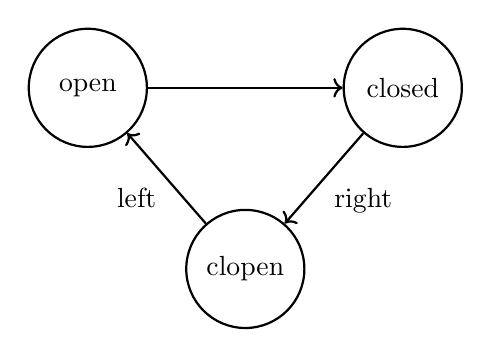
\begin{tikzpicture}[term/.style={circle,draw,minimum size={1.5cm},inner sep=5pt},auto]
    \node [thick] (o) at (0, 0) [term] {open};
    \node [thick] (c) at (4, 0) [term] {closed};
    \node [thick] (cl) at (2,-2.3) [term] {clopen};
    \draw [->,thick] (o) to node {} (c);
    \draw [->,thick] (c) to node {right} (cl);
    \draw [->,thick] (cl) to node {left} (o);
  \end{tikzpicture}
\end{center}
In the first and third disjunct $\nthTrueCapO$ denotes a mathematical sequence
of booleans of length \Cap with \False{} at every index except for index $o
\Rem \Cap$ which contains \True.

\subsubsection{The \textit{issued} token}

The $\issued(\gamma, t)$ token represents the information that the ticket $t$
has been issued. The key property of this token is that if the resource
$\issuedA$ is owned then it is possible to conclude that the lock is open.
\begin{lemma} \label{prop:issuedopen}
  Owning $\issuedA$ is sufficient to conclude that the lock is open.
  \[
\issuedA \ast \text{state}(\gamma, \kappa, \Cap, o, R, xs) \wand
        (\ownGhost{\gamma}{\circ (o, \emptyset)} \ast R \ast \bothK \ast xs = \nthTrueCapO)
  \]
\end{lemma}
This follows since $\issuedA$ is incompatible with itself per
Lemma~\ref{prop:issuedcontra} which leads to a contradiction in the
\textit{clopen} and \textit{closed} branch of the \textit{state} disjunction.

\subsubsection{The \textit{locked} predicate}

The $\lockedGKO$ predicate represents the knowledge that the lock is currently locked
along with the knowledge of what $o$ actually is. The ghost state \rightK is
included such that it is possible to conclude that the lock is in the
\textit{locked} state. This holds since the \textit{open} state contains
$\bothK$ and the \textit{clopen} state contains \rightK, both of which
contradicts with $\rightK$ per Lemma~\ref{prop:bothnocombine}.
\begin{lemma}
  From $\lockedGKO$ it is possible to conclude that the lock is closed.
  \[
    \lockedGKO \ast \text{state}(\gamma, \kappa, \Cap, o, R, xs) \wand \issuedA \ast \leftK \ast xs = \nthTrueCapO
  \]
\end{lemma}

\subsection{Proofs}
\label{sec:proofs}
We now prove the specification for each of the functions.

\subsubsection{Proof of newLock}

We sketch the proof of \textit{newLock} only at a high level as it is fairly
trivial. After executing the $\allocN$ and writing \True{} at the first index
with $(\Array \plusl 0) \gets \True$ we know that the returned value represents
an array with \True{} at index zero and \False{} at all other indices. We can
then establish the \textit{isLock} predicate by supplying a matching sequence of
booleans as a witness. For $n$ we supply the witness $0$. We must then allocate
an invariant and the ghost state it requires. Both of these can be done with the
appropriate allocation rules and by framing. When establishing the
\textit{state} disjunction in the invariant, we show the disjunct corresponding
to the lock being open.

\subsubsection{Proof of acquire}

For the \textit{acquire} function we must prove the following specification:
\[
\hoare{ \isLockA \ast \invitation(\iota, 1, \Cap) }
      { \acquire\ l }
      { o.\ \lockedGKO \ast R }
\]
Recall that the function is defined by the following \proglang code.
\begin{align*}
\langkw{let} \acquire\ l =\ &\Let \Next = \Proj2\ l in \\
    & \Let \ticket = \FAA\ \Next\ 1 in \\
    & \wait l\ \ticket; \\
    & \ticket
\end{align*}
From the \textit{isLock} predicate we know that $l$ is a triple and that there exists a location $n$ which is the second element of the triple.
Using these facts and structural rules we can step through the projection and the first \textsf{let}-expression.
We now apply the bind rule on the expression $\FAA\ n\ 1$. Since $\FAA$ is an
atomic expression we can open the lock invariant. From opening the lock
invariant we know that there exists natural numbers $o$ and $i$ such that $n$
points to $o + i$. With this points-to predicate, we can apply the
\textsc{Ht-faa} rule after which we know
\[
  n \gmapsto o + i + 1
\]
and that the $\FAA\ n\ 1$ expression evaluates to the value $o + i$.

We must now close the invariant, which per the definition means that we have to
show:
\begin{align*}
\Exists o, i, xs.
    & n \gmapsto (o + i) \ \ast a \gmapsto_{*} xs \ast \length\ \xs = \Cap\ \ast
    \invitation(\iota, i, \Cap) \ast \\
    & \ownGhost{\gamma}{\authfull ( o, \seq(o, i))} \ast
     \text{state}(\gamma, \kappa, \Cap, o, R, xs)
\end{align*}
The only part of the invariant we no longer have is $n \gmapsto o + i$. Instead,
we now have $n \gmapsto o + i + 1$. Thus, when we close the invariant we have to
provide either $o + 1$ as a witness for $o$ or $i + 1$ as a witness for $i$.
Since $o$ represents the index of who may currently access the lock and $i$
represents how many threads are waiting, it only makes sense to increment $i$.
Hence, we provide $o$ as a witness for $o$ and $i + 1$ as a witness for $i$. For
\xs we provide the same value we got when opening the invariant. Since we only
changed $i$ we can frame away the part of the invariant that does not depend on
$i$. The points-to assertion $n \gmapsto o + i + 1$ can also be framed away
since we picked $i$ exactly such that it matched the points-to assertion we had
after the fetch-and-add.

In order to close the invariant we are now left with showing
\[
  \invitation(\iota, i + 1, \Cap) \ast \ownGhost{\gamma}{\authfull(o, \seq(o, i + 1)}.
\]
From opening the invariant we have $\invitation(\iota, i, \Cap)$ and from the
precondition in the specification we have $\invitation(\iota, 1, \Cap)$. We can
combine these two facts to get $\invitation(\iota, i + 1, \Cap)$ and frame the
same thing away in the postcondition.

To show the second item we must update the authoritative ghost state we got when
opening the invariant, namely $\authfull(o, \seq(o, i))$. We can update it to
$\authfull(o, \seq(o, i) \cup \{ o + i \}) \mtimes \circ(\munit, \{ o + i \})$.
The first part of the product is exactly what we need to close the invariant,
and the second is $\issued(\munit, o + i)$ which we will need later when calling
\textit{wait}.

After closing the invariant we can evaluate the let-expression and are then left with
\begin{align*}
  & \wait l\ (o + i); o + i
\end{align*}
Since the code is a sequencing of two expressions we apply the sequencing rule.
We have the \textit{isLock} predicate, $\issued(\munit, o + i)$, and the code
$\wait l\ (o + i)$. This is fits the $\wait$ specification, which we apply. The
postcondition for the specification gives us the resource $R$ and
$\locked(\gamma, \kappa, o + i)$. Additionally, the last expression evaluates to
$o + i$. This matches precisely with the postcondition for the specification,
and we are done by framing.

\subsubsection{Proof of wait}

We now prove the specification for the \textit{wait} function.
\[
\hoare{ \isLockA \ast \issued(\gamma, t) }
      { \wait l\ t}
      { \_.\ \locked(\gamma, \kappa, t) \ast R }.
\]
Recall that the implementation of \textit{wait} is.
\begin{align*}
\langkw{let} \wait l\ t =\ &
      \Let \Array = \Proj1\ l\ in \\
    & \Let i = t \Rem (\Proj{3}\ l) in \\
    & \If \deref (\Array \plusl i) then () \Else (\wait l\ t)
\end{align*}

The definition is recursive, so we apply the \ruleref{Ht-Rec} rule, and assume
that the specification holds for any recursive call.

From the \textit{isLock} predicate we know that $l$ is a triple and that there
exists a value $a$, which is the first element of the triple, and a natural
number $\Cap$, which is the third element of the triple. With this information we
can step through the projections and the \textsf{let}-expressions. We then focus on
the condition 
\begin{equation*}
     \deref (\Array \plusl i)
\end{equation*}
with the bind rule.
We now open the invariant which contains the information that there exists an
$\xs$ such that $\Array \gmapsto_{*} \xs$. In order for the expression to make
sense, the index must be smaller than the length of the array. Fortunately, we
know from the invariant that the length of the array is $\Cap$ and $t \Rem \Cap$
is certain to be smaller than $\Cap$. From this we can show that the load
expression evaluates to a boolean $b$ where
\begin{equation} \label{eq:bvalue}
 b = \xs_{(t \Rem \Cap)}
\end{equation}
Since $b$ is a boolean it is either true or false, and we proceed by case
analysis on $b$.

We first consider the case where $b = \false$ as it is the simplest case.
It suffices to show:
\begin{align*}
     & \If \False then () \Else (\wait l\ t)
\end{align*}
We cannot step forward through the code until after we close the invariant. We
still have everything from opening the invariant, so we simply use the exact same
values as witnesses to close the invariant. We then apply \ruleref{Ht-If-False}
which leaves us with the code
\begin{align*}
   \wait l\ t
\end{align*}
This is a recursive call of \textit{wait} and we can now apply the
specification we assumed when we used the \ruleref{Ht-Rec} rule earlier. This
concludes the first case.

In the second case we have $b = \true$. Intuitively, we are in this case because
the lock is open. Not only is the lock open, our ticket $t$ should be equal to
the ticket which now grants access to the lock, namely $o$. If we can show this,
then we have $\issuedA$, and we can then use Lemma~\ref{prop:issuedopen} to
conclude that the lock is open.

Consider the $\text{state}(\gamma, \kappa, \Cap, o, R, xs)$ part of the
invariant:
\begin{align*}
        & (\ownGhost{\gamma}{\circ (o, \emptyset)} \ast R \ast \bothK \ast xs = \nthTrueCapO) \lor \\
        & (\issuedA \ast \rightK \ast xs = \replicate(\false, \Cap)) \lor \\
        & (\issuedA \ast \leftK \ast xs = \nthTrueCapO).
\end{align*}

The second case of the disjunction contains the equality
\begin{align*}
  \xs = \replicate(\false, \Cap)
\end{align*}
This states that $\xs$ is a list containing only \false. This is a
contradiction, as we have just read $\true$ at an index in the array. In
particular, we know that $b = \true$ and $b = \xs_{(t \Rem \Cap)}$. It is easy
to show that $\xs = \replicate(\false, \Cap)$ implies that $\xs_i = \false$ for
any $i$ smaller than $\Cap$. And, since $t \Rem \Cap$ is certainly smaller than
$\Cap$ we have the desired contradiction.

Both of the remaining cases contains the equality $\xs = \nthTrueCapO$.
Combining this with Equation \ref{eq:bvalue} we get
\[
  \nthTrueCapO_{(t \Rem \Cap)} = \true.
\]
Recall that $\nthTrueCapO$ denotes a list that only contains \true{} at index $o \Rem \Cap$.
Thus the above implies
\begin{equation} \label{eq:otremeq}
  o \equiv t \quad (\text{mod } \Cap).
\end{equation}
This is, unfortunately, not enough to prove $t = o$. It could, for instance,
still be the case that $t = o - \Cap$ or $t = o + \Cap$. However, considering
how the ABQL works neither of these can actually happen.
\begin{itemize}
  \item We can never have a ticket that is smaller than $o$. Then it would
    already have been our turn to acquire the lock.
  \item Our ticket can not be larger than $o + \Cap$. Intuitively, $t - o$
    represents how many threads are currently in front of us in the queue to
    acquire the lock. But, because at most $\Cap$ threads can ever wait for the
    lock, our position in the queue can be no larger than $\Cap$.
\end{itemize}
Fortunately, both of these intuitions are encoded in the definitions and can be
shown as follows.

We have $\issued(\gamma, t) = \ownGhost{\gamma}{\circ(\munit, \{ t \})}$ and
$\ownGhost{\gamma}{\authfull(o, \seq(o, i)}$. By using
Lemma~\ref{prop:ticketbound} we have
\[
  o \leq t < o + i
\]
This shows the first item above, that $t$ can not be smaller than $o$.

From opening the invariant we have 
$\invitation(\iota, i, \Cap)$. We can thus use Lemma~\ref{prop:iLtCap} to
conclude that $i \leq \Cap$. Put together with the above, we have the second
item.
\[ t < o + i \leq o + \Cap. \] This is sufficient to show that $t = o$. We leave
the details as an exercise.
\begin{exercise}
  Show that given $\Cap, t, o \in \mathbb{Z}$ where $0 < \Cap$ and $o \leq t < o
  + \Cap$ the equality $t \Rem \Cap = o \Rem \Cap$ implies that $ t = o $.
\end{exercise}


This means that in both of the remaining cases we have $\issued(\gamma, o)$ and
per Lemma~\ref{prop:issuedcontra} we now know that the lock must be in the
state corresponding to open.

In other words, from opening the lock invariant we now also have $\bothK$, the resource $R$, and the partial information $\ownGhost{\gamma}{\circ(o, \emptyset)}$.
We can split $\bothK$ into a $\leftK$ and a $\rightK$.
This means that we have $\issued(\gamma, o)$, $\leftK$, and, from opening the invariant, $xs = \nthTrueCapO$.
These are exactly the things needed to show the \textit{closed} state of the disjunction in the invariant.
Thus we can close the invariant providing the same variables we initially got for $o$, $i$, and $\xs$ followed by framing.

We have now closed the invariant and can step further into the code. We use the
\ruleref{Ht-If-True} rule and are left with
\[
  ()
\]
Hence, the only thing left to show is the postcondition. This includes $R$ and
$\lockedGKO = \ownGhost{\gamma}{\circ(o, \emptyset)} \ast \rightK$. Both of
these follow from framing as we have these from the invariant.

\subsubsection{Proof of release}

In this section we describe the proof of the specification for the
\textit{release} function. Recall the specification:
\[
\hoare{ \isLock(\gamma, \iota, \kappa, l, \Cap, R) \ast \locked(\gamma, \kappa, o) \ast R }
      { \release\ l\ o }
      { \_.\ \invitation(\iota, 1, \Cap) }
\]
Also recall that \textit{release} is defined as follows.
\begin{align*}
  \langkw{let} \release\ l\ o =\ & \Let \Array = \Proj1\ l in \\
                                 & \Let \Cap = \Proj{3}\ l in \\
                                 & \Array \plusl (o\ `rem`\ \Cap) \gets \False ; \\
                                 & \Array \plusl (o + 1\ `rem`\ \Cap) \gets \True
\end{align*}
We can evaluate the two let expressions using the facts from the isLock
predicate which leaves us with
\begin{align*}
  & \Array \plusl (o\ `rem`\ \Cap) \gets \False ; \\
  & \Array \plusl (o + 1\ `rem`\ \Cap) \gets \True
\end{align*}

Before we proceed any further, let us take a step back and consider how the proof
must proceed. In the code above, there are two store operations that write into
the array. Since the points-to predicate for the array is inside the invariant
we must open the invariant twice. Each time we open the invariant we must
consider the state$(\gamma, \kappa, \Cap, o, R, \xs)$ disjunction inside the
invariant.

Since the lock is closed when we open the invariant for the first time, we
should be able to conclude that it is in the \textit{closed} state. We then set
the single \True{} value in the array to \False. Hence, we must close the
invariant in the \textit{clopen} state. When we open the invariant for the
second time, we should be able to conclude that the disjunction is still in the
\textit{clopen} state. Finally, after the last store operation we should be able
to close the invariant in the \textit{open} state.

We use the bind rule to focus on the first store operation.
\begin{align*}
  \Array \plusl (o\ `rem`\ \Cap) \gets \False
\end{align*}
We now open the invariant and get the existence of $o'$, $i$, and \xs such that
\begin{align*}
  & n \gmapsto (o' + i) \ast
    \Array \gmapsto_{*} \xs \ast \length\ \xs = \Cap \ast \\
  & \invitation(\iota, i, \Cap) \ast
    \ownGhost{\gamma}{\authfull ( o', \seq(o', i))} \ast
    \text{state}(\gamma, \kappa, \Cap, o', R, xs)
\end{align*}
Since we have $\rightK$ we can conclude that the $\text{state}(\gamma, \kappa,
\Cap, o', R, xs)$ disjunction is in the last state as the first branch contains
$\bothK$ and the second branch contains $\rightK$---both of which lead to a
contradiction when combined with $\rightK$. We therefore additionally know.
\[
  \text{issued}(\gamma, o') \ast \leftK \ast \xs = \nthTrue(\Cap, o' \Rem \Cap).
\]
When closing the invariant we want to show the middle part of the state
disjunction, and hence our goal is to show
\[
  \text{issued}(\gamma, o') \ast \rightK \ast \xs = \replicate(\false, \Cap).
\]
The only thing we must work for is $\xs = \replicate(\false, \Cap)$ as the
other properties can be framed away. Fortunately, this is exactly what we
expect to be able to show after stepping through the store as this operation is
supposed to overwrite the single \True{} in the array with a \False. But, notice
that we are setting the array using the value $o$, but, that the information
from the invariant describes where the \True{} value is in the list in terms of
$o'$. We therefore want to show that $o$ and $o'$ are in fact equal. To do
this we combine $\ownGhost{\gamma}{\circ(o, \emptyset)}$ from the
$\locked(\gamma, \kappa, o)$ predicate in the precondition with 
$\ownGhost{\gamma}{\authfull ( o', \seq(o', i))}$ from the invariant.

We now have $ \xs = \nthTrue(\Cap, o' \Rem \Cap)$ and the code
\begin{align*}
  \Array \plusl (o\ `rem`\ \Cap) \gets \False
\end{align*}
From this we can show the postcondition $\xs = \replicate(\false, \Cap)$.
This is what we need to close the invariant in the \textit{clopen} state.
We frame everything else away.

We now focus on the next store operation. We still have the resources we started
with except that instead of \rightK we now have \leftK, and the code is
\begin{align*}
  \Array \plusl (o + 1\ `rem`\ \Cap) \gets \True
\end{align*}
We again open the invariant. Similarly to how we previously used \rightK to
determine the state of the disjunction in the lock we now use \leftK to
determine that the lock is still in the clopen state. We therefore have $\xs =
\replicate(\false, \Cap)$ and $\Array \gmapsto \replicate(\false, \Cap)$. After
executing the store operation we thus have
\[
  \Array \gmapsto \nthTrue(\Cap, (o + 1) \Rem \Cap)
\]
We are now ready to close the invariant for the last time.
When closing the invariant in the open state we must provide three witnesses and show the following.
\begin{align*}
  \Exists o, i, xs. & n \gmapsto (o + i) \ \ast a \gmapsto_{*} xs \ast \length\ \xs = \Cap\ \ast \\
    & \invitation(\iota, (i - 1), \Cap) \ast \ownGhost{\gamma}{\authfull ( o, \seq(o, i))} \ast \\
    &  \ownGhost{\gamma}{\circ (o, \emptyset)} \ast R \ast \bothK \ast xs = \nthTrueCapO
\end{align*}
For $o$ we provide $o + 1$, since we have now effectively moved the \true{}
value in the array one element to the left. For $\xs$ we provide
$\nthTrue(\Cap, (o + 1) \Rem \Cap)$. When we opened the invariant every entry in
\xs{} was \false{} but we have updated one entry to \true. For $i$ we provide
$i - 1$. We do this because invariant contains $n \gmapsto o + i$ and since we
are providing $o + 1$ in the place of $o$ we have to establish
$n \gmapsto (o + 1) + i$. But, we have not changed what $n$ points to so we
still only have $n \gmapsto o + i$. The only way we can make this work is to use
$i - 1$ as the witness for $i$.

With this choice of witnesses we can immediately frame away $R$ and the
points-to predicate for the array. The equality involving the length is
trivially true. We show \bothK{} by combining the \leftK{} and the \rightK{}
that we have with \ruleref{Own-op} followed by framing.

For the points-to predicate we have $n \gmapsto o + i$ and are to show
$n \gmapsto o + 1 + (i - 1)$. Since we are working with natural numbers
$(o + 1) + (i - 1)$ is only equal to $o + i$ if $i$ is greater than 0. We thus
have the points-to predicate if we can show that $i$ is greater than 0.

From opening the invariant we have both
$\issuedA = \ownGhost{\gamma}{\circ(\munit, \{o\})}$ and
$\ownGhost{\gamma}{\authfull ( o, \seq(o, i))}$. We can combine these using
\ruleref{Own-op} and then conclude that
\[ \circ(\munit, \{o\}) \mtimes \authfull(o, \seq(o,i)) \] is valid from the
\ruleref{Own-valid} rule. From the definition of valid in the authoritative
resource algebra, this implies that $o \in \seq(o, i)$. If $i$ was 0 then
$\seq(o, i)$ would be the empty set so this can not be the case. With this fact
we can rewrite the goal $n \gmapsto ((o + 1) + (i - 1))$ into $n \gmapsto o + i$
which we can then frame away.

Notice that since we decremented the value of $i$ when we closed the invariant
we only have to show $\invitation(\iota, i - 1, \Cap)$. On the other hand, the
postcondition of \textit{release} requires us to show
$\invitation(\iota, 1, \Cap)$. This adds up nicely. By using \ruleref{Own-op} we
split the $i$ invitations we have into one ghost state with 1 invitation and one
ghost state with $i - 1$ invitations. We can then frame both the aforementioned
goals away.

The only thing that remains to show is:
\begin{align*}
  \ownGhost{\gamma}{\authfull ( o + 1, \seq(o + 1, i - 1))} \ast \ownGhost{\gamma}{\circ (o + 1, \emptyset)}
\end{align*}
To do that we have $\ownGhost{\gamma}{\circ(\munit, \{o\})}$ and $\ownGhost{\gamma}{\authfull ( o, \seq(o, i))}$ from opening the invariant and $\ownGhost{\gamma}{\circ(o, \emptyset)}$ from the $\lockedGKO$ predicate in the original precondition.
It is clear that we must make a frame preserving update in order to achieve this.
Specifically we need the frame preserving update
\[
    \circ (o, \emptyset) \mtimes \circ (\munit, \{ o \}) \mtimes \authfull (o, \seq(o, i) \})
    \mupd
    \circ (o + 1, \emptyset) \mtimes \authfull (o + 1, \seq(o + 1, i - 1 ))
    .
\]
\begin{exercise}
  Show the above frame preserving update.
\end{exercise}


Using the \ruleref{Ghost-update} rule on this frame preserving update
we are done with the proof of \textit{release}.

\subsection{Discussion}

We have now completed the proof of the specification for the ABQL, a lock that can be used
by at most a fixed number of participating threads.
In particular, we have seen how the specification of the ticket lock can be
extended to express the restrictions using the concept of invitations and we have
verified that the implementation meets the specification using a suitable resource
algebra for invitations.

%%% Local Variables:
%%% mode: latex
%%% TeX-master: "../main.tex"
%%% End:



\section{Modular Specifications for Concurrent Modules}
\label{sec:modular-specs-of-concurrent-modules}

In the previous sections we have seen several examples and case studies involving specifications of concurrent modules.
In particular, in Section~\ref{sec:authoritative-ra} we presented several different specifications of a simple counter module.
In general, it is difficult to find out what is the ``right'' specification to give to a (concurrent) module.
Often we would like to have a specification which is sufficiently general that it can be used by many, ideally \emph{all possible}, different clients.
In this section we give some ``methodological advice'' on how to give modular specifications for concurrent modules that are sufficiently general that they can be instantiated by many diverse clients.
In particular, we present a new specification of the concurrent counter module, which is \emph{more modular}, in the sense that the earlier given specifications can be derived from it (\emph{without reference to the code of the counter, only using the abstract predicates}).
Moreover, we also show how this modular specification of the counter module allows us to give a modular proof of the ticket lock, \ie\ a proof of the ticket lock which only depends on the \emph{specification} of the counter module, \emph{not} on the concrete implementation.
We include this section for the obvious reason that modularity is a key point we have been striving for all along, but also because it gives us an additional opportunity to show how Iris's higher-order logic supports quite advanced modular specifications.

The methodology we present is a \emph{higher-order approach to modular specifications of concurrent modules}.
It stems from~\cite{hocap-conf}, which was based on~\cite{Jacobs:Piessens:2011}.
It is closely related to the notion of logical atomicity from the TaDa logic~\cite{TaDa}.
The examples, the concurrent counter module and the ticket lock, are from~\cite{DINSDALEYOUNG20181}, which contains a presentation and discussion of these examples using TaDa-style logical atomicity.
This section is supposed to be an introduction to the topic of modular specifications for concurrent modules, please see the mentioned references for further discussion.


We now outline the overall idea of the methodology; it is perhaps a little tricky to understand at first, so it may be easiest to read this description quickly at first, and then study the examples below and return to the description again.

We consider concurrent modules which have some state and some methods operating on the state.
A concrete example could be a concurrent stack module.
To specify a concurrent module, we decide on what the mathematical model of the abstract state should be, and in particular how the model allows for sharing.
For the concurrent stack module, a natural choice is to model the abstract state of the stack by a mathematical sequence of natural numbers (assuming that the elements of the stack are simply natural numbers). 
We will use a ghost variable to keep track of the contents of the abstract state of the module, so for the concurrent stack we will have a ghost resource whose contents will be a mathematical sequence of numbers.
Now consider the specification of a method. Typically, it will involve a modification of the abstract state of the module.
For example, for the concurrent stack, a push method is supposed to change the abstract state of the module, by inserting the element being pushed into the front of the mathematical sequence modeling the abstract state of the stack.

Since we are in a concurrent setting, it matters \emph{when} the state of the module changes, and when the abstract state changes, a client will typically also have to update some invariants and protocols of its own.
However, the module, of course, cannot know how different clients wish to update their invariants when the abstract state of the module changes.
Therefore we \emph{parameterize} the method specification by a view shift, which (1) describes how the abstract state is supposed to change and (2) describes how other invariants should be updated. 
The idea is that, when we prove the specification of the method of the module, then we can use this view shift to update the abstract state
of the module; typically, we will then also show that the concrete state of the module matches the new abstract state of the module.
Thus it is the \emph{client} of the module who has to prove that the abstract state of the module can be changed as described by the view shift,
since the client has to provide a proof of the view shift. (Perhaps it is surprising that the \emph{client} can prove that the abstract state of
the module can be changed, but notice that the client only considers the \emph{abstract state} of the module, which is tracked using ghost state ---
the modifications to the actual \emph{concrete state} of the module are proved to match the abstract state change when we prove the module method specification.)
Since the module cannot know which other invariants the client has, we also parameterize the specification by predicates intended to describe those. 


\newcommand{\wkincrC}{\operatorname{wk{\_}incr}}
\newcommand{\Cnt}{\operatorname{Cnt}}

\subsection{Modular Specification of Concurrent Counter Module}
\label{sec:modular-conter}

\paragraph{Counter Implementation}

The counter implementation we will consider is the same as in Section~\ref{sec:authoritative-ra}, except we add an additional \emph{weak increment} ($\wkincrC$) method.
Its definition is the following
\begin{align*}
  \wkincrC \ell = \ell \gets  1 + \deref \ell.
\end{align*}
The intention is that clients should only call the weak increment method when the client knows that it is safe to do so, \ie\ when the client knows that only one thread will increment the counter.
Since the increment is not atomic 

\renewcommand{\Cnt}{\operatorname{Cnt}}
\newcommand{\abstractstatefrac}[3]{#1 \Mapsto\kern-0.5ex\tfrac{1}{#2} #3}
\newcommand{\abstractstate}[3]{#1 \Mapsto^{#2}_{\circ} #3}
\newcommand{\abstractstatefullfrag}[2]{#1 \Mapsto_{\circ} #2}
\newcommand{\abstractstateauth}[2]{#1 \Mapsto_{\bullet} #2}
\newcommand{\CntInvName}{c}
\newcommand{\CntInv}{\operatorname{CntInv}}

\paragraph{A Resource Algebra for the Abstract State of the Counter}

We model the abstract state of the counter by a natural number.
We will use a resource algebra for keeping track of the abstract state of the counter module.
The resource algebra is the authoritative resource algebra (from Example~\ref{example:authoritative-RA}) over the product of the resource algebra of fractions (from Example~\ref{example:resource-algebra-of-fractions}) and the agreement resource algebra (from Example~\ref{example:agreement-resource-algebra}) on the set of natural numbers $\nat$ (the type of the model of the abstract state of the counter).
The product of the two last resource algebra is not a unital resource algebra.
In order to apply the authoritative resource algebra construction we wrap the product in the option resource algebra (from Example~\ref{example:option-resource-algebra}).
The resulting construction is $\authm((\QQ_{01} \times \nat)_?)$.

We write $\abstractstate{\gamma}{q}{m}$ for the ghost ownership assertion $\ownGhost{\gamma}{\authfrag (q,m)}$ of the fragmental element $\authfrag (q, m)$ to reflect the intuitive reading of this ghost ownership assertion as ``there is a ghost heap, which maps $\gamma$ to $m$ with fraction $q$''.
In particular, we write $\abstractstatefrac{\gamma}{k}{m}$ when the fraction $q$ is $\frac{1}{k}$.
In case when $q = 1$ we write $\abstractstatefullfrag{\gamma}{m}$.
We write $\abstractstateauth{\gamma}{m}$ for the ownership assertion $\ownGhost{\gamma}{\authfull (1, m)}$ of the authoritative element $\authfull (1, m)$.
It is a simple exercise to verify that for all $n, m$ and $p, q$ we have the following entailments.
\begin{align}
  \abstractstate{\gamma}{q}{m} \ast \abstractstate{\gamma}{q}{n} \proves n = m \label{eq:ra-abstract-state-eq}\\
  \abstractstate{\gamma}{p}{m} \ast \abstractstateauth{\gamma}{n} \proves n = m \label{eq:ra-abstract-state-auth-eq}\\
  \abstractstate{\gamma}{p}{m} \ast \abstractstate{\gamma}{q}{m} \provesIff \abstractstate{\gamma}{p+q}{m} \label{eq:ra-abstract-state-sum}  \\
  \abstractstate{\gamma}{1}{m} \ast \abstractstateauth{\gamma}{m} \proves \pvs \abstractstate{\gamma}{1}{n} \ast \abstractstateauth{\gamma}{n} \label{eq:ra-abstract-state-upd}
\end{align}
The first property means that everybody in possession of the partial knowledge (fraction $q$ less than $1$) agrees on the value of the counter, the second property states that anyone in possession of the partial knowledge agrees with the authoritative part on the value of the counter, 
 the third property states how the abstract predicate can be split, and the last property states that anybody in full possession of the fragmental state of the counter and the authoritative state of the counter can update both.
\begin{exercise}
  \label{ex:counter-ghost-state-1}
  Prove the preceding properties of the assertions $\abstractstate{\gamma}{q}{m}$ and $\abstractstateauth{\gamma}{m}$.
\end{exercise}


\paragraph{Modular Counter Specification}

In the following we assume $\mask$ is an infinite set of invariant names.

The modular counter specification is as follows, we explain it below.
In the specification for $\wkincrC$, $P$ and $Q$ range over $\Prop$, $v$ over $\Val$, $q$ over fractions $\QQ_{01}$, and $m$ over $\nat$.
\begin{align*}
  & \Exists \Cnt : \Val \to \textlog{GhostName} \to \textlog{InvName} \to \Prop.\\
  & \qquad \persistently\left(\All v, \gamma, c. \Cnt(v,\gamma,c) \implies \persistently \Cnt(v,\gamma,c)\right) \\
  & \land \quad\hoare{\TRUE}{\newC()}{v.\Exists \gamma, c.  \Cnt(v,\gamma,c) \ast \abstractstate{\gamma}{1}{0}}[\mask] \\
  & \land \quad\All \gamma, c, P, Q, v.
    \begin{array}[t]{l}
    \left(\All m. (\abstractstateauth{\gamma}{m} \ast P) \vs[\mask\setminus{\{\CntInvName\}}]
    (\abstractstateauth{\gamma}{m} \ast Q(m))\right) \implies \\
      \hoare{\Cnt(v,\gamma, c) \ast P}{\readC(v)}{u. \Cnt(v,\gamma, c) \ast Q(u)}[\mask]
    \end{array}\\
  & \land \quad\All \gamma, c, P, Q, v.
    \begin{array}[t]{l}
    \left(\All m. (\abstractstateauth{\gamma}{m} \ast P) \vs[\mask\setminus{\{\CntInvName\}}]
    \left(\abstractstateauth{\gamma}{(m+1)} \ast Q(m)\right)\right) \implies \\
      \hoare{\Cnt(v,\gamma,c) \ast P}{\incrC(v)}{u. \Cnt(v,\gamma,c) \ast Q(u)}[\mask]
    \end{array}\\
  & \land \quad \All \gamma, c, P, Q, v, q, m.
    \begin{array}[t]{l}
    \left(\abstractstateauth{\gamma}{m} \ast \abstractstate{\gamma}{q}{m} \ast P \vs[\mask\setminus{\{\CntInvName\}}]
     \abstractstateauth{\gamma}{(m+1)}  \ast Q\right) \implies \\
      \hoare{\Cnt(v,\gamma,c) \ast \abstractstate{\gamma}{q}{m}\ast P}{\wkincrC(v)}{u. u=\TT \ast \Cnt(v,\gamma,c) \ast Q}[\mask]
    \end{array}
\end{align*}

The idea is that the abstract predicate $\Cnt(v,\gamma,c)$ expresses that $v$ represents a counter, whose abstract state is kept in the ghost variable $\gamma$,
and which uses invariant name $c$.
As usual, $\Cnt(v,\gamma,c)$ is persistent so that we can share it among several threads.

The postcondition of $\newC$ says that a counter is created and, moreover, that the abstract state of the counter is $0$. The client of the counter gets  ownership of the fragmental part ($\abstractstate{\gamma}{1}{0}$) of the abstract state, which means that if the client gets access to the authoritative part ($\abstractstateauth{\gamma}{0}$), which is kept by the counter module, then it can update the abstract state of the counter.
The fragmental and authoritative parts together represent the abstract state of the counter from different angles.
The authoritative part $\abstractstateauth{\gamma}{0}$ provides the \emph{module view} of the abstract state, and the fragmental part $\abstractstate{\gamma}{1}{0}$ provides the \emph{client view} of the abstract state.
Those two views have to be synchronized.
This means that the counter module cannot update the abstract state of the counter ``on its own'', just from the module view (remember that the idea of the methodology is that the module cannot know what should happen when the abstract state changes and hence it delegates updating of the abstract state to the client of the module).

Now consider the specification of $\incrC$. To use this specification, the client must show the view shift
\begin{align*}
\All m. (\abstractstateauth{\gamma}{m} \ast P) \vs[\mask\setminus{\{\CntInvName\}}] (\abstractstateauth{\gamma}{(m+1)} \ast Q(m)),
\end{align*}
and then it gets the Hoare triple  $\hoare{\Cnt(v,\gamma,c) \ast P}{\incrC(v)}{u. \Cnt(v,\gamma,c) \ast Q(u)}[\mask]$.
The view shift expresses that the $\incrC$ will increment the abstract state of the counter; 
the predicates $P$ and $Q$ are universally quantified and can thus be instantiated by the client to coordinate updates to invariants held by the client.
The Hoare triple expresses that one may call $\incrC$ if one has a $\Cnt(v,\gamma,c)$ resource.

The specification of $\readC$ is similar to the specification of $\incrC$, except that the abstract state does not change.
Even though the abstract state does not change, we still parameterize the specification by a view shift, because that will allow a client to
update its own invariants appropriately when it learns about the abstract state of the counter (by instantiating $P$ and $Q$ as necessary).
We will show examples of how this can be done below.

Note that the quantification over the abstract state $m$ of the counter in the view shifts for $\incrC$ and $\readC$ captures the point that a client cannot know (if the counter is shared by different threads) what the abstract state is --- because other threads may call methods on the counter concurrently.

In the specification of $\wkincrC$, the value of the counter $m$ is quantified over both the view shift and the Hoare triple.
Moreover, to call $\wkincrC$, the client must have fragmental ownership of the abstract state of the counter (note the $\abstractstate{\gamma}{q}{m}$ in the precondition of the Hoare triple); this captures the idea that no other thread can have full ownership of the abstract state and hence cannot update the abstract state ``under our feet'', which is in accordance with the idea that a client should only call $\wkincrC$ when it knows that no other thread can modify the counter.
In the specifications for $\incrC$ and $\readC$, the predicate $Q$ is parameterized by the abstract state of the counter (because we do not know up front what
the abstract state is), but in the specification for $\wkincrC$, the predicate $Q$ need not be parameterized by the abstract state of the counter, since
the client already keeps track of it ($\abstractstate{\gamma}{q}{m}$). 

Finally, we comment on the mask annotation on the view shifts: since the mask is $\mask\setminus{\{\CntInvName\}}$, the client may use (open and close) all the invariants in $\mask$ when showing the view shift, except the invariant named $c$ used by the counter module.
That is also the reason why we parameterize $\Cnt$ by $c$ (rather than hiding $c$ behind an existential, as we have done in earlier examples).
(In Coq, we use invariant name spaces to keep tract of these invariant names, see Section~\ref{sec:invariant-namespaces}.)

\paragraph{Showing that the Implementation meets the Modular Counter Specification}
We now outline the proof that the counter implementation meets the above modular specification.
We naturally use an invariant to share the state of the counter. The invariant connects the concrete value of the counter to the abstract state of the counter, which in this case is simply the same value as the concrete value stored in the reference of the counter module.
\footnote{Generally, in this methodology, the abstract state is an appropriate mathematical abstraction of the contents of the module, \eg\ the abstract state for a concurrent stack module could be a mathematical sequence of values.}
%
\begin{align*}
  \CntInv(v,\gamma) & = \Exists m. v\pointsto m \ast \abstractstateauth{\gamma}{m}\\
  \Cnt(v,\gamma,c) & = \knowInv{\CntInvName}{\CntInv(v,\gamma)}
\end{align*}
%
With this definition of the abstract $\Cnt$ predicate, it is not hard to show that the different methods
meet the specifications. Here we just outline the proof for the $\incrC$ method, and leave the other (easier) ones as
an exercise.

For $\incrC$ we first assume the given view shift, and the proceed to show the Hoare triple.
To that end, since $\incrC$ is a recursive function we proceed, as usual, by L{\"o}b induction. To dereference the reference we open the invariant and then close it again. Then we get to the $\CAS$ instruction.
We open the invariant and thus get ownership of the authoritative part of the abstract state, \ie{} we get
$\abstractstateauth{\gamma}{m}$ for some $m$.
The interesting case is when it succeeds (otherwise we just end up recursing so the proof succeeds by applying the L{\"o}b induction hypothesis).
In this case we get that the reference now points to $m+1$ (since the $\CAS$ succeeded). 
Now we want to apply the view shift, so we instantiate it with $m$, and then we can apply it.
This we can do since we both have $\abstractstateauth{\gamma}{m}$ and $P$ (we have $P$ from the precondition in the Hoare triple).
By the view shift we have $\abstractstateauth{\gamma}{(m+1)}$ and $Q(m)$.
Thus, since we now both have that the reference points to $m+1$ and we also have $\abstractstateauth{\gamma}{(m+1)}$,
we can close the counter invariant, and thus we obtain the required postcondition.
So, in summary, the key point to notice is that the abstract state of the counter is updated by an application
of the view shift which the specification is parameterized by.

\begin{exercise}
  Show the specifications for $\newC$, $\readC$, and $\wkincrC$.
\end{exercise}

\subsubsection{Deriving Counter with Contributions from the Modular Counter Specification}
\label{sec:deriving-ccounter-from-modular-conter}

In this subsection we sketch how we may use the modular counter specification from above to \emph{derive} a counter-with-contributions specification from Exercise~\ref{exercise:precise-counter-specification} in Section~\ref{sec:authoritative-ra}.

The idea is to proceed much as in Exercise~\ref{exercise:precise-counter-specification}, except that now we have to use the \emph{abstract state} of the counter (as a client of the modular counter specification that is all we can use!).
Thus we let $\isCounter$ be the predicate
\begin{align*}
    \isCounter(\ell, n, \gamma_{1}, \gamma_{2}, c, p) =
    \ownGhost{\gamma_{1}}{\authfrag (p, n)} \ast \Exists \iota\in\mask\setminus\{c\} . \knowInv{\iota}{\Exists m . \abstractstatefullfrag{\gamma_{2}}{m} \ast \ownGhost{\gamma_{1}}{\authfull (1, m)}}
    \ast \Cnt(\ell,\gamma_{2},c).
\end{align*}
where we use the same authoritative resource algebra as we did for the verification of the counter with contributions previously.
%
Note the similarity to the earlier definition in Exercise~\ref{exercise:precise-counter-specification}! In the definition of $\isCounter$, the predicate
$\Cnt(\ell,\gamma_{2},c)$ expresses that $\ell$ is a counter, whose abstract state is tracked by $\gamma_{2}$, and in the invariant we use 
$\abstractstatefullfrag{\gamma_{2}}{m}$ to record that the abstract state of the counter is $m$ (note how this ghost state plays a role similar to
the role played by $\ell\pointsto m$ in  Exercise~\ref{exercise:precise-counter-specification}).
Also note that $\isCounter(\ell, n, \gamma_{1}, \gamma_{2}, c, p)$ is persistent.

With this definition in place, we can prove the following specifications:
\begin{align*}
    &\hoare{\TRUE}{\newC \TT}{u.\Exists \gamma_{1},\gamma_{2}, c . \isCounter(u, 0, \gamma_{1}, \gamma_{2}, c, 1)}\\
    &\All p . \All \gamma_{1},\gamma_{2}. \All c . \All v . \All n . \hoare{\isCounter(v, n, \gamma_{1}, \gamma_{2}, c, p)}{\readC v}{u.u \geq n \ast \isCounter(v, n, \gamma_{1}, \gamma_{2}, c, p)}\\
    &\All \gamma_{1},\gamma_{2} . \All c . \All v . \All n . \hoare{\isCounter(v, n, \gamma_{1}, \gamma_{2}, c, 1)}{\readC v}{u.u = n \ast \isCounter(v, n, \gamma_{1}, \gamma_{2}, c, 1)}\\
    &\All p . \All \gamma_{1},\gamma_{2} . \All c. \All v . \All n . \hoare{\isCounter(v, n, \gamma_{1},\gamma_{2}, c, p)}{\incrC v}{u.u = \TT \ast \isCounter(v, n+1,\gamma_{1},\gamma_{2}, c, p)}
\end{align*}

We sketch the proof for $\incrC$, and the leave the others as an exercise.
We assume the precondition, which gives us $\Cnt(v,\gamma_{2}, c)$, as is necessary for using the modular counter specification for $\incrC$.
We instantiate $P$ and $Q$ in the modular $\incrC$ specification by $P=\ownGhost{\gamma_{1}}{\authfrag (p, n)}$ and
$Q=\lambda x.\ownGhost{\gamma_{1}}{\authfrag (p, n+1)}$. Now we need to show the view shift
\begin{align*}
  \abstractstateauth{\gamma_{2}}{m} \ast \ownGhost{\gamma_{1}}{\authfrag (p, n)}
  \vs[\mask\setminus\{c\}]
  \abstractstateauth{\gamma_{2}}{(m+1)} \ast \ownGhost{\gamma_{1}}{\authfrag (p, n+1)}.
\end{align*}
We do this by opening the invariant $\iota$, which gives us $\abstractstatefullfrag{\gamma_{2}}{k} \ast \ownGhost{\gamma_{1}}{\authfull (1, k)}$, for some $k$.
By the properties for resource algebra for abstract state \eqref{eq:ra-abstract-state-auth-eq} we conclude that $k=m$.
Using~\eqref{eq:ra-abstract-state-upd}, we can update the abstract state $\abstractstatefullfrag{\gamma_{2}}{k} \ast \abstractstateauth{\gamma_{2}}{k}$ to $\abstractstatefullfrag{\gamma_{2}}{k+1} \ast \abstractstateauth{\gamma_{2}}{k+1}$.
By the properties of the authoritative resource algebra we can also update $\ownGhost{\gamma_{1}}{\authfrag (p, n)}\ast \ownGhost{\gamma_{1}}{\authfull (1, k)}$ to $\ownGhost{\gamma_{1}}{\authfrag (p, n+1)}\ast\ownGhost{\gamma_{1}}{\authfull (1, k+1)}$.
With this we can close the $\iota$ invariant again.
Recalling that $k=m$, the resources we have left are exactly the $\abstractstatefullfrag{\gamma_{2}}{(m+1)} \ast \ownGhost{\gamma_{1}}{\authfrag (p, n+1)}$, as required for completing the proof of the view shift.

Since we have shown the view shift, we now get the Hoare triple
\begin{align*}
\hoare{\Cnt(v,\gamma_{2},c) \ast \ownGhost{\gamma_{1}}{\authfrag (p, n)}}{\incrC(v)}{u. u=\TT \ast \Cnt(v,\gamma_{2},c) \ast \ownGhost{\gamma_{1}}{\authfrag (p, n+1)}}  
\end{align*}
By the definition of $\isCounter$, we not only have $\Cnt(v,\gamma_{2},c)$, but also
$\ownGhost{\gamma_{1}}{\authfrag (p, n)}$. Hence we conclude from the Hoare triple above that we can indeed call $\incrC(v)$ and obtain 
$\Cnt(v,\gamma_{2},c) \ast \ownGhost{\gamma_{1}}{\authfrag (p, n+1)}$, which, together with the invariant $\iota$, suffices to conclude
$\isCounter(v, n+1,\gamma_{1},\gamma_{2}, c, p)$, as required.


\subsubsection{Deriving Sequential Counter from Modular Counter Specification}
\label{sec:deriving-sequential-from-modular-conter}

\newcommand{\SeqCnt}{\operatorname{SeqCnt}}

Here is a specification for a counter that can be used in a sequential context only:
\begin{align*}
  & \Exists \SeqCnt : \Val \to \textlog{GhostName} \to \textlog{InvName} \to \nat \to \Prop.\\
  & \qquad\All n. \hoare{\TRUE}{\newC()}{v.\Exists \gamma, c.  \SeqCnt(v,\gamma,c,0)}  \\
  & \land \quad\All \gamma, c, v, n.
    \begin{array}[t]{l}
      \hoare{\SeqCnt(v,\gamma, c, n)}{\readC(v)}{u. u = n \ast \SeqCnt(v,\gamma, c, n)}
    \end{array}\\
  & \land \quad\All \gamma, c, v, n.
    \begin{array}[t]{l}
      \hoare{\SeqCnt(v,\gamma,c, n)}{\incrC(v)}{u. u = n \ast \SeqCnt(v,\gamma,c,n+1)}
    \end{array}\\
\end{align*}
Since the representation predicate
$\SeqCnt(v,\gamma,c,n)$ is \emph{not} persistent, it cannot be duplicated, which means that we can only use it
sequentially. On the other hand, because we can only use the counter sequentially, we can track the precise
value of the counter (not just a lower bound). 

We can easily derive this specification from the modular counter specification by defining
$\SeqCnt(v,\gamma,c,n) = \Cnt(v,\gamma,c) \ast \abstractstatefullfrag{\gamma}{n}$.
Then, for instance, to derive the specification for $\incrC$, we let $P \eqdef \abstractstatefullfrag{\gamma}{n}$
and $Q \eqdef \lambda n.\, \abstractstatefullfrag{\gamma}{(n+1)}$ in the modular counter specification for $\incrC$.
Note how we track the precise value of the abstract state using $\abstractstatefullfrag{\gamma}{n}$,
and that, indeed, with this definition, $\SeqCnt(v,\gamma,c,n)$ is not persistent.

\subsection{Modular Verification of the Ticket Lock}
\label{sec:modular-verification-of-ticket-lock}
In this section we give a modular proof of a modular implementation of the ticket lock
from Section~\ref{sec:case-study:ticket-lock}. Recall that the earlier verified version of the ticket
lock was not modular in its use of counters; that is what we change now. Thus the ticket
lock implementation we wish to verify now is:
\begin{align*}
    \langkw{let} \newLock () =\ &(\newC\TT, \newC\TT)\\
    \langkw{let} \acquire l =\ &\Let n = \Proj{2} l in\\
                             &\wait (\incrC n)\; l\\
    \langkw{let} \wait n \; l =\ &\Let o = \readC (\Proj{1} l) in \\
                             &\If{n = o}then{()}\Else{\wait n\; l}\\
    \langkw{let} \release l =\ &\wkincrC (\Proj{1} l)
\end{align*}
Note the use of the modular counter methods, the calls to: $\newC$ in $\newLock$, $\incrC$ in $\acquire$, $\readC$ in $\wait$, and $\wkincrC$ in $\release$.
  
We want to give this version of the ticket lock almost the same specification as before.
\begin{align*}
    &\Exists \isLock : \Val \to \Prop \to \textlog{GhostName} \to \textlog{GhostName} \to \textlog{GhostName} \to \textlog{InvName} \to \textlog{InvName} \to \Prop.\nonumber\\
    &\Exists \locked : \textlog{GhostName} \to \textlog{GhostName} \to \Prop.\nonumber\\
    &\Exists \issued : \textlog{GhostName} \to \Val \to \Prop.\nonumber\\
    &\quad\quad\All P, v, \gamma, \gamma_{o}, \gamma_{n}, c_{o}, c_{n}. \isLock(v, P, \gamma, \gamma_{o}, \gamma_{n}, c_{o}, c_{n}) \implies \persistently \isLock(v, P, \gamma, \gamma_{o}, \gamma_{n}, c_{o}, c_{n})\\
      &\land\quad\All \gamma, \gamma_{o}. \locked(\gamma, \gamma_{o}) \ast \locked(\gamma, \gamma_{o}) \implies \FALSE\\
      &\land\quad\All \gamma. \issued(\gamma,n) \ast \issued(\gamma,n) \implies \FALSE\\
    &\land\quad\All P.\hoare{P}{\newLock ()}{v.\Exists \gamma, \gamma_{o}, \gamma_{n}, c_{o}, c_{n}.\isLock(v, P, \gamma, \gamma_{o}, \gamma_{n}, c_{o}, c_{n})}\\
      &\land\quad\All P, v, \gamma, \gamma_{o}, \gamma_{n}, c_{o}, c_{n}, n.\hoare{\isLock(v, P, \gamma, \gamma_{o}, \gamma_{n}, c_{o}, c_{n}) \ast \issued(\gamma, n)}{\wait (n, v)}{v.P \ast \locked(\gamma, \gamma_{o})}\\
      &\land\quad\All P, v, \gamma, \gamma_{o}, \gamma_{n}, c_{o}, c_{n}.\hoare{\isLock(v, P, \gamma, \gamma_{o}, \gamma_{n}, c_{o}, c_{n})}{\acquire (v)}{v.P \ast \locked(\gamma, \gamma_{o})}\\
     &\land\quad\All P, v, \gamma, \gamma_{o}, \gamma_{n}, c_{o}, c_{n}.\hoare{\isLock(v, P, \gamma, \gamma_{o}, \gamma_{n}, c_{o}, c_{n}) \ast P \ast \locked(\gamma, \gamma_{o})}{\release (v)}{\_.\TRUE}
\end{align*}
%
As you can see, the only change (compared to the earlier specification in Section~\ref{sec:case-study:ticket-lock}) is the additional ghost name and invariant name arguments to the abstract predicates and invariant.
That is because we use the modular counter specification, which is also parameterized by ghost names and invariant names. 

To prove that the implementation above meets the specification, we define the abstract predicates as follows:
\begin{align*}
  \lockInv(\gamma, \gamma_{o}, \gamma_{n}, P) & = \Exists o, n. \: \abstractstatefrac{\gamma_{o}}{2}{o} \ast \abstractstatefullfrag{\gamma_{n}}{n} \ast \ownGhost{\gamma}{\authfull (o, \{ i \mid 0 \leq i < n \})}\\
  &\ast ((\ownGhost{\gamma}{\authfrag (o, \emptyset)} \ast \abstractstatefrac{\gamma_{o}}{2}{o} \ast P) \lor \ownGhost{\gamma}{\authfrag (\epsilon, \{o \})}).
\end{align*}
  
\begin{align*}
    \isLock(v, P, \gamma, \gamma_{o}, \gamma_{n}, c_{o}, c_{n}) =\ & \Exists \ell_{o}, \ell_{n}, \iota \in \textlog{InvName}. v = (\ell_{o}, \ell_{n}) \ast \knowInv{\iota}{\lockInv(\gamma, \gamma_{o}, \gamma_{n}, P)} \\ &\ast \Cnt (\ell_{o}, \gamma_{o}, c_{o}) \ast \Cnt (\ell_{n}, \gamma_{n}, c_{n}) \\
    \locked(\gamma, \gamma_{o}, \gamma_{n}) =\ & \Exists o. \ownGhost{\gamma}{\authfrag (o, \emptyset)} \ast \abstractstatefrac{\gamma_{o}}{2}{o}\\   
    \issued(\gamma, n) =\ & \ownGhost{\gamma}{\authfrag (\epsilon, \{n\})}
\end{align*}
Compared to the earlier non-modular proof of the ticket lock, the change is that our definitions are now given
in terms of the abstract modular counter predicates (rather than relying on information about the actual implementation of
counters).

As in the derivation of the counter with contributions from the modular counter, we use abstract state predicates $\abstractstatefrac{\gamma_{o}}{2}{o}$ and $\abstractstatefullfrag{\gamma_{n}}{n}$ to track the values of the owner and the next counter.
The reason for using different fractions for the owner counter and the next counter is that we want to be able to call $\wkincrC$ on the owner counter when releasing the lock and the specification of $\wkincrC$ requires some fragmental ownership of the corresponding ghost state in its precondition, and hence we split the non-authoritative ownership of $\gamma_{o}$ into two halves, one of which we keep in the ``basic'' part of the invariant and the other of which we keep in the left side of the disjunction and in the $\locked$ predicate.
Remember how this left side corresponds to the lock not being in use at the moment, so having this ghost resource in both the invariant and the predicate makes sense, since only one of these will ever be true.

\subsubsection{wait-loop}

The $\wait$ method now calls read on the owner counter instead of loading its contents directly, so we need to utilise the counter module's read specification now.
Apart from this, the proof follows the same structure as before.

Recall that the intuition in the entire method is that we have a ticket with a specific number and read the owner counter until its value matches the one on our ticket.
When these two values match, we ``hand in'' our ticket and actually acquire the lock, which means that we need to change our state.
As long as they do not match, we start over and do not change any state.
This intuition corresponds to the instantiation of $P$ and $Q$ in the counter module's $\readC$ specification:
\begin{align*}
    P = & \issued (\gamma, n)\\
    Q = & \lambda v. (\locked (\gamma, \gamma_{o}, \gamma_{n}) \ast P \lor \issued (\gamma, n))
\end{align*}
Note that $Q$ is the same as the one we chose as intermediate postcondition for our bind rule in the old proof.
  
This means we need to show the view shift:
\begin{align*}
    \All m.
  \abstractstateauth{\gamma_{o}}{m} \ast \issued (\gamma_{o}, n)
  \vs[\mask\setminus\{c\}]
  \abstractstateauth{\gamma_{o}}{m} \ast (\locked (\gamma) \ast P \lor \issued (\gamma_{o}, n)).
\end{align*}
Opening the invariant gives us $\abstractstatefullfrag{\gamma_{o}}{o}$ for some $o$.
As in the preceding section, we then conclude that $o = m$.
As in the old proof, we proceed by casing on whether $n = o$.
If they are not the same, we choose to show the right side of the disjunction in $Q$, which we can do by simply closing the invariant again.
If they are the same, however, we need to show that we can update our abstract state to $\locked$.
This is accomplished the same way as in the old proof, i.e., by concluding that the left side of the disjunction in the invariant must have been true before and then closing the invariant again with our ticket instead, thereby releasing exactly the resources corresponding to $\locked$ and the lock resources needed for the postcondition of our specification.


\subsubsection{acquire}
The proof of the $\acquire$ specification is even closer to the old one than $\wait$.
The $\CAS$ operation is now replaced by the $\incrC$ method, so we make use of its specification instead.
We instantiate $P = \TRUE$ and $Q = \lambda v.
\issued (\gamma_{n}, v)$ in the counter module's $\incrC$ specification and have to prove the view shift
\begin{align*}
    \All m.
  \abstractstateauth{\gamma_{n}}{m} \ast \TRUE
  \vs[\mask\setminus\{c\}]
  \abstractstateauth{\gamma_{n}}{(m + 1)} \ast \issued (\gamma_{n}, m).
\end{align*}
Opening the invariant gives us the full non-authoritative permission for $\gamma_{n}$ containing some $m'$ and, as earlier, we can conclude that $m = m'$.
Moreover, we get the authoritative part of the ticket lock resources and can update them as we did in the earlier proof, leaving us with the $\issued (\gamma_{n}, m)$, as needed for the postcondition of the view shift.
With this ticket we can now use our $\wait$ specification from above and are done with the proof.


\subsubsection{release}
Release makes use of the $\wkincrC$ method, so we need to be able to provide some fragmental ownership of $\gamma_{o}$.
This is contained in the $\locked$ predicate, which is part of our precondition.
Intuitively, it makes sense to use $\wkincrC$ rather than $\incrC$, since only the thread currently holding the lock is allowed to call release.
This is reflected in the formal specifications in the way that the only way to get the $\locked$ predicate is to have succeeded with $\acquire$.

We instantiate $P$ by $\ownGhost{\gamma}{\authfrag (o, \emptyset)} \ast R$ and $Q$ by $\abstractstatefrac{\gamma_{o}}{2}{(m + 1)}$ in the counter module's $\wkincrC$ specification.
The $R$ in $P$ are the resources the lock protects and we therefore currently own, since we have the lock.
At this point, we have to prove the view shift
\begin{align*}
  \abstractstateauth{\gamma_{o}}{m} \ast \abstractstatefrac{\gamma_{o}}{2}{m} \ast \ownGhost{\gamma}{\authfrag (m, \emptyset)} \ast R
  \vs[\mask\setminus\{c\}]
  \abstractstateauth{\gamma_{o}}{(m + 1)} \ast \abstractstatefrac{\gamma_{o}}{2}{(m + 1)}.
\end{align*}
Note how $m$ is not universally quantified in this specification.
This corresponds to the fact that we know that no other threads can change the value of the owner counter since we have our fragmental ownership of the corresponding ghost resource.
Opening the invariant will give us the second half of non-authoritative ownership of $\gamma_{o}$.
Again, we conclude the value it holds must be the same as $m$, so we can update $\gamma_{o}$ to contain $m + 1$.
For the ticket lock ghost state we proceed as we did before in order to update it.
We can then close the invariant with the resources for the left side of the disjunction and are done.
  
\subsection{Summary}
\label{sec:logical-atomicity}

Above we have presented a higher-order approach to modular specifications of concurrent modules,
where method specifications are parameterized by view shifts expressing (1) how the abstract state of the
module changes by calling the method and (2) how client invariants should be updated when the
abstract state of the module changes. We have exemplified the method by presenting modular specifications
of counters and shown how they can be used to verify modular implementations of ticket locks.
In the accompanying Coq examples, you can find more examples, including a modular specification
of the ticket lock and the concurrent bag and concurrent runner examples from~\cite{hocap-conf}.

As mentioned in the introduction to this chapter, our methodology for modular specifications of concurrent modules 
is related to the notion of logical atomicity from the TaDa logic.
Indeed, the examples we have presented thus far can also be specified and verified using
the Iris formalization of TaDa-style logical atomicity from~\cite{iris}.

The original presentation of the TaDa approach focuses on atomicity and was aimed at giving logically atomic specifications
to methods that, to a client, appear to be atomic.  The higher-order approach we have presented here focuses on
changes to the abstract state and thus also applies to operations that are not logically atomic. 
For example, consider the following operation:
\newcommand{\incTwice}{\operatorname{incr\_twice}}
\begin{align*}
  \incTwice (\ell) =\ \incrC \ell ;; \incrC \ell
\end{align*}
This method does not have a single linearization point, so the fact that we cannot give it a logically atomic specification should not be a surprise.
We can, however, use our higher-order approach if we use two view shifts, one for each modification of the abstract state.
The specification looks as follows:
\begin{align*}
  \All \gamma, P, Q,' Q, \ell.
  \begin{array}[t]{l}
    \left(\All n. \abstractstateauth{\gamma}{n} \ast P \vs[\mask\setminus{\{\CntInvName\}}]
    \abstractstateauth{\gamma}{(n+1)} \ast Q' (n) \right) \implies \\
    \quad \left(\All n. \abstractstateauth{\gamma}{n} \ast (\Exists m. Q' (m)) \vs[\mask\setminus{\{\CntInvName\}}]
    \abstractstateauth{\gamma}{(n+1)} \ast Q (n)\right) \implies \\
    \quad \quad \hoare{\Cnt (\ell, \gamma, c) \ast P}{\incTwice (\ell)}{r. \Cnt (\ell, \gamma, c) \ast Q (r)}
    \end{array}
\end{align*}

This said, one can use a modification of the Iris formalization of TaDa-style logically atomic triples to give
a specification of $\incTwice$.
Indeed, the two approaches are essentially equivalent. 



%%% Local Variables:
%%% mode: latex
%%% TeX-master: "../main.tex"
%%% End:


\input{sections/first-steps-base-logic.tex}

\input{sections/iris-coq.tex}


\section{On Inductive, Coinductive, and Guarded-Recursive Predicates}
\label{sec:inductive-coinductive-predicates}


In standard higher-order logic one can define inductive and coinductive predicates
via so-called \emph{higher-order definitions}. In this section, we show how this can also be done
in Iris, and we discuss the relationship between inductive, coinductive, and guarded-recursive predicates.

This whole section can be skipped; indeed, we only include this section ``for general interest'' and to prepare the reader for more advanced
applications (\eg\ inductive predicates can be used to \emph{define} a notion of total weakest precondition,
useful for reasoning about \emph{total} correctness instead of the \emph{partial} correctness we consider
in these lecture notes and which is definable using guarded recursion \cite{iris-ground-up}).

For the remainder of this section we fix an Iris type $\tau$ and we will consider how to define predicates
on $\tau$, \ie\ functions of type $\tau\to\Prop$. We first give a somewhat informal preview and then
present a more systematic formal account; for brevity we omit most proofs and leave them for the reader
as interesting exercises.\footnote{Formal proofs in Iris in Coq can be found in the accompanying coq file \texttt{fixpoint.v}.}

\paragraph{Preview} 
We have already seen two ways of defining predicates on $\tau$, which we now call to mind.
First, recall the $\operatorname{isList}$ predicate defined in Section \ref{sec:basic-separation-logic}.
There we explained that $\isList {l} {xs}$ relates a programming language value $l$ to a mathematical sequence of values
$xs$, \ie\ $\operatorname{isList}$ is of type $\Val\to\operatorname{Seq}(\Val)\to\Prop$,
and that it was defined by induction on the mathematical sequence $xs$.  Observe: $\operatorname{Seq}(\Val)$ is
an Iris \emph{type} of standard mathematical sequences and we use that to define a new predicate $\operatorname{isList}$.
Now, what if we do not care about which mathematical sequence $l$ represents, but just want to express
that $l$ is a linked list representing some unknown sequence of elements ?
Then we can, of course, define a new predicate
$\operatorname{MList} : \Val\to\Prop$ by setting $\operatorname{MList} l = \Exists xs. \isList {l} {xs}$.
But we could also define a predicate by guarded recursion by letting
\begin{displaymath}
  \operatorname{GList} = \MU \phi:\Val\to\Prop. \lambda l .
    l = \langkw{inj}_1() \lor  \Exists hd, x, l'. l = \langkw{inj}_2(hd) * hd \pointsto (x,l') * \later \phi(l').
\end{displaymath}
Note that $\operatorname{GList}$ is well-defined since $\phi$ (only) occurs under a later $\later$ modality.
Intuitively, $\operatorname{GList}(l)$ holds if either $l$ is the empty list or if $l$ points to a
pair with a head and tail element such that $\operatorname{Glist}$ holds for the tail element \emph{later}.

Since all of our linked-list operations in Section \ref{sec:basic-separation-logic} always take a step
to access the tail of a linked list, this definition would also allow us to prove safety of
the linked list operations.
\begin{exercise}
  Use $\operatorname{GList}$ to prove the following Hoare triple that expresses that the
  increment function from Section \ref{sec:basic-separation-logic} is safe:
    \begin{mathpar}
    \forall l.
    \hoare{\operatorname{GList} l}{\langkw{inc}\, l}{v. v = () \wedge \operatorname{GList} l}
  \end{mathpar}
  Use L\"ob induction and take care to note how we get to remove the later modality we get
  from the definition of $\operatorname{GList}$.
\end{exercise}

Now take a closer look at the definition of $\operatorname{GList}$ and rewrite it as follows.
First, define function $F: (Val\to\Prop)\to(\Val\to\Prop)$ by
\begin{displaymath}
  F(\phi) =
  l = \langkw{inj}_1() \lor  \Exists hd, x, l'. l = \langkw{inj}_2(hd) * hd \pointsto (x,l') * \phi(l').
\end{displaymath}
Then $\operatorname{GList} = \MU \phi. F(\later \phi)$.
But since $\phi$ only occurs \emph{positively} 
in $F(\phi)$, the function $F: (Val\to\Prop)\to(\Val\to\Prop)$ is in fact a \emph{monotone} function and
hence it has a least and a greatest fixed point --- we will define what monotonicity means and
prove that such least and greatest fixed points do indeed exist below.
The least fixed point of $F$ is an inductive predicate; indeed, \emph{by an inductive predicate we mean
a predicate defined as the least fixed point of a monotone function}. 
Likewise, the greatest fixed point of $F$ is a coinductive predicate; and, indeed, \emph{by an coinductive predicate we mean
  a predicate defined as the greatest fixed point of a monotone function}.

Thus we could also have defined a predicate $\operatorname{IList}$ as the least fixed point of $F$
and a predicate $CoIList$ as the greatest fixed point of $F$. Then we would have
three candidate formal definitions of predicates corresponding to the intuitive linked list predicate.
In this particular case, all three predicates, the inductive
$\operatorname{IList}$ and the coinductive $\operatorname{CoIList}$ predicates coincide
(in the sense that $\operatorname{IList} \provesIff \operatorname{CoIList}$) and
is closely related to the guarded-recursive $\operatorname{GList}$ predicate
(in the sense that $\operatorname{CoIList} \proves \operatorname{GList}$ and
if $\TRUE\proves\operatorname{GList}$ then $\TRUE\proves\operatorname{CoIList}$).
This is not entirely trivial to see, but can be proved using the model of Iris;
it rests on the fact that the programming language values and the heap are finite, and
that the definition of $F$ does not allow for cycles in the heap because of the use of $*$.
However, in general, inductive, coinductive and guarded recursive predicates (obtained from the
same monotone operator) are not the same; we will present an example that illustrates the
differences in the following. We will do so by working entirely in the Iris \emph{logic}, \ie\ without
having to understand the semantics of Iris.
Before we begin on the more formal treatment, however, we hasten to point out one key difference between guarded-recursive
predicates and inductive / coinductive predicates: to define a guarded-recursive predicate, we do not
need to require that the induced function $F$ is monotone; as long as the recursion variable (the variable $\phi$ above)
occurs under a later $\later$ modality, then the predicate is well-defined.
We make use of this flexibility in Section \ref{sec:logical-relations} to define a logical relations interpretation
of recursive types. (For a program verification example that relies on this flexibility, see
the event loop example in the iCap logic \cite{icap} -- iCap is a precursor to Iris.)

\paragraph{Background on fixed point theorems on complete lattices}

To understand the higher-order definitions below, it is useful to recall Tarski's fixed point theorem on complete lattices.
(for a thorough introductory account, see \cite{davey-priestley-2002}):
Suppose $L$ is a complete lattice and that $f$ is a monotone function on $L$.
Then $f$ has a least fixed point given by $\bigcap \{ \phi \,\mid\, f \phi \leq \phi \}$,
the intersection of all prefixed points,
and a greatest fixed point given by $\bigcup \{ \phi \,\mid\, \phi \leq f\phi \}$, the union
of all postfixed points.
Consider the special case where $L$ is the powerset of some given set $X$, \ie\ $L = X\to\Prop$,
and the ordering $\leq$ is the subset ordering. In this case the least fixed point, e.g., is given by
$\bigcap \{ \phi \,\mid\, \forall x.\, f \phi x \implies \phi x \}$.
In higher-order logic, one can prove that the higher-order logic rendition of this formula, \ie\
$\forall \phi.\, (\forall x.\, f \phi x \implies \phi x) \implies \phi$ is a fixed point of
$f: (X\to\Prop)\to(X\to\Prop)$ when $f$ is monotone.
Similarly, one can obtain a higher-order logic definition of the greatest fixed point based on Tarski's
greatest fixed point formula.
In our situation, with our Iris resource logic, 
we will use the persistence modality to
ensure that the notions of monotonicity, prefixed point, and postfixed point do not
depend on any resources. 


\paragraph{A More Systematic Account}


Let $\tau$ be an Iris type and let $F:(\tau\to\Prop)\to(\tau\to\Prop)$ be an endofunction on the type of predicates on $\tau$.

\begin{definition}
  We say that $F$ is \emph{monotone} if, for all $\phi,\psi: \tau\to\Prop$, it holds that
  \begin{displaymath}
    \persistently(\forall x. \phi x \wand \psi x) \implies
    \forall x. F \phi x \wand F \psi x.
  \end{displaymath}
\end{definition}


\newcommand{\lfp}{\operatorname{lfp}}
\newcommand{\gfp}{\operatorname{gfp}}
\newcommand{\grd}{\operatorname{grd}}

\begin{definition}
  Suppose  $F:(\tau\to\Prop)\to(\tau\to\Prop)$ is monotone. We then define
  $\lfp F: \tau\to\Prop$, $\gfp F : \tau\to\Prop$, and $\grd F: \tau\to\Prop$ by
  \begin{align*}
    \lfp F & = \lambda x:\tau. \forall \phi:\tau\to\Prop.
             \persistently (\forall x. F \phi x \wand \phi x) \implies \phi x\\
    \gfp F & = \lambda x:\tau. \exists \phi:\tau\to\Prop.
             \persistently (\forall x. \phi x \wand F \phi x) \land \phi x \\
    \grd F & = \MU \phi:\tau\to\Prop. F(\later \phi).
  \end{align*}
\end{definition}

As the names suggest, $\lfp F$ is the least fixed point of $F$, $\gfp F$ is the greatest
fixed point of $F$, and $\grd F$ is the guarded recursive predicate defined by $F$.
The latter is by definition, whereas the least and greatest fixed point properties require proof. 
We now state the claims precisely using a series of lemmas, which
are instructive to prove. We leave the proofs as exercises to the reader.
As mentioned above, by \emph{the inductive predicate defined by $F$} we mean $\lfp F$, and
by \emph{the coinductive predicate defined by $F$} we mean $\gfp F$.
  
\begin{lemma}[$\lfp F$ is a fixed point of $F$, up to provability]
  \begin{align*}
    \forall x.\, F (\lfp F) x  \provesIff  \lfp F x
  \end{align*}
\end{lemma}

\begin{lemma}[Induction Principle]
  For all $\phi: \tau\to\Prop$,
  \begin{align*}
    \persistently(\forall y.\, F \phi y \wand \phi y) \wand
    \forall x.\, \lfp F x \wand \phi x.
  \end{align*}
\end{lemma}

\begin{lemma}[Strong Induction Principle]
  For all $\phi: \tau\to\Prop$,
  \begin{align*}
    \persistently(\forall y.\, F (\lambda x. \phi x \land \lfp F x) y \wand \phi y) \wand 
    \forall x.\, \lfp F x \wand \phi x.
  \end{align*}
\end{lemma}

\begin{lemma}[$\gfp F$ is a fixed point of $F$, up to provability]
  \begin{align*}
    \forall x.\, F (\gfp F) x  \provesIff  \gfp F x.
  \end{align*}
\end{lemma}

\begin{lemma}[Coinduction Principle]
  For all $\phi: \tau\to\Prop$,
  \begin{align*}
    \persistently(\forall y.\, \phi y \wand F \phi y) \wand
    \forall x.\, \phi x \wand \gfp F x.
  \end{align*}
\end{lemma}


To get a better intuitive understanding of inductive, coinductive, and guarded recursive predicates,
and how they relate, 
we consider an example, namely reachability in the following infinite graph $G$.

\begin{center}
  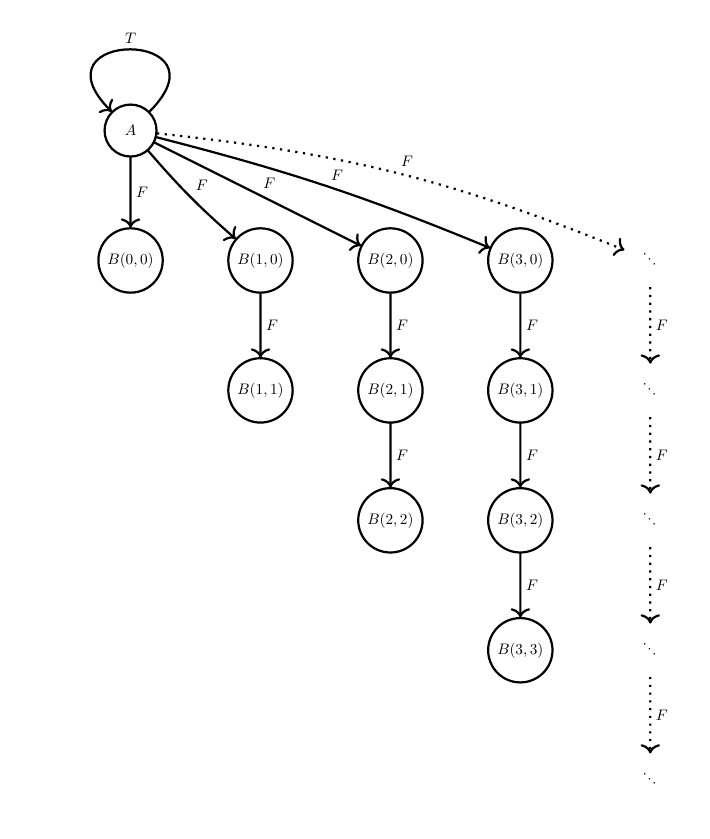
\begin{tikzpicture}[term/.style={circle,draw,minimum size=12mm,inner sep=4pt},auto , scale=0.55, every node/.style={scale=0.55}]
    \node [thick] (A) at (0,0) [term] {$A$};
    \node [thick] (B00) at (0,-3) [term] {$B(0,0)$};
      \node [thick] (B10) at (3,-3) [term] {$B(1,0)$}; \node [thick] (B20) at (6,-3) [term] {$B(2,0)$}; \node [thick] (B30) at (9,-3) [term] {$B(3,0)$}; \node[inner sep=10, rotate=-45] (B40) at (12,-3) {$\cdots$};
    \node [thick] (B11) at (3,-6) [term] {$B(1,1)$}; \node [thick] (B21) at (6,-6) [term] {$B(2,1)$}; \node [thick] (B31) at (9,-6) [term] {$B(3,1)$}; \node[inner sep=10, rotate=-45] (B41) at (12,-6) {$\cdots$};
    \node [thick] (B22) at (6,-9) [term] {$B(2,2)$}; \node [thick] (B32) at (9,-9) [term] {$B(3,2)$};
\node[inner sep=10, rotate=-45] (B42) at (12,-9) {$\cdots$};
    \node [thick] (B33) at (9,-12) [term] {$B(3,3)$};
    \node[inner sep=10, rotate=-45] (B43) at (12,-12) {$\cdots$};
    \node[inner sep=10, rotate=-45] (B44) at (12,-15) {$\cdots$};
%    
    \draw [->,thick,loop] (A) to node[above] {$T$} (A);
    \draw [->,thick] (A) to node {$F$} (B00);
    \draw [->,thick, bend right=4] (A) to node {$F$} (B10);
    \draw [->,thick] (A) to node {$F$} (B20);
    \draw [->,thick, bend left=4] (A) to node {$F$} (B30);
    \draw [->,thick, dotted, bend left=8] (A) to node {$F$} (B40);
%    
    \draw [->,thick] (B10) to node {$F$} (B11);
%
    \draw [->,thick] (B20) to node {$F$} (B21); \draw [->,thick] (B21) to node {$F$} (B22);
%   
    \draw [->,thick] (B30) to node {$F$} (B31); \draw [->,thick] (B31) to node {$F$} (B32); \draw [->,thick] (B32) to node {$F$} (B33);
%
    \draw [->,thick, dotted] (B40) to node {$F$} (B41); \draw [->,thick, dotted] (B41) to node {$F$} (B42); \draw [->,thick, dotted] (B42) to node {$F$} (B43); \draw [->,thick, dotted] (B43) to node {$F$} (B44);
  \end{tikzpicture}
\end{center}

\newcommand{\StrB}{\operatorname{Stream}(B)}
\newcommand{\NodeG}{\operatorname{Node}}

The graph $G$ is an element of a \emph{type} of graphs with nodes $A$ or $B(n,m)$ (with $m\leq n$) and with
edges labelled with a boolean $T$ or $F$. We assume that this type of graphs is available in Iris, just like we assumed that
the type of finite mathematical sequences is, see Section~\ref{sec:basic-separation-logic}. We also assume that
the type of nodes is available and denote it by $\NodeG$.
Moreover, we assume that we have an Iris type of mathematial streams (finite or infinite sequences) available; we write
$\operatorname{Stream}(B)$ for the type of streams of booleans $B=\{T,F\}$, and we write $[]$ for the empty stream,
and $l::ls$ for the stream with head $l$ and tail $ls$.

We will now consider different ways of defining reachability in the graph $G$.
Specifically, we will define predicates that express that, starting from some specific node,
a stream of booleans is reachable in $G$.
(For example, looking at the picture of $G$ above, since there is a loop from node $A$ to $A$
labelled $T$, it is intuitively clear that the constant infinite stream of $T$'s is reachable from $A$.)
Thus we will be interested in predicates on the type $\tau=\NodeG\times \StrB$.

Consider now the following function $F: (\NodeG\times \StrB\to\Prop) \to (\NodeG\times \StrB\to\Prop)$:
\begin{align*}
  F \psi = \lambda (x, ls).\,
    ls = [] \lor
    \exists y, l, ls'.\, ls = l::ls' \land \operatorname{Edge}(G,x,y,l) \land \psi y ls'
\end{align*}
where $\operatorname{Edge}(G,x,y,l)$ means that there is an edge from node $x$ to node $y$ in the graph $G$ with label $l$.

\begin{lemma}
  $F$ is monotone.
\end{lemma}

Since $F$ is monotone, the least and greatest fixed points $\lfp F$ and $\gfp F$ of $F$ exist,
as does the guarded recursive predicate $\grd F$. Each of these define a notion of reachability.


\begin{lemma}
  \label{lem:lfp-gfp-grd}
  \begin{align*}
    \forall x:\tau.\,
    \lfp F x \proves \gfp F x \proves \grd F x.
  \end{align*}
\end{lemma}

The following lemmas express that the inductive notion of reachability
only contains finite paths. 

\begin{lemma}
  \label{lem:lfp-finite}
  Let $ls$ be a \emph{finite} sequence of constant $T$'s or constant $F$'s.
  Then $\lfp F (A,ls)$ holds.
\end{lemma}

\begin{lemma}
  \label{lem:lfp-infinite}
  Let $ls$ be an \emph{infinite} sequence of constant $T$'s or constant $F$'s and let $n$ be any node.
  Then $\lfp F (n,ls)$ does not hold, (i.e., $\lfp F (n,ls) \proves \FALSE$).
\end{lemma}

The following lemmas express that the coinductive notion of reachability
not only includes finite paths, but also infinite paths.


\begin{lemma}
  Let $ls$ be the \emph{infinite} sequence of constant $T$'s.
  Then $\gfp F (A,ls)$ holds.
\end{lemma}

\begin{lemma}
  Let $ls$ be the \emph{infinite} sequence of constant $F$'s and let $n$ be any $B$ node.
  Then $\gfp F (n,ls)$ does not hold (i.e., $\gfp F (n,ls) \proves \FALSE$).
\end{lemma}

\begin{lemma}
  Let $ls$ be the \emph{infinite} sequence of constant $F$'s and let $n$ be any node.
  Then $\gfp F (n,ls)$ does not hold (i.e., $\gfp F (n,ls) \proves \FALSE$).
\end{lemma}

Intuitively, the following lemma captures that guarded-recursive predicates are ``closed under limits'':
by Lemmas \ref{lem:lfp-gfp-grd} and \ref{lem:lfp-finite} every finite path of constant $F$'s is in the guarded-recursive notion of reachability;
this is used to prove the following lemma, which says that also the limit, the \emph{infinite} sequence of constant $F$'s, is in the guarded-recursive notion of reachability.

\begin{lemma}
  Let $ls$ be the \emph{infinite} sequence of constant $F$'s.
  Then $\grd F (A,ls)$ holds.
\end{lemma}

We finally remark that guarded-recursive predicates are in fact unique (we did not include a proof rule expressing that in Section \ref{sec:recursively-defined-pred}) and that is exactly because their behaviour at limit points is determined by what happens at finite approximants.


%%% Local Variables:
%%% mode: latex
%%% TeX-master: "../main.tex"
%%% End:


\input{sections/later-steps.tex}

\input{sections/logical-relations.tex}

\bibliographystyle{plain}
\bibliography{main}

\appendix

\input{sections/overview.tex}

\end{document}

%%% Local Variables:
%%% mode: latex
%%% TeX-master: t
%%% End:
